\chapter{圆}

\section{圆的有关性质}
\subsection{点和圆的位置关系}\label{subsec:czjh2-7-1}

在日常生活中,我们到处都会见到圆形的物体。如各种车轮、茶杯的杯口等都是圆形的。
人们为什么把它们做成圆形的呢?这是因为圆形具有许多有用的性质。
在本章中,我们将详细研究圆的性质及其应用。

如图 \ref{fig:czjh2-7-1}, 线段 $OA$ 绕它固定的一个端点 $O$ 旋转一周,另一个端点 $A$ 所经过的封闭曲线叫做\zhongdian{圆}。
固定的点 $O$ 叫做\zhongdian{圆心}; 线段 $OA$ 叫做\zhongdian{半径}。

\begin{figure}[htbp]
    \centering
    \begin{minipage}[b]{4cm}
        \centering
        \begin{tikzpicture}
    \tkzDefPoints{0/0/O, 1.5/0/A}

    \tkzDrawCircle[thick](O,A)
    \tkzDrawSegment(O,A)
    \tkzDrawPoint(O)
    \tkzLabelSegment[above](O,A){$r$}
    \tkzLabelPoints[left](O)
    \tkzLabelPoints[right](A)
\end{tikzpicture}


        \caption{}\label{fig:czjh2-7-1}
    \end{minipage}
    \qquad
    \begin{minipage}[b]{5cm}
        \centering
        \begin{tikzpicture}
    \tkzDefPoints{0/0/O, 2/0/Q, -0.5/1.0/P}
    \tkzDefPoint(20:1.5){A}

    \tkzDrawCircle[thick](O,A)
    \tkzDrawSegments(O,A  O,P  O,Q)
    \tkzDrawPoints(O,P,Q)
    \tkzLabelSegment[above](O,A){$r$}
    \tkzLabelPoints[left](O,P)
    \tkzLabelPoints[right](Q)
\end{tikzpicture}


        \caption{}\label{fig:czjh2-7-2}
    \end{minipage}
    \qquad
    \begin{minipage}[b]{4.5cm}
        \centering
        \begin{tikzpicture}
    \tkzDefPoints{0/0/O, -1.5/0/A, 1.5/0/B}
    \tkzDefPoint(200:1.5){C}
    \tkzDefPoint(290:1.5){D}

    \tkzDrawCircle[thick](O,A)
    \tkzDrawSegments(A,B  C,D)
    \tkzDrawPoint(O)
    \tkzLabelPoints[left](A,C)
    \tkzLabelPoints[right](B)
    \tkzLabelPoints[below right](D)
    \tkzLabelPoints[below](O)
\end{tikzpicture}


        \caption{}\label{fig:czjh2-7-3}
    \end{minipage}
\end{figure}

从上面的定义可以知道:

(1)圆上各点到定点(圆心 $O$ )的距离都等于定长(半径的长 $r$);

(2)到定点的距离等于定长的点都在圆上。

也就是说,圆是那些到定点的距离等于定长的所有的点组成的图形。

\zhongdian{圆可以看作是到定点的距离等于定长的点的集合。}
定点就是圆心,定长就是半径的长,通常也称为半径。

从画圆的过程中,还可以知道:

圆内各点(如图 \ref{fig:czjh2-7-2} 中的点 $P$)到圆心的距离都小于半径;到圆心的距离小于半径的点都在圆内。
也就是说,\zhongdian{圆的内部可以看作是到圆心的距离小于半径的点的集合。}
圆外各点(如图 \ref{fig:czjh2-7-2} 中的点 $Q$)到圆心的距离都大于半径;到圆心的距离大于半径的点都在圆外。
也就是说,\zhongdian{圆的外部可以看作是到圆心的距离大于半径的点的集合。}

% \begin{figure}[htbp]
%     \centering
%     \begin{minipage}[b]{7cm}
%         \centering
%         \begin{tikzpicture}
    \tkzDefPoints{0/0/O, -1.5/0/A, 1.5/0/B}
    \tkzDefPoint(200:1.5){C}
    \tkzDefPoint(290:1.5){D}

    \tkzDrawCircle[thick](O,A)
    \tkzDrawSegments(A,B  C,D)
    \tkzDrawPoint(O)
    \tkzLabelPoints[left](A,C)
    \tkzLabelPoints[right](B)
    \tkzLabelPoints[below right](D)
    \tkzLabelPoints[below](O)
\end{tikzpicture}


%         \caption{}\label{fig:czjh2-7-3}
%     \end{minipage}
%     \qquad
%     \begin{minipage}[b]{7cm}
%         \centering
%         \begin{tikzpicture}
    \tkzDefPoints{0/0/O}
    \tkzDefPoint(150:1.5){A}
    \tkzDefPoint(95:1.5){B}
    \tkzDefPoint(330:1.5){C}

    \tkzDrawCircle[thick](O,A)
    \tkzDrawSegments[dashed](O,A  O,B  O,C)
    \tkzDrawPoint(O)
    \tkzLabelPoints[left](A)
    \tkzLabelPoints[above](B)
    \tkzLabelPoints[right](C)
    \tkzLabelPoints[below left](O)
\end{tikzpicture}


%         \caption{}\label{fig:czjh2-7-4}
%     \end{minipage}
% \end{figure}


以点 $O$ 为圆心的圆,记作 “$\yuan \, O$”,读作 “圆 $O$”。

连结圆上任意两点的线段(如图 \ref{fig:czjh2-7-3} 中的 $CD$)叫做\zhongdian{弦},
经过圆心的弦(如图 \ref{fig:czjh2-7-3} 中的 $AB$)叫做\zhongdian{直径}。
直径等于半径的 2 倍。


圆上任意两点间的部分叫做\zhongdian{圆弧},简称\zhongdian{弧}。
弧用符号“$\yuanhu{\hspace{1em}}$” 表示。
以 $A$、$B$ 为端点的弧记作 $\yuanhu{AB}$,读作“圆弧 $AB$”,或 “弧 $AB$”。
圆的任定一条直径的两个端点分圆成两条弧,每一条弧都叫做\zhongdian{半圆}。
大于半圆的弧(用三个字母表示,如图 \ref{fig:czjh2-7-4} 中的 $\yuanhu{BAC}$)叫做\zhongdian{优弧};
小于半圆的弧(如图 \ref{fig:czjh2-7-4} 中的 $\yuanhu{BC}$)叫做\zhongdian{劣弧}。

圆心相同、半径不相等的两个圆叫做\zhongdian{同心圆}。
图 \ref{fig:czjh2-7-5} 中的两个圆是以点 $O$ 为圆心的同心圆。

\begin{figure}[htbp]
    \centering
    \begin{minipage}[b]{4cm}
        \centering
        \begin{tikzpicture}
    \tkzDefPoints{0/0/O}
    \tkzDefPoint(150:1.5){A}
    \tkzDefPoint(95:1.5){B}
    \tkzDefPoint(330:1.5){C}

    \tkzDrawCircle[thick](O,A)
    \tkzDrawSegments[dashed](O,A  O,B  O,C)
    \tkzDrawPoint(O)
    \tkzLabelPoints[left](A)
    \tkzLabelPoints[above](B)
    \tkzLabelPoints[right](C)
    \tkzLabelPoints[below left](O)
\end{tikzpicture}


        \caption{}\label{fig:czjh2-7-4}
    \end{minipage}
    \qquad
    \begin{minipage}[b]{4cm}
        \centering
        \begin{tikzpicture}
    \tkzDefPoints{0/0/O}
    \tkzDefPoint(30:1.5){A}
    \tkzDefPoint(160:1.0){B}

    \tkzDrawCircle[thick](O,A)
    \tkzDrawCircle[thick](O,B)
    \tkzDrawSegments(O,A  O,B)
    \tkzDrawPoint(O)
    \tkzLabelSegment[below,yshift=-.3em](O,A){$r_1$}
    \tkzLabelSegment[below](O,B){$r_2$}
    \tkzLabelPoints[below](O)
\end{tikzpicture}


        \caption{}\label{fig:czjh2-7-5}
    \end{minipage}
    \qquad
    \begin{minipage}[b]{5cm}
        \centering
        \begin{tikzpicture}
    \def\drawingcode{
        \tkzDefPoints{0/0/O}
        \tkzDefPoint(35:1.0){A}
        \tkzDrawCircle[thick](O,A)
        \tkzDrawSegment(O,A)
        \tkzDrawPoint(O)
        \tkzLabelSegment[above](O,A){$r$}
    }

    \begin{scope}
        \drawingcode
        \tkzLabelPoint[below](O){$O_1$}
    \end{scope}

    \begin{scope}[xshift=2.5cm]
        \drawingcode
        \tkzLabelPoint[below](O){$O_2$}
    \end{scope}
\end{tikzpicture}


        \caption{}\label{fig:czjh2-7-6}
    \end{minipage}
\end{figure}


能够重合的两个圆叫做\zhongdian{等圆},半径相等的两个圆是等圆。
如图 \ref{fig:czjh2-7-6} 中, $\yuan \, O_1$ 和 $\yuan \, O_2$ 的半径都等于 $r$,所以它们是两个等圆。
反过来,\zhongdian{同圆或等圆的半径相等。}

在同圆或等圆中,能够互相重合的弧叫做\zhongdian{等弧}。


\begin{lianxi}

\xiaoti{设 $AB=3$ 厘米,画图说明具有下列性质的点的集合是怎样的图形:}
\begin{xiaoxiaotis}

    \xxt{和点 $A$ 的距离等于 2 厘米的点的集合;}

    \xxt{和点 $B$ 的距离等于 2 厘米的点的集合;}

    \xxt{和点 $A$、$B$ 的距离都等于 2 厘米的点的集合;}

    \xxt{和点 $A$、$B$ 的距离都小于 2 厘米的点的集合。}

\end{xiaoxiaotis}


\xiaoti{下列各题中的两句话都对吗?如果不对,为什么?}
\begin{xiaoxiaotis}

    \xxt{“直径是弦”、“弦是直径”;}

    \xxt{“半圆是弧”、“弧是半圆”。}

\end{xiaoxiaotis}


\xiaoti{适合下列条件的圆,各画三个:}
\begin{xiaoxiaotis}

    \xxt{以已知点 $O$ 为圆心的圆;}

    \xxt{半径等于 2.5 厘米的圆;}

    \xxt{经过已知点 $A$ 的圈;}

    \xxt{经过已知点 $A$ 和 $B$ 的圆。}

\end{xiaoxiaotis}

\end{lianxi}


\subsection{经过三点的圆}\label{subsec:czjh2-7-2}

我们知道,经过一个点 $A$ 作圆很容易,只要以点 $A$ 以外的任意一点为圆心,
以这一点与点 $A$ 的距离为半径就可以作出。这样的圆有无数多个(图 \ref{fig:czjh2-7-7})。
如果要作通过两个点 $A$、$B$ 的圆,那就要找这样一个点作圆心,
使它与点 $A$、$B$ 的距离都相等,这样的点在线段 $AB$ 的垂直平分线上。
因此,以线段 $AB$ 的垂直平分线上任意一点为圆心,以这一点与点 $A$ 或点 $B$ 的距离为半径就可以作出。
这样的圆也有无数多个(图 \ref{fig:czjh2-7-8})。


\begin{figure}[htbp]
    \centering
    \begin{minipage}[b]{4cm}
        \centering
        \begin{tikzpicture}
    \tkzDefPoints{0/0/A, -1/0/O_1, 0.3/-0.5/O_2, 0.8/0.8/O_3}

    \tkzDrawCircle[thick](O_1,A)
    \tkzDrawCircle[thick](O_2,A)
    \tkzDrawCircle[thick](O_3,A)
    \tkzDrawPoints(O_1, O_2, O_3, A)
    \tkzLabelPoints[above right](A)
    \tkzLabelPoints[below](O_1, O_2)
    \tkzLabelPoints[right](O_3)
\end{tikzpicture}


        \caption{}\label{fig:czjh2-7-7}
    \end{minipage}
    \qquad
    \begin{minipage}[b]{6cm}
        \centering
        \begin{tikzpicture}
    \tkzDefPoints{0/0.5/A, 0/-0.5/B, -1/0/O_1, 0.5/0/O_2, 1.3/0/O_3}

    \tkzDrawLine[add=.7 and .8](O_1, O_3)
    \tkzDrawCircle[thick](O_1,A)
    \tkzDrawCircle[thick](O_2,A)
    \tkzDrawCircle[thick](O_3,A)
    \tkzDrawPoints(O_1, O_2, O_3, A, B)
    \tkzLabelPoints[above=.5em](A)
    \tkzLabelPoints[below=.5em](B)
    \tkzLabelPoints[below](O_1, O_2, O_3)
\end{tikzpicture}


        \caption{}\label{fig:czjh2-7-8}
    \end{minipage}
    \qquad
    \begin{minipage}[b]{4.5cm}
        \centering
        \begin{tikzpicture}
    \tkzDefPoints{0/0/B, 3/0/C, 2/2/A}
    \tkzLabelPoints[above](A)
    \tkzLabelPoints[left](B)
    \tkzLabelPoints[right](C)

    % 1
    \tkzDefLine[mediator, K=.5](A,B)  \tkzGetPoints{E}{D}
    \tkzCompasss(A,D  B,D  A,E  B,E)
    \tkzDrawSegments(A,B  D,E)
    \tkzLabelPoints[above right](D,E)

    % 2
    \tkzDefLine[mediator, K=.5](B,C)  \tkzGetPoints{F}{G}
    \tkzInterLL(D,E)(F,G)  \tkzGetPoint{O}
    \tkzCompasss(B,F  C,F  B,G  C,G)
    \tkzDrawSegments(B,C  F,G)
    \tkzDrawPoint(O)
    \tkzLabelPoints[right](F)
    \tkzLabelPoints[below](G)
    \tkzLabelPoints[below left](O)

    % 3
    \tkzDrawCircle[thick](O,B)

    % ex
    \tkzDrawSegment(A,C)
\end{tikzpicture}


        \caption{}\label{fig:czjh2-7-9}
    \end{minipage}
\end{figure}

现在来讨论,经过三个已知点的圆。

\zhongdian{作圆,使它经过不在同一直线上的三个已知点。}

已知:不在同一直线上的三点 $A$、$B$、$C$(图 \ref{fig:czjh2-7-9})。

求作: $\yuan \, O$,使它经过点 $A$、$B$、$C$。

分析:要作一个圆经过三个已知点 $A$、$B$、$C$,就要确定一个点作圆心,使它到这三点的距离相等。
以前我们学过,三角形三边的垂直平分线相交于一点,这个点到三角形三个顶点的距离相等。
因此可以把 $\triangle ABC$ 三边的垂直平分线的交点作为圆心。

\zuofa 1. 连结 $AB$,作线段 $AB$ 的垂直平分线 $DE$。

2. 连结 $BC$,作线段 $BC$ 的垂直平分线 $FG$,交 $DE$ 于点 $O$。

3. 以 $O$ 为圆心, $OB$ 为半径作圆。

$\yuan\,O$ 就是所求作的圆。

\zhengming 因为 $\yuan\,O$ 的半径等于 $OB$,所以点 $B$ 在 $\yuan\,O$ 上, 就是 $\yuan\,O$ 经过点 $B$。

因为 $O$ 在 $AB$ 的垂直平分线上,所以 $OA = OB$,因此 $\yuan\,O$ 经过点 $A$。
同样可证 $\yuan\,O$ 经过点 $C$。

我们知道,过 $A$、$B$ 两点的圆和过 $B$、$C$两点的圆, 它们的圆心分别在 $AB$ 和 $BC$ 的垂直平分线上。
从上面的作法又可以知道:当已知点 $A$、$B$、$C$ 不在同一直线上时,
$\triangle ABC$ 三边的垂直平分线有一个且只有一个交点,
所以经过点 $A$、$B$、$C$ 可以作一个且只可作一个圆,这就得到:

\begin{dingli}[定理]
    不在同一直线上的三个点确定一个圆。
\end{dingli}

当点 $A$、$B$、$C$ 在同一直线上时,不能作一个圆经过这三点。(为什么?)

由定理可知,经过三角形三个顶点可以作一个圆。
经过三角形各顶点的圆叫做\zhongdian{三角形的外接圆},
外接圆的圆心叫做\zhongdian{三角形的外心},
这个三角形叫做这个\zhongdian{圆的内接三角形}。

一般地,如果一个圆经过多边形的各顶点,这个圆叫做\zhongdian{多边形的外接圆},
这个多边形叫做这个\zhongdian{圆的内接多边形}。

图 \ref{fig:czjh2-7-10} 中,四边形 $ABCD$ 是 $\yuan\,O$ 的内接四边形;
$\yuan\,O$ 是四边形 $ABCD$ 的外接圆。

注意:经过任意四点不一定能作一个圆,所以多于三边的多边形不一定有外接圆。

\begin{figure}[htbp]
    \centering
    \begin{minipage}[b]{4cm}
        \centering
        \begin{tikzpicture}
    \tkzDefPoint(0,0){O}
    \tkzDefPoint(215:1.5){A}
    \tkzDefPoint(325:1.5){B}
    \tkzDefPoint(40:1.5){C}
    \tkzDefPoint(100:1.5){D}

    \tkzDrawPolygon(A,B,C,D)
    \tkzDrawCircle[thick](O,A)
    \tkzDrawPoint(O)
    \tkzLabelPoints[left](A)
    \tkzLabelPoints[right](B,C,O)
    \tkzLabelPoints[above](D)
\end{tikzpicture}


        \caption{}\label{fig:czjh2-7-10}
    \end{minipage}
    \qquad
    \begin{minipage}[b]{5cm}
        \centering
        \begin{tikzpicture}
    \tkzDefPoints{0/0/O}
    \tkzDefPoint(135:1.5){A}
    \tkzDefPoint(45:1.5){B}
    \tkzDefShiftPoint[A](0,-.4){E}
    \tkzDefShiftPoint[B](0,-.4){F}
    \tkzDefLine[mediator](A,B)  \tkzGetPoints{c}{d}
    \tkzInterLL(E,F)(c,d)  \tkzGetPoint{C}
    \tkzDefShiftPoint[C](0,-2.5){D}
    \tkzDefShiftPoint[C](-0.4,0){G}
    \tkzDefShiftPoint[G](0,-2.5){H}

    \tkzDrawCircle[thick](O,A)
    \tkzDrawPolygon[fill=white](A,B,F,C,D,H,G,E) % 为了遮挡住 D 点附近的圆弧
    \tkzDrawPolygon[pattern={mylines[angle=45, distance={4pt}]}](A,B,F,C,D,H,G,E)
    \tkzDrawPoint(O)
    \tkzLabelPoints[left](A)
    \tkzLabelPoints[right](B,D)
    \tkzLabelPoints[below right](C)
\end{tikzpicture}


        \caption*{(第 1 题)}
    \end{minipage}
    \qquad
    \begin{minipage}[b]{4.5cm}
        \centering
        \begin{tikzpicture}
    \tkzDefPoints{0/0/O}
    \tkzDefPoint(60:1.5){A}
    \tkzDefPoint(205:1.5){B}
    \tkzDefPoint(335:1.5){C}

    \tkzDrawPolygon(A,B,C)
    \tkzDrawCircle[thick](O,A)
    \tkzDrawPoint(O)
    \tkzLabelPoints[above](A)
    \tkzLabelPoints[left](B)
    \tkzLabelPoints[right](C,O)
\end{tikzpicture}


        \caption*{(第 4 题)}
    \end{minipage}
\end{figure}

\begin{lianxi}

\xiaoti{(口答)如图, $CD$ 所在直线垂直平分线段 $AB$。为什么使用这样的工具可以找到圆形工件的圆心。}

\xiaoti{作边长分别为 2 厘米、 2.5 厘米、3 厘米的三角形,再作出这个三角形的外接圆,量出这个圆的直径(精确到 0.1 厘米)。}

\xiaoti{作一个直角三角形,作它的外接圆;作一个钝角三角形,作它的外接圆。这两个三角形的外心的位置各是怎样的?}

\xiaoti{按图填空:}
\begin{xiaoxiaotis}

    \xxt{$\triangle ABC$ 是 $\yuan\,O$ 的 \xhx[1cm] 接三角形;}

    \xxt{$\yuan\,O$ 是 $\triangle ABC$ 的 \xhx[1cm] 接圆。}

\end{xiaoxiaotis}

\end{lianxi}




\subsection{垂直于弦的直径}\label{subsec:czjh2-7-3}

把一张圆形的纸片沿着一条直径对折,可以看到,直径两侧的两个半圆能够互相重合。
这说明圆是轴对称图形,而直径所在的直线就是它的对称轴。下面我们来证明这个结论。

\begin{wrapfigure}[9]{r}{4.5cm}
    \centering
    \begin{tikzpicture}
    \tkzDefPoints{0/0/O}
    \tkzDefPoint(90:1.5){C}
    \tkzDefPoint(270:1.5){D}
    \tkzDefPoint(230:1.5){A}
    \tkzDefLine[perpendicular=through A](C,D)  \tkzGetPoint{a}
    \tkzInterLC[common=A](A,a)(O,A)  \tkzGetFirstPoint{A'}
    \tkzInterLL(A,A')(C,D)  \tkzGetPoint{M}

    \tkzDrawCircle[thick](O,A)
    \tkzDrawLine[add=0.2 and 0.2](C,D)
    \tkzDrawSegment(A,A')
    \tkzDrawSegments[dashed](O,A  O,A')
    \tkzMarkRightAngle(A',M,C)
    \tkzDrawPoint(O)
    \tkzLabelPoints[left,xshift=-.3em](A)
    \tkzLabelPoints[right](A', O)
    \tkzLabelPoints[above left](C)
    \tkzLabelPoints[below left](D)
    \tkzLabelPoints[above, xshift=-.6em](M)
\end{tikzpicture}


    \caption{}\label{fig:czjh2-7-11}
\end{wrapfigure}

如图 \ref{fig:czjh2-7-11}, 设 $CD$ 是 $\yuan\,O$ 的任意一条直径,$A$ 为 $\yuan\,O$ 上任意一点。
过点 $A$ 作 $AA' \perp CD$, 交 $\yuan\,O$ 于点 $A'$,垂足为 $M$。连结 $OA$、$OA'$。

在 $\triangle AOA'$ 中,

$\because$ \quad $OA = OA'$, $AA' \perp CD$,

$\therefore$ \quad $AM = MA'$。

即 $CD$ 是 $AA'$ 的垂直平分线,这就是说,对于圆上任意一点 $A$,
在圆上都有关于直线 $CD$ 的对称点 $A'$,因此 $\yuan\,O$ 关于 $CD$ 对称。即

\begin{xingzhi}
    圆是轴对称图形,经过圆心的每一条直线都是对称轴。
\end{xingzhi}

从上面的证明,我们知道,如果 $AA' \perp CD$,那么点 $A$ 和 $A'$ 是对称点,
所以 $AM$ 和 $A'M$、$\yuanhu{AD}$ 和 $\yuanhu{A'D}$ 能够互相重合。于是有下面定理:

\begin{dingli}[垂径定理]
    垂直于弦的直径平分这条弦,并且平分弦所对的弧。
\end{dingli}

由垂径定理,可以推出下面的推论:

\begin{tuilun}[推论1]
    (1)平分弦(不是直径)的直径垂直于弦,并且平分弦所对的弧;
    (2)平分弦所对的一条弧的直径,垂直平分弦;
    (3)弦的垂直平分线经过圆心,并平分弦所对的弧。
\end{tuilun}

\begin{tuilun}[推论2]
    圆的两条平行弦所夹的弧相等。
\end{tuilun}

如图 \ref{fig:czjh2-7-12} 中, $AB \pingxing CD$, 则 $\yuanhu{AC} = \yuanhu{BD}$。

\begin{figure}[htbp]
    \centering
    \begin{minipage}[b]{7cm}
        \centering
        \begin{tikzpicture}
    \tkzDefPoints{0/0/O}
    \tkzDefPoint(90:1.5){M}
    \tkzDefPoint(270:1.5){N}
    \tkzDefPoint(160:1.5){A}
    \tkzDefPoint(20:1.5){B}
    \tkzDefPoint(130:1.5){C}
    \tkzDefPoint(50:1.5){D}

    \tkzDrawCircle[thick](O,A)
    \tkzDrawSegments(M,N  A,B  C,D)
    \tkzDrawPoint(O)
    \tkzLabelPoints[left](A,C)
    \tkzLabelPoints[right](B,D,O)
    \tkzLabelPoints[above](M)
    \tkzLabelPoints[below](N)
\end{tikzpicture}


        \caption{}\label{fig:czjh2-7-12}
    \end{minipage}
    \qquad
    \begin{minipage}[b]{7cm}
        \centering
        \begin{tikzpicture}
    \tkzDefPoints{0/0/O}
    \tkzDefPoint(160:1.5){A}
    \tkzDefPoint(20:1.5){B}
    \tkzDrawArc[thick](O,B)(A)
    \tkzLabelPoints[left](A)
    \tkzLabelPoints[right](B)

    % 1
    \tkzDrawSegment(A,B)

    % 2
    \tkzDefLine[mediator,K=.7](A,B)  \tkzGetPoints{C}{D}
    \tkzInterLC(C,D)(O,A)  \tkzGetFirstPoint{E}
    \tkzCompasss(A,C  B,C  A,D  B,D)
    \tkzDrawLine[add=0.1 and 0.1](C,D)
    \tkzDrawPoint(E)
    \tkzLabelPoints[right](C,D)
    \tkzLabelPoints[above right](E)
\end{tikzpicture}


        \caption{}\label{fig:czjh2-7-13}
    \end{minipage}
\end{figure}

\liti 平分已知 $\yuanhu{AB}$。

已知: $\yuanhu{AB}$(图 \ref{fig:czjh2-7-13})。

求作:$\yuanhu{AB}$ 的中点。

\zuofa 1. 连结 $AB$。

2. 作 $AB$ 的垂直平分线 $CD$,交 $\yuanhu{AB}$ 于点 $E$。

点 $E$ 就是所求 $\yuanhu{AB}$ 的中点。

证明略。


\liti 一千三百多年前,我国隋代建造的赵州石拱桥(图 \ref{fig:czjh2-7-14})的桥拱是圆弧形,
它的跨度(弧所对的弦的长)为 37.4 米,拱高(弧的中点到弦的距离,也叫弓形高)为7.2米,
求桥拱的半径(精确到 0.1 米)。

\begin{figure}[htbp]
    \centering
    \begin{minipage}[b]{10.5cm}
        \centering
        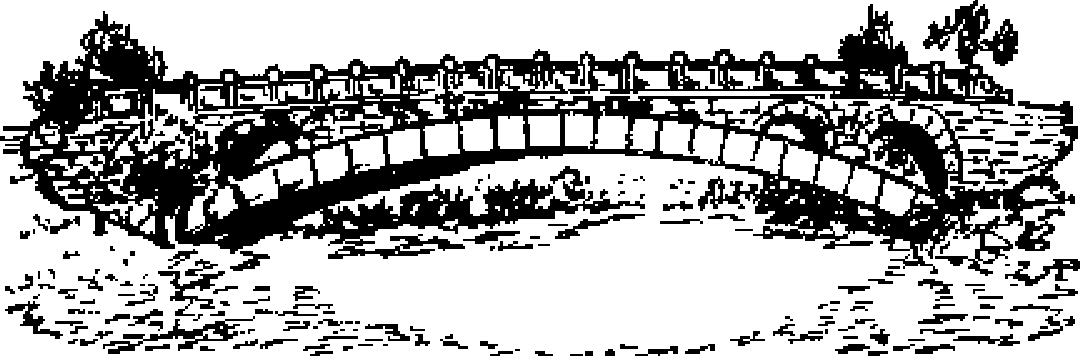
\includegraphics[width=10cm]{../pic/czjh2-ch7-14.png}
        \caption{}\label{fig:czjh2-7-14}
    \end{minipage}
    \qquad
    \begin{minipage}[b]{5cm}
        \centering
        \begin{tikzpicture}[>=Stealth,]
    \pgfmathsetmacro{\factor}{0.1}
    \tkzDefPoints{0/0/O}
    \tkzDefPoint(90:27.9*\factor){C}
    \tkzDefPointOnLine[pos=7.2/37.4](C,O)  \tkzGetPoint{D}
    \tkzDefLine[perpendicular=through D](O,C)  \tkzGetPoint{a}
    \tkzInterLC(D,a)(O,C)  \tkzGetPoints{B}{A}

    \tkzDrawArc[thick](O,B)(A)
    \tkzDrawSegments[dashed](O,C A,B B,O O,A)
    \tkzMarkRightAngle[size=0.2](A,D,O)
    \tkzLabelSegment[below left](O,A){$R$}
    \tkzLabelPoints[below,xshift=-.3em](A)
    \tkzLabelPoints[below right](B)
    \tkzLabelPoints[below right](C)
    \tkzLabelPoints[below right](D)
    \tkzLabelPoints[below](O)

    %
    \tkzDefPointBy[translation=from D to C](A)  \tkzGetPoint{E}
    \tkzDefShiftPoint[A](-0.5,0){Ha}
    \tkzDefPointBy[translation=from A to Ha](E)  \tkzGetPoint{He}
    \tkzDefShiftPoint[Ha](0,-0.3){Has}
    \tkzDefShiftPoint[He](0, 0.3){Hes}
    \tkzDrawLine[add=0 and 0.4](A,Ha)  \tkzDrawSegments(C,E)
    \tkzDrawLine[add=0 and 0.4](E,He)
    \tkzDrawSegment[-latex](Has,Ha)
    \tkzDrawSegment[-latex](Hes,He)
    \tkzLabelSegment[rotate=90,yshift=.5em](Ha,He){\footnotesize $7.2$}

    \tkzDefShiftPoint[A](0, 0.9){Wa}
    \tkzDefShiftPoint[B](0, 0.9){Wb}
    \tkzDrawLines[add=0 and 0.3](A,Wa  B,Wb)
    \tkzDrawSegment[latex-latex](Wa,Wb)
    \tkzLabelSegment[yshift=.5em,fill=white, inner sep=1pt](Wa,Wb){$37.4$}
    % \draw [latex-latex] (Wa) to [xianduan] node [fill=white, inner sep=1pt]{$30$} (Wb);
    % \tkzDrawSegment[dim={$37.4$,10pt,}](Wa,Wb)
\end{tikzpicture}


        \caption{}\label{fig:czjh2-7-15}
    \end{minipage}
\end{figure}

\jie 如图 \ref{fig:czjh2-7-15}, 用 $\yuanhu{AB}$ 表示桥拱, $\yuanhu{AB}$ 的圆心为 $O$、半径为 $R$ 米。
经过圆心 $O$ 作弦 $AB$ 的垂线 $OD$, $D$为垂足, 与 $\yuanhu{AB}$ 相交于点 $C$。
根据垂径定理, $D$ 是 $AB$ 的中点, $C$ 是 $\yuanhu{AB}$ 的中点, $CD$ 就是拱高。由题设
\begin{gather*}
    AB = 37.4 \douhao  CD = 7.2 \douhao \\
    AD = \exdfrac{1}{2} AB = \exdfrac{1}{2} \times 37.4 = 18.7 \douhao \\
    OD = OC - DC = R - 7.2 \juhao
\end{gather*}

在 $Rt \triangle OAD$ 中,由勾股定理,得
$$ OA^2 = AD^2 + OD^2 \douhao $$

即 $R^2 = 18.7^2 + (R - 7.2)^2 \juhao $

解这个方程,得 $R \approx 27.9$(米)。

答: 赵州石拱桥的桥拱半径约为 27.9 米。


\begin{lianxi}

\xiaoti{(口答)}%
\begin{xiaoxiaotis}%
    \xxt[-1em]{平分一条弧的直径有什么性质?}

    \xxt{平分弦和它所对的一条弧的直线有什么性质?}

    \xxt{垂直弦,并平分弦所对的一条弧的直线有什么性质?}

\end{xiaoxiaotis}

\xiaoti{在平径为 50 mm 的 $\yuan\,O$ 中, 有长 50 mm 的弦 $AB$。计算:}
\begin{xiaoxiaotis}

    \xxt{点 $O$ 与 $AB$ 的距离;}

    \xxt{$\angle AOB$ 的度数。}

\end{xiaoxiaotis}

\xiaoti{以点 $O$ 为圆心的两个同心圆中,大圆的弦 $AB$ 和小圆相交于点 $C$ 和 $D$。
    求证: $AC = BD$。
}

\end{lianxi}


\subsection{圆心角、弧、弦、弦心距之间的关系}\label{subsec:czjh2-7-4}

如图 \ref{fig:czjh2-7-16} 甲 ,在 $\yuan\,O$ 上任取一点 $A$,作直径 $AB$,则 $OA = OB$。
就是说,点 $B$ 是点 $A$ 关于点 $O$ 的对称点。
因此,\zhongdian{圆是以圆心为对称中心的中心对称图形。}

\begin{figure}[htbp]
    \centering
    \begin{minipage}[b]{6cm}
        \centering
        \begin{tikzpicture}
    \tkzDefPoints{0/0/O}
    \tkzDefPoint(155:1.5){A}
    \tkzDefPoint(335:1.5){B}

    \tkzDrawCircle[thick](O,A)
    \tkzDrawSegments(O,A  O,B)
    \tkzDrawPoint(O)
    \tkzLabelPoints[above](O)
    \tkzLabelPoints[left](A)
    \tkzLabelPoints[right](B)
\end{tikzpicture}


        \caption*{甲}
    \end{minipage}
    \qquad
    \begin{minipage}[b]{6cm}
        \centering
        \begin{tikzpicture}
    \tkzDefPoints{0/0/O}
    \tkzDefPoint(0:1.5){A}
    \tkzDefPoint(40:1.5){B}

    \tkzDrawCircle[thick](O,A)
    \tkzDrawSegments(O,A  O,B)
    \tkzMarkAngle[size=.6, -latex](A,O,B)
    \tkzLabelAngle[pos=.8](A,O,B){$\alpha$}
    \tkzDrawPoint(O)
    \tkzLabelPoints[left](O)
    \tkzLabelPoints[right](A,B)
\end{tikzpicture}


        \caption*{乙}
    \end{minipage}
    \caption{}\label{fig:czjh2-7-16}
\end{figure}

圆不仅是中心对称图形:绕圆心旋转 $180^\circ$ 后能够与原来的图形重合,并且它还有另外一个重要性质。
如图 \ref{fig:czjh2-7-16} 乙中,让圆绕中心 $O$ 旋转任意一个角度 $\alpha$, 圆上任意一点 $A$ 都能够与圆上一点 $B$ 重合。
因此,圆绕圆心旋转任意一个角度,都能够与原来的图形重合。
利用这个性质,我们还可以推出圆的其他一些性质。

顶点在圆心的角叫做\zhongdian{圆心角}。 从圆心到弦的距离叫做\zhongdian{弦心距}。
现在用上面的性质来研究在同一个圆中,圆心角、圆心角所对的弦、弧、弦心距相互之间的关系。

如图 \ref{fig:czjh2-7-17} $\yuan\,O$ 中,当圆心角 $\angle AOB = \angle A'OB'$ 时,
它们所对的弧 $\yuanhu{AB}$ 和 $\yuanhu{A'B'}$、弦 $AB$ 和 $A'B'$、
弦心距 $OM$ 和 $OM'$ 是否也相等呢?

我们把 $\angle AOB$ 连同 $\yuanhu{AB}$ 绕圆心 $O$ 旋转,使射线 $OA$ 与 $OA'$ 重合。

$\because$ \quad $\angle AOB = \angle A'OB'$,

$\therefore$ \quad  射线 $OB$ 与 $OB'$ 重合。

又$\because$ \quad  $OA = OA'$, $OB = OB'$,

$\therefore$ \quad 点 $A$ 和点 $A'$ 重合,点 $B$ 与点 $B'$ 重合。

这样,$\yuanhu{AB}$ 与 $\yuanhu{A'B'}$ 重合, $AB$ 与 $A'B'$ 重合,
从点 $O$ 到 $AB$ 的垂线段 $OM$ 和点 $O$ 到 $A'B'$ 的垂线段 $OM'$ 也重合。即
$$ \yuanhu{AB} = \yuanhu{A'B'} \douhao  AB = A'B' \douhao  OM = OM' \juhao $$

\begin{figure}[htbp]
    \centering
    \begin{minipage}[b]{4cm}
        \centering
        \begin{tikzpicture}
    \tkzDefPoints{0/0/O}
    \tkzDefPoint(0:1.5){A}
    \tkzDefPoint(50:1.5){B}
    \tkzDefPoint(80:1.5){A'}
    \tkzDefPoint(130:1.5){B'}
    \tkzDefLine[altitude](A,O,B)  \tkzGetPoint{M}
    \tkzDefLine[altitude](A',O,B')  \tkzGetPoint{M'}

    \tkzDrawCircle[thick](O,A)
    \tkzDrawSegments     (O,A   O,B   A,B    O,M)
    \tkzDrawSegments[red](O,A'  O,B'  A',B'  O,M')
    \tkzMarkAngle[size=.6, -latex](A,O,A')
    \tkzDrawPoint(O)
    \tkzLabelPoints[below left](O)
    \tkzLabelPoints[right](A)
    \tkzLabelPoints[above right](B)
    \tkzLabelPoints[above](A')
    \tkzLabelPoints[above](B')
    \tkzLabelPoints[below, xshift=-.4em](M)
    \tkzLabelPoints[below, xshift=-.3em](M')
\end{tikzpicture}


        \caption{}\label{fig:czjh2-7-17}
    \end{minipage}
    \qquad
    \begin{minipage}[b]{6cm}
        \centering
        \begin{tikzpicture}
    \tkzDefPoints{0/0/O}
    \tkzDefPoint(-40:1.5){A}
    \tkzDefPoint(20:1.5){B}
    \tkzDefPoint(50:1.5){C}
    \tkzDefPoint(51:1.5){D}

    \tkzDrawCircle[thick](O,A)
    \tkzDrawSegments(O,A  O,B  O,C  O,D)
    \tkzMarkAngle[size=.6](A,O,B)
    \tkzDrawPoint(O)
    \tkzLabelPoints[left](O)
    \tkzLabelPoints[right](A,B)

    %
    \tkzDefPoint(-20:0.6){e1}  % End point
    \tkzDefPoint(-20:1.8){b1}  % Begin point
    \tkzDrawSegment[-latex](b1,e1)
    \tkzLabelSegment[pos=0, right](b1,e1){$n^\circ$圆心角}

    \tkzDefPoint(5:1.5){e2}
    \tkzDefPoint(5:1.8){b2}
    \tkzDrawSegment[-latex](b2,e2)
    \tkzLabelSegment[pos=0, right](b2,e2){$n^\circ$弧}

    \tkzDefPoint(50.5:1.2){e3}
    \tkzDefPoint(30:1.8){b3}
    \tkzDrawSegment[-latex](b3,e3)
    \tkzLabelSegment[pos=0, right](b3,e3){$1^\circ$圆心角}

    \tkzDefPoint(50.5:1.5){e4}
    \tkzDefPoint(45:1.8){b4}
    \tkzDrawSegment[-latex](b4,e4)
    \tkzLabelSegment[pos=0, right, yshift=.3em](b4,e4){$1^\circ$弧}
\end{tikzpicture}


        \caption{}\label{fig:czjh2-7-18}
    \end{minipage}
    \qquad
    \begin{minipage}[b]{4.5cm}
        \centering
        \begin{tikzpicture}
    \tkzDefPoints{0/0/O}
    \tkzDefPoint(285:1.5){A}
    \tkzDefPoint(105:1.5){B}
    \tkzDefPoint(230:1.5){D}
    \tkzDefPoint(50:1.5){E}
    \tkzDefLine[parallel=through A](D,E)  \tkzGetPoint{c}
    \tkzInterLC[common=A](A,c)(O,A)  \tkzGetFirstPoint{C}

    \tkzDrawCircle[thick](O,A)
    \tkzDrawSegments(A,B  D,E)
    \tkzDrawSegments(A,C  C,E  E,B)
    \tkzDrawPoint(O)
    \tkzLabelPoints[left](O)
    \tkzLabelPoints[below](A,D)
    \tkzLabelPoints[above](B,E)
    \tkzLabelPoints[right](C)
\end{tikzpicture}


        \caption{}\label{fig:czjh2-7-19}
    \end{minipage}
\end{figure}

上面的结论,在两个等圆中也成立。于是有下面的定理:

\begin{dingli}[定理]
    在同圆或等圆中,相等的圆心角所对的弧相等,所对的弦相等,所对的弦的弦心距相等。
\end{dingli}

由上面的定理,可以得到下面推论:

\begin{tuilun}[推论]
    在同圆或等圆中,如果两个圆心角、两条弧、两条弦或两条弦的弦心距中有一组量相等,
    那么它们所对应的其余各组量都分别相等。
\end{tuilun}

我们知道,把顶点在圆心的周角等分成 360 份时,每一份的圆心角是 $1^\circ$ 的角。
因为同圆中相等的圆心角所对的弧相等,所以整个圆也被等分成 360 份。
我们把每一份这样的弧叫做 \zhongdian{$\bm{1^\circ}$ 的弧}。

由上述定义可知, $1^\circ$ 的圆心角对着 $1^\circ$ 的弧, $1^\circ$ 的弧对着 $1^\circ$ 的圆心角。
一般地, $n^\circ$ 的圆心角对着 $n^\circ$ 的弧, $n^\circ$ 的弧对着 $n^\circ$ 的圆心角(图 \ref{fig:czjh2-7-18})。
也就是说,圆心角的度数和它所对的弧的度数相等。


\liti[0] 如图 \ref{fig:czjh2-7-19}, $AB$、$DE$ 是 $\yuan\,O$ 的直径, $AC \pingxing DE$,交 $\yuan\,O$ 于点 $C$。

求证:  $BE = EC$。

\zhengming 在 $\yuan\,O$ 中,

$\left.\begin{aligned}
    \angle AOD = \angle BOE  \tuichu \yuanhu{AD} = \yuanhu{BE} \\
    AC \pingxing DE  \tuichu \yuanhu{AD} = \yuanhu{EC}
\end{aligned}\right\}  \tuichu \yuanhu{BE} = \yuanhu{EC}  \tuichu  BE = EC \juhao$


\begin{lianxi}

\xiaoti{如图,$\yuan\,O$ 的弦 $AB > CD$, $AB$、$CD$ 的弦心距分别为 $OM$ 和 $ON$。
    求证:$OM < ON$。
}

\begin{figure}[htbp]
    \centering
    \begin{minipage}[b]{7cm}
        \centering
        \begin{tikzpicture}
    \tkzDefPoints{0/0/O}
    \tkzDefPoint(315:1.5){A}
    \tkzDefPoint(45:1.5){B}
    \tkzDefPoint(110:1.5){C}
    \tkzDefPoint(160:1.5){D}
    \tkzDefLine[altitude](A,O,B)  \tkzGetPoint{M}
    \tkzDefLine[altitude](C,O,D)  \tkzGetPoint{N}

    \tkzDrawCircle[thick](O,A)
    \tkzDrawSegments[dashed](O,A  O,B  O,C  O,D)
    \tkzDrawSegments(A,B  C,D  O,M  O,N)
    \tkzMarkRightAngle(B,M,O)
    \tkzMarkRightAngle(O,N,C)
    \tkzDrawPoint(O)
    \tkzLabelPoints[below](O)
    \tkzLabelPoints[below](A)
    \tkzLabelPoints[right](B)
    \tkzLabelPoints[above](C)
    \tkzLabelPoints[left](D)
    \tkzLabelPoints[right,xshift=-.3em](M)
    \tkzLabelPoints[below=.2em](N)
\end{tikzpicture}


        \caption*{(第 1 题)}
    \end{minipage}
    \qquad
    \begin{minipage}[b]{7cm}
        \centering
        \begin{tikzpicture}
    \tkzDefPoints{0/0/P,  3/0/O,  4.5/0/M}
    \tkzDefPoint(15:5){E}
    \tkzDefPoint(-15:5){F}
    \tkzInterLC(P,E)(O,M)  \tkzGetPoints{B}{A}
    \tkzInterLC(P,F)(O,M)  \tkzGetPoints{C}{D}

    \tkzDrawSegments(P,E  P,F)
    \tkzDrawLine[add=0 and .8](P,O)
    \tkzDrawCircle(O,M)
    \tkzDrawPoint(O)
    \tkzMarkAngle[size=.6, arc=ll](F,P,O)
    \tkzMarkAngle[size=.8, arc=ll](O,P,E)

    \tkzLabelPoints[left](P)
    \tkzLabelPoints[right](E,F)
    \tkzLabelPoints[above](O)
    \tkzLabelPoints[above,xshift=-.3em](A)
    \tkzLabelPoints[above](B)
    \tkzLabelPoints[below,xshift=-.3em](C)
    \tkzLabelPoints[below](D)
\end{tikzpicture}


        \caption*{(第 2 题)}
    \end{minipage}
\end{figure}

\xiaoti{设 $O$ 是 $\angle EPF$ 的平分线上的一点,以 $O$ 为圆心的圆和角的两边分别相交于 $A$、$B$
    和 $C$、$D$。求证: $AB = CD$。
}

\xiaoti{(口答)在半径不等的 $\yuan\,O$ 和 $\yuan\,O'$ 中, $\yuanhu{AB}$ 和 $\yuanhu{A'B'}$
    所对的圆心角都是 $60^\circ$。
}
\begin{xiaoxiaotis}

    \xxt{$\yuanhu{AB}$ 和 $\yuanhu{A'B'}$ 各是多少度?}

    \xxt{$\yuanhu{AB}$ 和 $\yuanhu{A'B'}$ 相等吗?}

\end{xiaoxiaotis}


\end{lianxi}
\subsection{圆周角}\label{subsec:czjh2-7-5}
\begin{enhancedline}

顶点在圆上并且两边都和圆相交的角,叫做\zhongdian{圆周角}。
图 \ref{fig:czjh2-7-20} 各圆中的 $\angle BAC$ 都是圆周角。

\begin{dingli}[定理]
    一条弧所对的圆周角等于它所对的圆心角的一半。
\end{dingli}

已知: $\yuan\,O$ 中, $\yuanhu{BC}$ 所对的圆周角是 $\angle BAC$,圆心角是 $\angle BOC$ (图 \ref{fig:czjh2-7-20})。

\begin{figure}[htbp]
    \centering
    \begin{minipage}[b]{4cm}
        \centering
        \begin{tikzpicture}
    \tkzDefPoints{0/0/O}
    \tkzDefPoint(55:1.5){A}
    \tkzDefPoint(235:1.5){B}
    \tkzDefPoint(330:1.5){C}

    \tkzDrawCircle[thick](O,A)
    \tkzDrawSegments(O,A  O,B  O,C  A,C)
    \tkzLabelPoints[above left](O)
    \tkzLabelPoints[above right](A)
    \tkzLabelPoints[right](C)
    \tkzLabelPoints[below left](B)
\end{tikzpicture}


        \caption*{甲}
    \end{minipage}
    \qquad
    \begin{minipage}[b]{4cm}
        \centering
        \begin{tikzpicture}
    \tkzDefPoints{0/0/O}
    \tkzDefPoint(55:1.5){A}
    \tkzDefPoint(200:1.5){B}
    \tkzDefPoint(330:1.5){C}
    \tkzDefPoint(235:1.5){D}

    \tkzDrawCircle[thick](O,A)
    \tkzDrawPolygon(A,B,O,C)
    \tkzDrawSegment[dashed](A,D)
    \tkzLabelPoints[right, yshift=.3em](O)
    \tkzLabelPoints[above right](A)
    \tkzLabelPoints[right](C)
    \tkzLabelPoints[left](B)
    \tkzLabelPoints[below left](D)
\end{tikzpicture}


        \caption*{乙}
    \end{minipage}
    \qquad
    \begin{minipage}[b]{4cm}
        \centering
        \begin{tikzpicture}
    \tkzDefPoints{0/0/O}
    \tkzDefPoint(55:1.5){A}
    \tkzDefPoint(255:1.5){B}
    \tkzDefPoint(330:1.5){C}
    \tkzDefPoint(235:1.5){D}

    \tkzDrawCircle[thick](O,A)
    \tkzDrawPolygon(A,B,O,C)
    \tkzDrawSegment[dashed](A,D)
    \tkzLabelPoints[left](O)
    \tkzLabelPoints[above right](A)
    \tkzLabelPoints[right](C)
    \tkzLabelPoints[below](B)
    \tkzLabelPoints[below left](D)
\end{tikzpicture}


        \caption*{丙}
    \end{minipage}
    \caption{}\label{fig:czjh2-7-20}
\end{figure}

求证: $\angle BAC = \exdfrac{1}{2} \angle BOC$。

\zhengming 分三种情况讨论。

(1) 图 \ref{fig:czjh2-7-20} 甲中,圆心 $O$  在 $\angle BAC$ 的一条边上。

$\left.\begin{aligned}
    OA = OC  \tuichu  \angle C = \angle  BAC \\
    \angle BOC = \angle BAC + \angle C
\end{aligned}\right\}  \tuichu \angle BAC = \exdfrac{1}{2} \angle BOC \juhao$

(2) 图 \ref{fig:czjh2-7-20} 乙中,圆心 $O$  在 $\angle BAC$ 的内部。

作直径 $AD$。 利用(1)的结果,有

$\left.\begin{aligned}
    \angle BAD = \exdfrac{1}{2} \angle BOD \\
    \angle DAC = \exdfrac{1}{2} \angle DOC
\end{aligned}\right\}  \tuichu  \angle BAD + \angle DAC = \exdfrac{1}{2} (\angle BOD + \angle DOC)  \tuichu  \angle BAC = \exdfrac{1}{2} \angle BOC \juhao$

(3) 图 \ref{fig:czjh2-7-20} 丙中,圆心 $O$  在 $\angle BAC$ 的外部。

作直径 $AD$。 利用(1)的结果,有

$\left.\begin{aligned}
    \angle DAB = \exdfrac{1}{2} \angle DOB \\
    \angle DAC = \exdfrac{1}{2} \angle DOC
\end{aligned}\right\}  \tuichu  \angle DAC - \angle DAB = \exdfrac{1}{2} (\angle DOC - \angle DOB)  \tuichu  \angle BAC = \exdfrac{1}{2} \angle BOC \juhao$

由定理可推得下面一些推论:

\begin{tuilun}[推论1]
    同弧或等弧所对的圆周角相等;
    同圆或等圆中,相等的圆周角所对的弧也相等。
\end{tuilun}(图 \ref{fig:czjh2-7-21})

\begin{figure}[htbp]
    \centering
    \begin{minipage}[b]{4.5cm}
        \centering
        \begin{tikzpicture}
    \tkzDefPoints{0/0/O}
    \tkzDefPoint(225:1.5){A}
    \tkzDefPoint(315:1.5){B}
    \tkzDefPoint(150:1.5){C_1}
    \tkzDefPoint(95:1.5){C_2}
    \tkzDefPoint(10:1.5){C_3}

    \tkzDrawCircle[thick](O,A)
    \tkzDrawSegments(A,B)
    \tkzDrawSegments(A,C_1  A,C_2  A,C_3)
    \tkzDrawSegments(B,C_1  B,C_2  B,C_3)
    \tkzDrawPoint(O)
    \tkzLabelPoints[above](O)
    \tkzLabelPoints[left](A)
    \tkzLabelPoints[right](B)
    \tkzLabelPoints[left](C_1)
    \tkzLabelPoints[above](C_2)
    \tkzLabelPoints[right](C_3)
\end{tikzpicture}


        \caption{}\label{fig:czjh2-7-21}
    \end{minipage}
    \qquad
    \begin{minipage}[b]{4.5cm}
        \centering
        \begin{tikzpicture}
    \tkzDefPoints{0/0/O}
    \tkzDefPoint(180:1.5){A}
    \tkzDefPoint(0:1.5){B}
    \tkzDefPoint(130:1.5){C_1}
    \tkzDefPoint(90:1.5){C_2}
    \tkzDefPoint(40:1.5){C_3}

    \tkzDrawCircle[thick](O,A)
    \tkzDrawSegments(A,B)
    \tkzDrawSegments(A,C_1  A,C_2  A,C_3)
    \tkzDrawSegments(B,C_1  B,C_2  B,C_3)
    \tkzDrawPoint(O)
    \tkzMarkRightAngle(A,C_1,B)
    \tkzMarkRightAngle(A,C_2,B)
    \tkzMarkRightAngle(A,C_3,B)
    \tkzLabelPoints[below](O)
    \tkzLabelPoints[left](A)
    \tkzLabelPoints[right](B)
    \tkzLabelPoints[left,yshift=.3em](C_1)
    \tkzLabelPoints[above](C_2)
    \tkzLabelPoints[right](C_3)
\end{tikzpicture}


        \caption{}\label{fig:czjh2-7-22}
    \end{minipage}
    \qquad
    \begin{minipage}[b]{4.5cm}
        \centering
        \begin{tikzpicture}
    \tkzDefPoints{0/0/O}
    \tkzDefPoint(180:1.5){A}
    \tkzDefPoint(0:1.5){B}
    \tkzDefPoint(70:1.5){C}

    \tkzDrawCircle[thick](O,A)
    \tkzDrawSegments(A,B)
    \tkzDrawSegments(A,C  B,C  O,C)
    \tkzDrawPoint(O)
    \tkzMarkRightAngle(A,C,B)
    \tkzLabelPoints[below](O)
    \tkzLabelPoints[left](A)
    \tkzLabelPoints[right](B)
    \tkzLabelPoints[above](C)
\end{tikzpicture}


        \caption{}\label{fig:czjh2-7-23}
    \end{minipage}
\end{figure}

\begin{tuilun}[推论2]
    半圆(或直径)所对的圆周角是直角;
    $90^\circ$ 的圆周角所对的弦是直径。
\end{tuilun}(图 \ref{fig:czjh2-7-22})

如图 \ref{fig:czjh2-7-23},在 $\triangle ABC$ 中,如果中线 $CO = \exdfrac{1}{2} AB$,
以 $AB$ 为直径作 $\yuan\,O$, 则点 $C$ 在 $\yuan\,O$ 上。
由推论 2 可知, $\angle ACB = Rt \angle$。 由此得到:

\begin{tuilun}[推论3]
    如果三角形一边上的中线等于这边的一半,那么这个三角形是直角三角形。
\end{tuilun}

由弦及其所对的弧组成的图形叫做\zhongdian{弓形}。
如图 \ref{fig:czjh2-7-21},弦 $AB$ 与 $\yuanhu{AC_2B}$ 组成弓形 $AC_2B$。
图中的 $\angle AC_2B$ 也可以叫做 $\yuanhu{AC_2B}$ 所含的圆周角,
或 $\yuanhu{AC_2B}$ 所含的\zhongdian{弓形角}。


\liti 如图 \ref{fig:czjh2-7-24}, $AD$ 是 $\triangle ABC$ 的高, AE是 $\triangle ABC$  的外接圆直径。

求证: $AB \cdot AC = AE \cdot AD$。

\zhengming 连结 $BE$。

$\because$ \quad $\angle ADC = \angle ABE = Rt \angle$, $\angle C = \angle E$,

$\therefore$ \quad $\triangle ADC \xiangsi \triangle ABE$。

$\therefore$ \quad $\dfrac{AC}{AE} = \dfrac{AD}{AB}$。

$\therefore$ \quad $AB \cdot AC = AE \cdot AD$。


\begin{figure}[htbp]
    \centering
    \begin{minipage}[b]{4.5cm}
        \centering
        \begin{tikzpicture}
    \tkzDefPoints{0/0/O}
    \tkzDefPoint(70:1.5){A}
    \tkzDefPoint(200:1.5){B}
    \tkzDefPoint(340:1.5){C}
    \tkzDefLine[altitude](C,A,B)  \tkzGetPoint{D}
    \tkzInterLC[common=A](A,O)(O,A)  \tkzGetFirstPoint{E}

    \tkzDrawPolygon(A,B,C)
    \tkzDrawCircle[thick](O,A)
    \tkzDrawSegments(A,D  A,E)
    \tkzDrawSegments[dashed](B,E)
    \tkzDrawPoint(O)
    \tkzMarkRightAngle(A,D,C)
    \tkzLabelPoints[right](O)
    \tkzLabelPoints[above](A)
    \tkzLabelPoints[left](B)
    \tkzLabelPoints[right](C)
    \tkzLabelPoints[below](D)
    \tkzLabelPoints[below](E)
\end{tikzpicture}


        \caption{}\label{fig:czjh2-7-24}
    \end{minipage}
    \qquad
    \begin{minipage}[b]{4.5cm}
        \centering
        \begin{tikzpicture}
    \tkzDefPoints{0/0/O}
    \tkzDefPoint(210:1.5){A}
    \tkzDefPoint(330:1.5){B}
    \tkzDefPoint(80:1.5){M}
    \tkzDefPoint(160:1.0){P}
    \tkzDefPoint(35:2.0){Q}
    \tkzInterLC[common=A](A,P)(O,A)  \tkzGetFirstPoint{P'}
    \tkzInterLC[common=A](A,Q)(O,A)  \tkzGetFirstPoint{Q'}

    \tkzDrawArc[thick](O,B)(A)
    \tkzDrawSegments(A,B  A,P  A,Q  B,P  B,Q)
    \tkzDrawSegments[dashed](P,P'  B,P'  B,Q')
    \tkzLabelPoints[left](A)
    \tkzLabelPoints[right](B, Q)
    \tkzLabelPoints[above](M, P')
    \tkzLabelPoints[above, xshift=.2em](Q')
    \tkzLabelPoints[left](P)
\end{tikzpicture}


        \caption{}\label{fig:czjh2-7-25}
    \end{minipage}
    \qquad
    \begin{minipage}[b]{6cm}
        \centering
        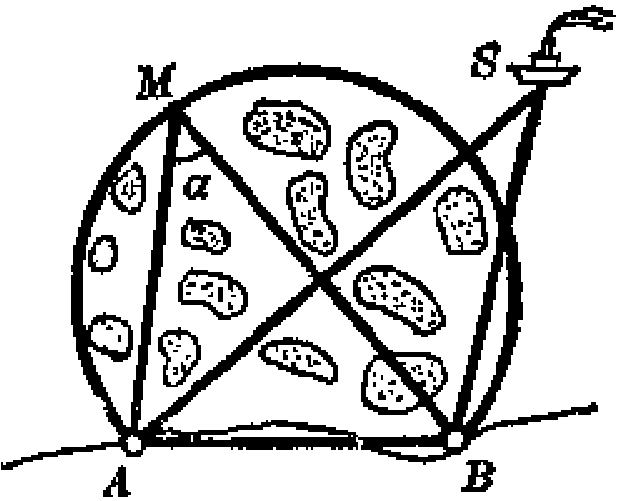
\includegraphics[width=5.5cm]{../pic/czjh2-ch7-26.png}
        \caption{}\label{fig:czjh2-7-26}
    \end{minipage}
\end{figure}


\liti 已知: 如图 \ref{fig:czjh2-7-25}, $P$ 是弓形 $AMB$ 内任意一点, $Q$ 是弓形外的任意一点,
并且和点 $P$ 在直线 $AB$ 同侧。弓形角等于 $\alpha$。

求证:(1) $\angle APB > \alpha$; (2)$\angle AQB < \alpha$。

\zhengming (1) 延长 $AP$ 交 $\yuanhu{AMB}$ 于点 $P'$。连结 $BP'$。

$\because$ \quad 点 $P'$ 在弓形弧上,

$\therefore$ \quad $\angle AP'B = \alpha$。

又 $\because$ \quad $\angle APB$ 是 $\triangle PP'B$ 的外角,

$\therefore$ \quad $\angle APB > \angle AP'B = \alpha$。

(2)设 $AQ$ 与 $\yuanhu{AMB}$ 交于点 $Q'$,连结 $BQ'$。

$\because$ \quad 点 $Q'$ 在弓形弧上,

$\therefore$ \quad $\angle AQ'B = \alpha$。

又 $\because$ \quad $\angle AQ'B$ 是 $\triangle BQ'Q$ 的外角。

$\therefore$ \quad $\angle AQB < \angle AQ'B = \alpha$。


例2 的结果,可以用来解决一些实际问题。
例如,临近暗礁的海岸上,可以建两个灯塔 $A$、$B$(图 \ref{fig:czjh2-7-26}),
使暗礁包围在以 $AB$ 为弦的弓形 $AMB$ 内。
那么只要航船 $S$ 能从所收到的信号中知道弓形角 $\alpha$ 的大小,
在航行中保持对两个灯塔的视角 $\angle ASB < \alpha$,航船就不会触礁。


\begin{lianxi}

\xiaoti{找出图中圆内接四边形对角线把 4 个内角分成的 8 个角中,哪些是相等的角。}

\begin{figure}[htbp]
    \centering
    \begin{minipage}[b]{4.5cm}
        \centering
        \begin{tikzpicture}
    \tkzDefPoints{0/0/O}
    \tkzDefPoint(160:1.5){A}
    \tkzDefPoint(220:1.5){B}
    \tkzDefPoint(320:1.5){C}
    \tkzDefPoint(70:1.5){D}

    \tkzDrawCircle[thick](O,A)
    \tkzDrawPolygon(A,B,C,D)
    \tkzDrawSegments(A,C  B,D)
    \tkzLabelPoints[left](A,B)
    \tkzLabelPoints[right](C)
    \tkzLabelPoints[above](D)
\end{tikzpicture}


        \caption*{(第 1 题)}
    \end{minipage}
    \qquad
    \begin{minipage}[b]{4.5cm}
        \centering
        \begin{tikzpicture} % 复杂
    % 利用:90度的圆周角所对的弦是直径
    \tkzDefPoints{0/0/O}
    \tkzDefPoint(60:1.5){B}
    \tkzDefPoint(190:2.0){D}
    \tkzDefTriangle[two angles=90 and 45](B,D)  \tkzGetPoint{E}
    \tkzInterLC[common=B](B,D)(O,B)  \tkzGetFirstPoint{A}
    \tkzInterLC[common=B](B,E)(O,B)  \tkzGetFirstPoint{C}

    \tkzDefLine[altitude](D,B,E)  \tkzGetPoint{H}
    \tkzDefPointOnLine[pos=0.3](B,H)  \tkzGetPoint{B'}
    \tkzDefPointBy[translation=from B to A](B')  \tkzGetPoint{d}
    \tkzDefPointOnLine[pos=0.6](B',d)  \tkzGetPoint{D'}
    \tkzDefTriangle[two angles=90 and 45](B',D')  \tkzGetPoint{E'}

    \tkzDrawCircle[thick](O,A)
    \tkzDrawPolygon[dashed](B,D,E)
    \tkzDrawPolygon[dashed](B',D',E')
    \tkzDrawSegments(A,C)
    \tkzLabelPoints[above left](A)
    \tkzLabelPoints[above](B)
    \tkzLabelPoints[above right](C)
\end{tikzpicture}


        \caption*{(第 2 题)}
    \end{minipage}
    \qquad
    \begin{minipage}[b]{4.5cm}
        \centering
        \begin{tikzpicture}
    \tkzDefPoints{0/0/O}
    \tkzDefPoint(180:1.5){A}
    \tkzDefPoint(80:1.5){B}
    \tkzDefMidPoint(A,O)  \tkzGetPoint{C}
    \tkzInterLC[common=A](A,B)(C,A)  \tkzGetFirstPoint{D}

    \tkzDrawCircle[thick](O,A)
    \tkzDrawCircle[thick](C,A)
    \tkzDrawSegments(A,O  A,B)
    \tkzDrawPoint(C)
    \tkzLabelPoints[left](A)
    \tkzLabelPoints[above](B,D)
    \tkzLabelPoints[below](C)
    \tkzLabelPoints[right](O)
\end{tikzpicture}


        \caption*{(第 3 题)}
    \end{minipage}
\end{figure}

\xiaoti{(口答)怎样运用三角板(或曲尺)作出圆形工件表面上的直径、定出圆心?说明理由。}

\xiaoti{$OA$ 是 $\yuan\,O$ 的半径,以 $OA$ 为直径的 $\yuan\,C$ 与 $\yuan\,O$ 的弦 $AB$
    相交于点 $D$。求证: $D$ 是 $AB$ 的中点。
}

\xiaoti{已知: $CD$ 是 $\triangle ABC$ 的中线, $AB = 2 CD$, $\angle B = 60^\circ$。
    求证: $\triangle ABC$ 外接圆的半径等于 $CB$。
}

\end{lianxi}
\end{enhancedline}


\subsection{圆的内接四边形}\label{subsec:czjh2-7-6}
\begin{enhancedline}

我们知道,圆的内接四边形的四个顶点都在同一个圆上,所以它的四个内角都是圆周角。
这样,我们就可以利用圆周角定理,来研究圆的内接四边形的角。

\begin{wrapfigure}[9]{r}{4.5cm}
    \centering
    \begin{tikzpicture}
    \tkzDefPoints{0/0/O}
    \tkzDefPoint(130:1.5){A}
    \tkzDefPoint(210:1.5){B}
    \tkzDefPoint(330:1.5){C}
    \tkzDefPoint(70:1.5){D}
    \tkzDefPointOnLine[pos=1.4](B,C)  \tkzGetPoint{E}

    \tkzDrawCircle[thick](O,A)
    \tkzDrawPolygon(A,B,C,D)
    \tkzDrawSegments(B,E)
    \tkzDrawPoint(O)
    \tkzLabelPoints[right](O)
    \tkzLabelPoints[left, yshift=.3em](A)
    \tkzLabelPoints[left](B)
    \tkzLabelPoints[below right](C)
    \tkzLabelPoints[above](D)
    \tkzLabelPoints[below](E)
\end{tikzpicture}


    \caption{}\label{fig:czjh2-7-27}
\end{wrapfigure}

如图 \ref{fig:czjh2-7-27}, 四边形 $ABCD$ 是 $\yuan\,O$ 的内接四边形。

$\because$ \quad $\yuanhu{BAD}$ 和 $\yuanhu{BCD}$ 所对的圆心角的和是周角。

$\therefore$ \quad $\angle A + \angle BCD = 180^\circ$。

同理 $\angle B + \angle D = 180^\circ$。

如果延长 $BC$ 到 $E$,那么 $\angle BCD + \angle DCE = 180^\circ$,所以

$\angle A = \angle DCE$。

$\angle A$ 是与 $\angle DCE$ 相邻的内角 $\angle DCB$ 的对角(简称为 $\angle DCE$ 的内对角),
于是我们得到圆的内接四边形的性质定理。

\begin{dingli}[定理]
    圆的内接四边形的对角互补,并且任何一个外角都等于它的内对角。
\end{dingli}


\liti 如图 \ref{fig:czjh2-7-28}, $\yuan\,O_1$ 和 $\yuan\,O_2$ 相交于 $A$、$B$ 两点,
经过点 $A$ 的直线 $CD$ 与 $\yuan\,O_1$ 交于点 $C$,与 $\yuan\,O_2$ 交于点 $D$。
经过点 $B$ 的直线 $EF$, 与 $\yuan\,O_1$ 交于点 $E$,与 $\yuan\,O_2$ 交于点 $F$。

求证: $CE \pingxing DF$。

\zhengming 连结 $AB$。

$\because$ \quad $ABEC$ 是 $\yuan\,O_1$ 的内接四边形,

$\therefore$ \quad $\angle BAD = \angle E$。

又 $\because$ \quad $ADFB$ 是 $\yuan\,O_2$ 的内接四边形,

$\therefore$ \quad $\angle BAD + \angle F = 180^\circ$。

$\therefore$ \quad $\angle E + \angle F = 180^\circ$。

$\therefore$ \quad $CD \pxqdy DF$。


$\therefore$ \quad $AB \cdot AC = AE \cdot AD$。

\begin{figure}[htbp]
    \centering
    \begin{minipage}[b]{7.5cm}
        \centering
        \begin{tikzpicture}
    \tkzDefPoints{0/0/O_1, 3/0/O_2}
    \tkzInterCC[R](O_1,1.5)(O_2,2)  \tkzGetPoints{A}{B}
    \tkzDefPoint(170:1.5){C}
    \tkzDefPoint(220:1.5){E}
    \tkzInterLC[common=A](C,A)(O_2,A)  \tkzGetFirstPoint{D}
    \tkzInterLC[common=B](E,B)(O_2,B)  \tkzGetFirstPoint{F}

    \tkzDrawCircle[thick](O_1,A)
    \tkzDrawCircle[thick](O_2,A)
    \tkzDrawPolygon(C,D,F,E)
    \tkzDrawSegments[dashed](A,B)
    \tkzDrawPoints(O_1, O_2)
    \tkzLabelPoints[right](O_1, O_2)
    \tkzLabelPoints[above, yshift=.3em](A)
    \tkzLabelPoints[below, yshift=-.3em](B)
    \tkzLabelPoints[left](C)
    \tkzLabelPoints[above right](D)
    \tkzLabelPoints[below left](E)
    \tkzLabelPoints[right](F)
\end{tikzpicture}


        \caption{}\label{fig:czjh2-7-28}
    \end{minipage}
    \qquad
    \begin{minipage}[b]{7cm}
        \centering
        \begin{tikzpicture}
    \tkzDefPoints{0/0/O}
    \tkzDefPoint(200:1.5){A}
    \tkzDefPoint(170:1.5){C}
    \tkzDefPoint(190:3.2){P}
    \tkzInterLC[common=A](P,A)(O,A)  \tkzGetFirstPoint{B}
    \tkzInterLC[common=C](P,C)(O,A)  \tkzGetFirstPoint{D}

    \tkzDrawCircle[thick](O,A)
    \tkzDrawPolygon(A,D,B,C)
    \tkzDrawSegments(P,B  P,D)
    \tkzDrawPoint(O)
    \tkzLabelPoints[right](O)
    \tkzLabelPoints[below left](A)
    \tkzLabelPoints[right](B)
    \tkzLabelPoints[above left](C)
    \tkzLabelPoints[above](D)
    \tkzLabelPoints[left](P)
\end{tikzpicture}


        \caption*{(第 2 题)}
    \end{minipage}
\end{figure}


\begin{lianxi}

\xiaoti{求证:圆内接平行四边形是矩形。}

\xiaoti{如图,经过圆外一点 $P$ 的两条直线与 $\yuan\,O$ 相交于 $A$、$B$ 和 $C$、$D$ 四点,
    在图中有几对相似三角形?为什么?
}

\end{lianxi}


圆的内接四边形的性质定理有下面的逆定理:

\begin{dingli}[定理]
    如果一个四边形的一组对角互补,那么这个四边形内接于圆。
\end{dingli}

已知:四边形 $ABCD$ 中, $\angle B + \angle D = 180^\circ$。

求证:四边形 $ABCD$ 内接于圆。

\begin{figure}[htbp]
    \centering
    \begin{minipage}[b]{6cm}
        \centering
        \begin{tikzpicture}
    \tkzDefPoints{0/0/O}
    \tkzDefPoint(110:1.5){A}
    \tkzDefPoint(200:1.5){B}
    \tkzDefPoint(340:1.5){C}
    \tkzDefPoint(45:1.5){D'}
    \tkzDefPointOnLine[pos=1.2](B,D')  \tkzGetPoint{D}

    \tkzDrawCircle[thick](O,A)
    \tkzDrawPolygon(A,B,C,D)
    \tkzDrawSegments[dashed](A,D'  C,D'  B,D)
    \tkzLabelPoints[above left](A)
    \tkzLabelPoints[left](B)
    \tkzLabelPoints[right](C)
    \tkzLabelPoints[right](D)
    \tkzLabelPoints[below, xshift=-.5em, yshift=-.5em](D')
\end{tikzpicture}


        \caption*{甲}
    \end{minipage}
    \qquad
    \begin{minipage}[b]{6cm}
        \centering
        \begin{tikzpicture}
    \tkzDefPoints{0/0/O}
    \tkzDefPoint(110:1.5){A}
    \tkzDefPoint(200:1.5){B}
    \tkzDefPoint(340:1.5){C}
    \tkzDefPoint(45:1.5){D'}
    \tkzDefPointOnLine[pos=0.8](B,D')  \tkzGetPoint{D}

    \tkzDrawCircle[thick](O,A)
    \tkzDrawPolygon(A,B,C,D)
    \tkzDrawSegments[dashed](A,D'  C,D'  B,D')
    \tkzLabelPoints[above left](A)
    \tkzLabelPoints[left](B)
    \tkzLabelPoints[right](C)
    \tkzLabelPoints[left=.3em](D)
    \tkzLabelPoints[above right](D')
\end{tikzpicture}


        \caption*{乙}
    \end{minipage}
    \caption{}\label{fig:czjh2-7-29}
\end{figure}

分析:要证明四边形 $ABCD$ 内接于圆,就是要证明 $A$、$B$、$C$、$D$ 四点在同一个圆上。
因为 $A$、$B$、$C$ 三点不在同一直线上,可以确定一个圆,
所以只要证明第四点 $D$ 也在这个圆上就可以了。
但直接证明点 $D$ 在圆上比较困难。现在我们采用一种间接证明的方法,
就是假设点 $D$ 不在圆上,经过推理论证,得出错误的结论,
这说明假设点 $D$ 不在圆上是错误的,从而证明点 $D$ 在圆上。

\zhengming 经过四边形三个顶点 $A$、$B$、$C$ 作 $\yuan\,O$。

假设点 $D$ 不在圆上,那么只有两种情况:(1)点 $D$ 在圆外; (2)点 $D$ 在圆内。

(1)所设点 $D$ 在圆外(图 \ref{fig:czjh2-7-29} 甲)。连结 $BD$ 交 $\yuan\,O$ 于点 $D'$。连结 $AD'$、$CD'$。

$\because$ \quad $\angle AD'B$、 $BD'C$ 分别是 $\triangle AD'D$、 $CD'D$ 的外角,

$\therefore$ \quad \begin{zmtblr}[t]{}
    $\angle AD'B > \angle ADB$, \\
    $\angle BD'C > \angle BDC$。
\end{zmtblr}

$\therefore$ \quad $\angle AD'B + \angle BD'C > \angle ADB + \angle BDC$,

即 \quad $\angle AD'C > \angle ADC$。

又 $\because$ \quad $\angle ADC + \angle ABC = 180^\circ$,

$\therefore$ \quad $\angle AD'C + \angle ABC > 180^\circ$。

这与圆内接四边形性质定理矛盾。

所以点 $D$ 不能在圆外。

(2) 同 (1) 类似可证明点 $D$ 不能在圆内(图 \ref{fig:czjh2-7-29} 乙)。

$\therefore$ \quad 点 $D$ 在 $\yuan\,O$ 上,

即四边形 $ABCD$ 是 $\yuan\,O$ 的内接四边形。


这个定理的证明,不是直接去证明命题的结论,而是先提出与结论相反(相排斥)的假设,
然后推导出和已经证明的定理或公理、定义、题设等相矛盾的结果,
这样就证明了与结论相反的假设不能成立,从而肯定了原来的结论必定成立,
这种间接证明命题的方法叫做\zhongdian{反证法}。

用反证法证明命题一般有下面三个步骤:

(1)假设命题的结论不成立;

(2)从这个假设出发,经过推理论证,得出矛盾;

(3)由矛盾判定假设不正确,从而肯定命题的结论正确。



\liti 求证:圆的两条相交弦(直径除外)不能互相平分。

已知:如图 \ref{fig:czjh2-7-30},弦 $AB$、$OD$ 相交于点 $P$。

求证:$AB$、$CD$ 不能互相平分。

证明:用反证法。

假设 $AB$ 与 $CD$ 互相平分。

因为 $AB$、$CD$ 不是直径,所以点 $P$ 与 $O$ 不重合,连结 $OP$。

$\because$ \quad $AP = PB$,

$\therefore$ \quad $OP \perp AB$。

同理 $OP \perp CD$。

这就是说过点 $P$ 有两条直线 $AB$、$CD$ 都垂直于 $OP$,
这与过一点只有一条直线与已知直线垂直相矛盾。

所以 $AB$ 和 $CD$ 不能互相平分。

\begin{figure}[htbp]
    \centering
    \begin{minipage}[b]{7cm}
        \centering
        \begin{tikzpicture}
    \tkzDefPoints{0/0/O}
    \tkzDefPoint(190:1.5){A}
    \tkzDefPoint(325:1.5){B}
    \tkzDefPoint(230:1.5){C}
    \tkzDefPoint(10:1.5){D}
    \tkzInterLL(A,B)(C,D)  \tkzGetPoint{P}

    \tkzDrawCircle[thick](O,A)
    \tkzDrawSegments(A,B  C,D)
    \tkzDrawSegments[dashed](O,P)
    \tkzLabelPoints[left](A)
    \tkzLabelPoints[right](B)
    \tkzLabelPoints[below left](C)
    \tkzLabelPoints[right](D)
    \tkzLabelPoints[above](O)
    \tkzLabelPoints[below](P)
\end{tikzpicture}


        \caption{}\label{fig:czjh2-7-30}
    \end{minipage}
    \qquad
    \begin{minipage}[b]{7cm}
        \centering
        \begin{tikzpicture}
    \tkzDefPoints{0/0/A, 2.5/0/B}
    % C 和 D 的角相等
    \tkzDefTriangle[two angles=95 and 25](A,B)  \tkzGetPoint{C}
    \tkzDefTriangle[two angles=40 and 80](A,B)  \tkzGetPoint{D}
    \tkzDefCircle[circum](A,B,C)  \tkzGetPoints{O}{R}

    \tkzDrawPolygon(A,B,C)
    \tkzDrawPolygon(A,B,D)
    \tkzDrawCircle[thick,dashed](O,R)
    \tkzDrawPoint(O)
    \tkzLabelPoints[right](O)
    \tkzLabelPoints[below left](A)
    \tkzLabelPoints[right](B)
    \tkzLabelPoints[above left](C)
    \tkzLabelPoints[above](D)
\end{tikzpicture}


        \caption{}\label{fig:czjh2-7-31}
    \end{minipage}
\end{figure}

\liti \zhongdian{如果两个三角形有一条公共边,这条边所对的角相等,并且在公共边的同侧,
    那么这两个三角形有公共的外接圆。
}

已知: 如图 \ref{fig:czjh2-7-31}, $\angle C$、$\angle D$ 在 $AB$ 同侧, $\angle C = \angle D$。

求证: $\triangle ABC$ 和 $\triangle ABD$ 有公共外接圆。

证明:用反证法。

假设 $\triangle ABC$ 和 $\triangle ABD$ 没有公共外接圆,
即  $A$、$B$、$C$、$D$ 四点不在同一个圆上。

过 $A$、$B$、$C$ 三点作 $\yuan\,O$, 则点 $D$ 不在 $\yuan\,O$ 上。
同 7.5 节例 2 的证明一样可得,
$$ \angle ADB \neq \angle ACB \juhao $$

这与题设相矛盾。

$\therefore$ \quad  $\triangle ABC$ 和 $\triangle ABD$ 有公共外接圆。



\begin{lianxi}

\xiaoti{按照图 \ref{fig:czjh2-7-29} 乙,证明定理。}

\xiaoti{否定下列各结论,并写出由此可能出现的情况:}
\begin{xiaoxiaotis}

    \begin{tblr}{columns={12em, colsep=0pt}}
        \xxt{$a = b$;} & \xxt{$\angle A > 60^\circ$;} & \xxt{$AB \pingxing CD$;} \\
        \xxt{点 $A$ 在 $\yuan\,O$ 上;} &  \xxt{点 $A$ 在直线 $a$ 上。}
    \end{tblr}
\end{xiaoxiaotis}

\xiaoti{已知:如图, $\pxsbx ABCD$ 中,过点 $A$、$B$ 的圆与 $AD$、$BC$ 分别交于点 $E$、$F$。
    求证:$C$、$D$、$E$、$F$ 四点在同一个圆上。
}

\begin{figure}[htbp]
    \centering
    \begin{minipage}[b]{7cm}
        \centering
        \begin{tikzpicture}
    \tkzDefPoints{0/0/O}
    \tkzDefPoint(120:1.5){A}
    \tkzDefPoint(200:1.5){B}
    \tkzDefPoint(340:1.8){C}
    \tkzDefPointBy[translation=from B to C](A)  \tkzGetPoint{D}
    \tkzInterLC[common=A](A,D)(O,A)  \tkzGetFirstPoint{E}
    \tkzInterLC[common=B](B,C)(O,A)  \tkzGetFirstPoint{F}

    \tkzDrawCircle[thick](O,A)
    \tkzDrawPolygon(A,B,C,D)
    \tkzLabelPoints[above](A,E,D)
    \tkzLabelPoints[left](B)
    \tkzLabelPoints[right](C)
    \tkzLabelPoints[below](F)
\end{tikzpicture}


        \caption*{(第 3 题)}
    \end{minipage}
    \qquad
    \begin{minipage}[b]{7cm}
        \centering
        \begin{tikzpicture}
    \tkzDefPoints{0/0/B, 3/0/C, 2.3/2/A}
    \tkzDefLine[altitude](A,B,C)  \tkzGetPoint{E}
    \tkzDefLine[altitude](A,C,B)  \tkzGetPoint{F}

    \tkzDrawPolygon(A,B,C)
    \tkzDrawSegments(B,E  C,F)
    \tkzMarkRightAngle[size=.2](B,E,C)
    \tkzMarkRightAngle[size=.2](B,F,C)
    \tkzLabelPoints[above](A)
    \tkzLabelPoints[left](B)
    \tkzLabelPoints[right](C,E)
    \tkzLabelPoints[above](F)
\end{tikzpicture}


        \caption*{(第 4 题)}
    \end{minipage}
\end{figure}

\xiaoti{已知:如图,$BE$ 和 $CF$ 是 $\triangle ABC$ 的高。
    求证:$F$、$B$、$C$、$E$ 四点在同一个圆上。
}

\end{lianxi}

\end{enhancedline}


\xiti
\begin{xiaotis}

\xiaoti{}%
\begin{xiaoxiaotis}%
    \xxt[\xxtsep]{求证:直径是圆中最长的弦;}

    \xxt{如图,将卡钳的两脚张开,使两脚尖的距离等于规定的尺寸。
        当工件恰好通过两脚尖的张口时,表示它的直径符合规定;
        当工件不能通过或留有空隙时,它的直径不符合规定。为什么?
    }

\end{xiaoxiaotis}

\xiaoti{$\yuan\,O$ 的半径 $r = 5$ 厘米,圆心 $O$ 到直线 $l$ 的距离 $d = OD = 3$ 厘米。
    在直线 $l$ 上有 $P$、$Q$、$R$ 三点,且有 $PD = 4$ 厘米; $QD > 4$ 厘米;
    $RD < 4$ 厘米。它们对于 $\yuan\,O$ 的位置各是怎样的?
}

\xiaoti{求证:菱形各边的中点在同一个圆上。}

\xiaoti{已知: $AB = 4$ 厘米。以 3 厘米为半径作圆,使它经过点 $A$ 和 $B$。}

\xiaoti{作一个圆,使它经过已知点 $A$ 和 $B$,并且圆心在已知直线 $l$ 上。}
\begin{xiaoxiaotis}

    \xxt{当直线 $l$ 和 $AB$ 斜交时,可作出几个?}

    \xxt{当直线 $l$ 和 $AB$ 垂直但不经过 $AB$ 的中点时,可作出几个?}

    \xxt{当直线 $l$ 是线段 $AB$ 的垂直平分线时,怎样呢?}
\end{xiaoxiaotis}


\xiaoti{$\yuan\,O$ 的半径为 5 厘米,弦 $AB \pingxing CD$, $AB = 6$ 厘米,
    $OD = 8$ 厘米。 求 $AB$ 和 $CD$ 的距离(有两解)。
}

\xiaoti{经过已知 $\yuan\,O$ 内的已知点 $A$ 作弦,使它以点 $A$ 为中点。}

\begin{figure}[htbp]
    \centering
    \begin{minipage}[b]{4cm}
        \centering
        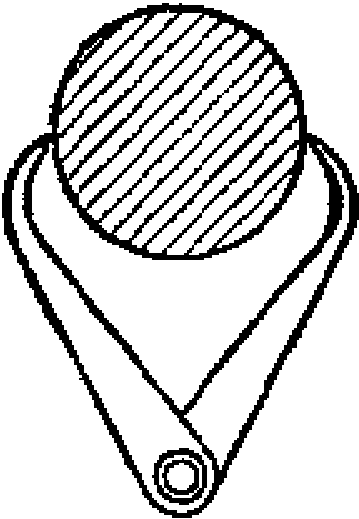
\includegraphics[width=2.5cm]{../pic/czjh2-ch7-xiti24-01.png}
        \caption*{(第 1 题)}
    \end{minipage}
    \qquad
    \begin{minipage}[b]{4cm}
        \centering
        \begin{tikzpicture}
    \tkzDefPoints{0/0/O}
    \tkzDefPoint(200:1.5){A}
    \tkzDefPoint(20:1.5){B}
    \tkzDefPoint(235:1.5){C}
    \tkzDefPoint(305:1.5){D}
    \tkzDefLine[altitude](C,A,D)  \tkzGetPoint{E}
    \tkzDefLine[altitude](C,B,D)  \tkzGetPoint{F}

    \tkzDrawCircle[thick](O,A)
    \tkzDrawSegments(A,B  A,E  B,F)
    \tkzDrawLine[add=0.1 and 0.1](E,F)
    \tkzDrawPoint(O)
    \tkzMarkRightAngle[size=.2](A,E,C)
    \tkzMarkRightAngle[size=.2](B,F,D)
    \tkzLabelPoints[above](O)
    \tkzLabelPoints[left](A)
    \tkzLabelPoints[right](B)
    \tkzLabelPoints[below](C)
    \tkzLabelPoints[below](D)
    \tkzLabelPoints[below left](E)
    \tkzLabelPoints[below right](F)
\end{tikzpicture}


        \caption*{(第 8 题)}
    \end{minipage}
    \qquad
    \begin{minipage}[b]{5cm}
        \centering
        \begin{tikzpicture}
    \pgfmathsetmacro{\factor}{0.025}
    \pgfmathsetmacro{\R}{130*\factor/2}
    \tkzDefPoints{0/0/O}
    \tkzDefPoint(180:\R){C}
    \tkzDefPoint(0:\R){D}
    \tkzDefPoint(90:\R){E}
    \tkzDefPointOnLine[pos=32/65](O,E)  \tkzGetPoint{F}
    \tkzDefLine[parallel=through F](C,D)  \tkzGetPoint{a}
    \tkzInterLC(F,a)(O,C)  \tkzGetPoints{B}{A}

    \tkzDrawCircle[thick](O,A)
    \tkzDrawArc[pattern={mylines[angle=65, distance={4pt}]}](O,B)(A)
    \tkzDrawSegments(A,B)
    \tkzDrawSegment[latex-latex](C,D)  \tkzLabelSegment[below](C,D){$\phi 130$}
    \tkzDrawPoint(O)

    \tkzLabelPoints[above](O)
    \tkzLabelPoints[left](A)
    \tkzLabelPoints[above, xshift=.5em](B)

    %
    \tkzDefPointOnLine[pos=1.4](F,B)  \tkzGetPoint{G}
    \tkzDefPointBy[translation=from F to G](E)  \tkzGetPoint{H}
    \tkzDefShiftPoint[G](0,-0.4){g}
    \tkzDefShiftPoint[H](0, 0.4){h}
    \tkzDrawLines[add=0 and 0.1](E,H  F,G)
    \tkzLabelSegment[rotate=90, yshift=.5em](G,H){$32$}  \tkzDrawSegments[-latex](g,G  h,H)
\end{tikzpicture}


        \caption*{(第 9 题)}
    \end{minipage}
    \qquad
\end{figure}

\xiaoti{如图,$AB$ 是 $\yuan\,O$ 的直径, $CD$ 是弦, $AE \perp CD$,垂足为 $E$;
    $BF \perp CD$, 垂足为 $F$。 求证: $EC = FD$。
}

\xiaoti{在直径为 130 mm 的圆铁片上切去一块高为 32 mm 的弓形铁片(如图)。
    求弓形的弦 $AB$ 的长。
}

\xiaoti{破残的轮片上,弓形的弦 $AB$ 长 480 mm, 高 $CD$ 为 70 mm(如图)。求原轮片的直径。}

\begin{figure}[htbp]
    \centering
    \begin{minipage}[b]{7cm}
        \centering
        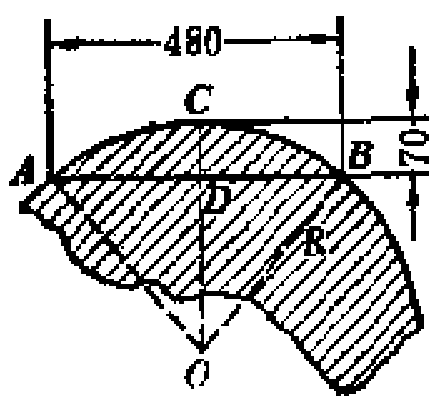
\includegraphics[width=4cm]{../pic/czjh2-ch7-xiti24-10.png}
        \caption*{(第 10 题)}
    \end{minipage}
    \qquad
    \begin{minipage}[b]{4cm}
        \centering
        \begin{tikzpicture}
    \tkzDefPoints{0/0/B, 2.5/0.5/C}
    \tkzDefTriangle[equilateral](B,C)  \tkzGetPoint{A}
    \tkzDefCircle[circum](A,B,C)  \tkzGetPoints{O}{R}
    \tkzDefTriangle[two angles=80 and 40](B,C)  \tkzGetPoint{P}

    \tkzDrawCircle[thick](O,R)
    \tkzDrawPolygon(A,P,B,C)
    \tkzDrawSegments(A,B  C,P)
    \tkzDrawPoint(O)
    \tkzLabelPoints[below](O)
    \tkzLabelPoints[above](A)
    \tkzLabelPoints[left](B)
    \tkzLabelPoints[right](C)
    \tkzLabelPoints[above](P)
\end{tikzpicture}


        \caption*{(第 14 题)}
    \end{minipage}
\end{figure}

\xiaoti{弦 $AB$ 和 $CD$ 相交于圆内的点 $P$,并且和经过点 $P$ 的直径成等角。求证: $AB = CD$。}

\xiaoti{}%
\begin{xiaoxiaotis}%
    \xxt[\xxtsep]{求证:经过 $\yuan\,O$ 内一点 $P$ 的所有弦中,与 $OP$ 垂直的弦最短;}

    \xxt{已知 $\yuan\,O$ 的半径为 6 厘米, $OP = 3.6$ 厘米。求经过点 $P$ 最短的弦长。}

\end{xiaoxiaotis}

\xiaoti{圆内接六边形 $ABCDEF$ 的各边相等,求各边所对的圆心角的度数。}

\xiaoti{已知:如图, $\angle APC = \angle CPB = 60^\circ$。
    求证: $\triangle ABC$ 是等边三角形。
}

\xiaoti{圆上一点 $P$ 到直径 $AB$ 的垂线的垂足为 $D$。求证: $\triangle BPD \xiangsi \triangle PAD$。}

\xiaoti{$\triangle ABC$ 中, $\angle BAC$ 的平分线与边 $BC$ 和外接圆分别相交于点 $D$ 和 $E$。
    求证: $\triangle ABD \xiangsi \triangle AEC$。
}

\xiaoti{求证:以等腰三角形的一腰为直径的圆,平分底边。}

\xiaoti{圆内接三角形 $ABC$ 中, $AB = AC$, 经过点 $A$ 的弦与 $BC$ 和 $\yuanhu{BC}$
    分别相交于点 $D$ 和 $E$。 求证: $\triangle ABD \xiangsi \triangle AEB$。
}

\xiaoti{使用曲尺检验工件的凹面,成半圆形时为合格。如图所示的三种情况中,
    哪种是合格的?哪种是不合格的?为什么?
}

\begin{figure}[htbp]
    \centering
    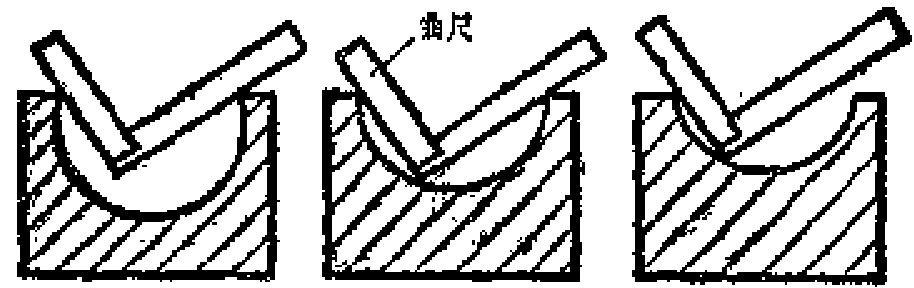
\includegraphics[width=8cm]{../pic/czjh2-ch7-xiti24-19.png}
    \caption*{(第 19 题)}
\end{figure}

\xiaoti{已知线段 $AB$ ,怎样作出几个点 $C_1$、$C_2$、…,使它们对 $AB$ 所张的角
    $\angle AC_1B$、$\angle AC_2B$、… 都是直角?
}

\xiaoti{圆内接四边形 $ABCD$ 中, $\angle A$、$\angle B$、$\angle C$ 的度数的比是 $2:3:6$。求四边形各内角的度数。}

\xiaoti{如图, $AD$ 是 $\triangle ABC$ 外角 $\angle EAC$ 的平分线,与三角形的外接圆交于点 $D$。求证: $DB = DC$。}

\begin{figure}[htbp]
    \centering
    \begin{minipage}[b]{5cm}
        \centering
        \begin{tikzpicture}
    \tkzDefPoints{0/0/O}
    \tkzDefPoint(120:1.5){A}
    \tkzDefPoint(225:1.5){B}
    \tkzDefPoint(315:1.5){C}
    \tkzDefPointOnLine[pos=1.4](B,A)  \tkzGetPoint{E}
    \tkzDefLine[bisector](C,A,E)  \tkzGetPoint{d}
    \tkzInterLC[common=A](A,d)(O,A)  \tkzGetFirstPoint{D}

    \tkzDrawCircle[thick](O,A)
    \tkzDrawPolygon(A,B,C)
    \tkzDrawSegments(A,C  A,D  A,E  B,D  C,D)
    \tkzLabelPoints[left, yshift=.5em](A)
    \tkzLabelPoints[left](B)
    \tkzLabelPoints[right](C)
    \tkzLabelPoints[above](D)
    \tkzLabelPoints[left](E)
\end{tikzpicture}


        \caption*{(第 22 题)}
    \end{minipage}
    \qquad
    \begin{minipage}[b]{6cm}
        \centering
        \begin{tikzpicture}
    \tkzDefPoints{0/0/B, 4/0/C, 1/2.5/A}
    \tkzDefLine[altitude](A,B,C)  \tkzGetPoint{E}
    \tkzDefLine[altitude](A,C,B)  \tkzGetPoint{F}

    \tkzDrawPolygon(A,B,C)
    \tkzDrawSegments(B,E  C,F  E,F)
    \tkzMarkRightAngle[size=.2](B,E,C)
    \tkzMarkRightAngle[size=.2](B,F,C)
    \tkzLabelPoints[above](A)
    \tkzLabelPoints[left](B,F)
    \tkzLabelPoints[right](C,E)
\end{tikzpicture}


        \caption*{(第 23 题)}
    \end{minipage}
\end{figure}

\xiaoti{已知: $BE$、$CF$ 是 $\triangle ABC$ 的两条高。 求证: $\angle AEF = \angle ABC$。}

\xiaoti{用反证法证明:}
\begin{xiaoxiaotis}

    \xxt{一个三角形的内角中,不能有两个钝角或直角;}

    \xxt{在同圆内,如果两条弦不等,那么它们的弦心距也不等;}

    \xxt{在同一平面内,一条直线与两条平行线中的一条相交,必定与另一条也相交。}

\end{xiaoxiaotis}



\end{xiaotis}



\section{直线和圆的位置关系}
\subsection{直线和圆的位置关系}\label{subsec:czjh2-7-7}

在黑板上画一个圆,把直尺当做一条直线在黑板面上移动。我们可以看到,直线和圆的位置关系有下面三种。

\begin{figure}[htbp]
    \centering
    \begin{minipage}[b]{4.5cm}
        \centering
        \begin{tikzpicture}
    \tkzDefPoints{0/0/O}
    \tkzDefPoint(0:1.5){A}
    \tkzDefPoint(270:1.8){P}
    \tkzDefLine[perpendicular=through P,normed](O,P)  \tkzGetPoint{q}
    \tkzDefPointOnLine[pos=2.0](P,q)  \tkzGetPoint{Q}

    \tkzDrawCircle[thick](O,A)
    \tkzDrawPoint(O)
    \tkzDrawSegment(O,P)
    \tkzDrawLine[add=0 and 1](Q,P)
    \tkzMarkRightAngle[size=.2](O,P,Q)
    \tkzLabelPoints[above](O)
    \tkzLabelPoints[below](P)
    \tkzLabelSegment[pos=1, right](P,Q){$l$}
\end{tikzpicture}


        \caption*{甲}
    \end{minipage}
    \qquad
    \begin{minipage}[b]{4.5cm}
        \centering
        \begin{tikzpicture}
    \tkzDefPoints{0/0/O}
    \tkzDefPoint(0:1.5){A}
    \tkzDefPoint(270:1.5){P}
    \tkzDefLine[perpendicular=through P,normed](O,P)  \tkzGetPoint{q}
    \tkzDefPointOnLine[pos=2.0](P,q)  \tkzGetPoint{Q}

    \tkzDrawCircle[thick](O,A)
    \tkzDrawPoint(O)
    \tkzDrawSegment(O,P)
    \tkzDrawLine[add=0 and 1](Q,P)
    \tkzMarkRightAngle[size=.2](O,P,Q)
    \tkzLabelPoints[above](O)
    \tkzLabelPoints[below](P)
    \tkzLabelSegment[pos=1, right](P,Q){$l$}

    % 通过显示一个无色的 "P",实现三张图片的 “圆点” 在同一水平线。
    \tkzDefPoint(270:1.8){P}
    \tkzLabelPoints[below,transparent](P)
\end{tikzpicture}


        \caption*{乙}
    \end{minipage}
    \qquad
    \begin{minipage}[b]{4.5cm}
        \centering
        \begin{tikzpicture}
    \tkzDefPoints{0/0/O}
    \tkzDefPoint(0:1.5){A}
    \tkzDefPoint(270:1.0){P}
    \tkzDefLine[perpendicular=through P,normed](O,P)  \tkzGetPoint{q}
    \tkzDefPointOnLine[pos=2.0](P,q)  \tkzGetPoint{Q}

    \tkzDrawCircle[thick](O,A)
    \tkzDrawPoint(O)
    \tkzDrawSegment(O,P)
    \tkzDrawLine[add=0 and 1](Q,P)
    \tkzMarkRightAngle[size=.2](O,P,Q)
    \tkzLabelPoints[above](O)
    \tkzLabelPoints[below](P)
    \tkzLabelSegment[pos=1, right](P,Q){$l$}

    % 通过显示一个无色的 "P",实现三张图片的 “圆点” 在同一水平线。
    \tkzDefPoint(270:1.8){P}
    \tkzLabelPoints[below,transparent](P)
\end{tikzpicture}


        \caption*{丙}
    \end{minipage}
    \caption{}\label{fig:czjh2-7-32}
\end{figure}

(1)直线和圆没有公共点时,叫做直线和圆\zhongdian{相离}(图 \ref{fig:czjh2-7-32} 甲)。

(2)直线和圆有唯一公共点时,叫做直线和圆\zhongdian{相切}(图 \ref{fig:czjh2-7-32} 乙)。
这时直线叫做圆的\zhongdian{切线},唯一的公共点叫做\zhongdian{切点}。

(3)直线和圆有两个公共点时,叫做直线和圆\zhongdian{相交}(图 \ref{fig:czjh2-7-32} 丙)。
这时直线叫做圆的\zhongdian{割线}。

根据直线与圆相离、相切、相交的定义,容易看出:

如果 $\yuan\,O$ 的半径为 $r$, 圆心 $O$ 到直线 $l$ 的距离为 $d$,那么


\zhongdian{(1) 直线 $\bm{l}$ 和 $\bm{\yuan\,O}$ 相离 $\dengjiayu \bm{d > r}$;}

\zhongdian{(2) 直线 $\bm{l}$ 和 $\bm{\yuan\,O}$ 相切 $\dengjiayu \bm{d = r}$;}

\zhongdian{(3) 直线 $\bm{l}$ 和 $\bm{\yuan\,O}$ 相交 $\dengjiayu \bm{d < r}$。}


\begin{lianxi}

已知 $Rt \triangle ABC$ 的斜边 $AB = 6$ cm,直角边 $AC = 3$ cm。
圆心为 $C$,半径分别为 $2$ cm, $4$ cm 的两个圆与 $AB$ 有怎样的位置关系?
半径多长时, $AB$ 与圆相切?

\end{lianxi}


\subsection{切线的判定和性质}\label{subsec:czjh2-7-8}

如图 \ref{fig:czjh2-7-33},在 $\yuan\,O$ 中,经过半径 $OA$ 的外端点 $A$,作直线 $l \perp OA$,
则圆心 $O$ 与直线 $l$ 的距离就是半径 $r$。由上一节我们知道,这样的直线与圆一定相切。
因此有下面定理:

\begin{dingli}[切线的判定定理]
    经过半径的外端并且垂直于这条半径的直线是圆的切线。
\end{dingli}

\begin{figure}[htbp]
    \centering
    \begin{minipage}[b]{7cm}
        \centering
        \begin{tikzpicture}
    \tkzDefPoints{0/0/O}
    \tkzDefPoint(270:1.5){A}
    \tkzDefLine[perpendicular=through A,normed](O,A)  \tkzGetPoint{b}
    \tkzDefPointOnLine[pos=2.0](A,b)  \tkzGetPoint{B}

    \tkzDrawCircle[thick](O,A)
    \tkzDrawPoint(O)
    \tkzDrawSegment(O,A)
    \tkzDrawLine[add=0 and 1](B,A)
    \tkzMarkRightAngle[size=.2](O,A,B)
    \tkzLabelPoints[above](O)
    \tkzLabelPoints[below](A)
    \tkzLabelSegment[pos=1, right](A,B){$l$}
\end{tikzpicture}


        \caption{}\label{fig:czjh2-7-33}
    \end{minipage}
    \qquad
    \begin{minipage}[b]{7cm}
        \centering
        \begin{tikzpicture}
    \tkzDefPoints{0/0/O}
    \tkzDefPoint(270:1.5){C}
    \tkzDefLine[perpendicular=through C,normed](O,C)  \tkzGetPoint{b}
    \tkzDefPointOnLine[pos=2.0](C,b)  \tkzGetPoint{B}
    \tkzDefPointOnLine[pos=2](B,C)  \tkzGetPoint{A}

    \tkzDrawCircle[thick](O,C)
    \tkzDrawPoint(O)
    \tkzDrawSegment[dashed](O,C)
    \tkzDrawSegments(O,A  O,B)
    \tkzDrawLine[add=.1 and .1](A,B)
    \tkzLabelPoints[above](O)
    \tkzLabelPoints[below](A,B,C)
\end{tikzpicture}


        \caption{}\label{fig:czjh2-7-34}
    \end{minipage}
\end{figure}

\liti 已知:直线 $AB$ 经过 $\yuan\,O$ 上的点 $C$, 并且 $OA = OB$,$CA = CB$(图 \ref{fig:czjh2-7-34})。

求证: 直线 $AB$ 是 $\yuan\,O$ 的切线。

\zhengming 连结 $OC$。

$\because$ \quad $OA = OB$, $CA = CB$,

$\therefore$ \quad $OC$ 是等腰三角形 $OAB$ 底边 $AB$ 上的中线。

$\therefore$ \quad $AB \perp OC$。

因此,直线 $AB$ 经过半径 $OC$ 的外端 $C$,并且垂直于半径 $OC$, 所以 $AB$ 是 $\yuan\,O$ 的切线。


\begin{dingli}[切线的性质定理]
    圆的切线垂直于经过切点的半径。
\end{dingli}


已知: 如图 \ref{fig:czjh2-7-35},直线 $AT$ 是 $\yuan\,O$ 的切线, $A$ 为切点。

求证: $AT \perp OA$。

\zhengming 假设 $AT$ 与 $0A$ 不垂直。

经过圆心且垂直于切线的直线必经过

过圆心 $O$ 作 $OM \perp AT$, 交 $AT$ 于点 $M$。由垂线段最短,得 $OM < OA$。

因为圆心到直线 $AT$ 的距离小于半径,所以 $AT$ 与 $\yuan\,O$ 相交。 这与已知相矛盾。

$\therefore$ \quad $AT \perp OA$。


由于过已知点只有一条直线与已知直线垂直, 所以经过圆心垂直于切线的直线一定过切点;
反过来,过切点垂直于切线的直线也一定经过圆心。 由此得到:

\begin{tuilun}[推论1]
    经过圆心且垂直于切线的直线必经过切点。
\end{tuilun}

\begin{tuilun}[推论2]
    经过切点且垂直于切线的直线必经过圆心。
\end{tuilun}

\begin{figure}[htbp]
    \centering
    \begin{minipage}[b]{7cm}
        \centering
        \begin{tikzpicture}
    \tkzDefPoints{0/0/O}
    \tkzDefPoint(270:1.5){A}
    \tkzDefLine[perpendicular=through A,normed](O,A)  \tkzGetPoint{T}
    \tkzDefPointOnLine[pos=2.0](A,T)  \tkzGetPoint{T}
    \tkzDefPointOnLine[pos=.4](A,T)  \tkzGetPoint{M}

    \tkzDrawCircle[thick](O,A)
    \tkzDrawPoint(O)
    \tkzDrawSegment(O,A)
    \tkzDrawLine[add=0 and 1](T,A)
    \tkzDrawSegment[dashed](O,M)
    \tkzLabelPoints[above](O)
    \tkzLabelPoints[below](A,M)
    \tkzLabelPoints[right](T)
\end{tikzpicture}


        \caption{}\label{fig:czjh2-7-35}
    \end{minipage}
    \qquad
    \begin{minipage}[b]{7cm}
        \centering
        \begin{tikzpicture}
    \tkzDefPoints{0/0/O}
    \tkzDefPoint(180:1.5){A}
    \tkzDefPoint(0:1.5){B}
    \tkzDefLine[perpendicular=through B,normed](O,B)  \tkzGetPoint{c}
    \tkzDefPointOnLine[pos=2.0](B,c)  \tkzGetPoint{C}
    \tkzDefLine[parallel=through A](O,C)  \tkzGetPoint{d}
    \tkzInterLC[common=A](A,d)(O,A)  \tkzGetFirstPoint{D}

    \tkzDrawCircle[thick](O,A)
    \tkzDrawSegments(A,B  A,D  O,C)
    \tkzDrawLine[add=0 and .7](C,B)
    \tkzDrawLine[add=0 and .7](C,D)
    \tkzDrawSegment[dashed](O,D)
    \extkzLabelAngel[0.4](O,A,D){$1$}
    \extkzLabelAngel[0.4](A,D,O){$2$}
    \extkzLabelAngel[0.5](B,O,C){$3$}
    \extkzLabelAngel[0.4](C,O,D){$4$}
    \tkzLabelPoints[below](O)
    \tkzLabelPoints[left](A)
    \tkzLabelPoints[right](B,C)
    \tkzLabelPoints[above](D)
\end{tikzpicture}


        \caption{}\label{fig:czjh2-7-36}
    \end{minipage}
\end{figure}


\liti 已知: $AB$ 是 $\yuan\,O$ 的直径, $BC$ 是 $\yuan\,O$ 的切线,切点为 $B$,
$OC$ 平行于弦 $AD$ (图 \ref{fig:czjh2-7-36})。

求证: $DC$ 是 $\yuan\,O$ 的切线。

\zhengming 连结 $OD$。

$\left.\begin{aligned}
    OA = OD          \tuichu  \angle 1 = \angle 2 \\
    AD \pingxing OC  \tuichu  \left\{\begin{aligned}
        \angle 1 = \angle 3 \\
        \angle 2 = \angle 4
    \end{aligned}\right\}
\end{aligned}\right\}  \tuichu  \angle 3 = \angle 4 \juhao$

$\left.\begin{aligned}
    OB = OD \\
    \angle 3 = \angle 4 \\
    OC = OC
\end{aligned}\right\}  \tuichu  \triangle OBC \quandeng \triangle ODC  \tuichu  \angle OBC = \angle ODC \juhao$


$\because$ \quad $BC$ 是 $\yuan\,O$ 的切线,

$\therefore$ \quad $\angle OBC = 90^\circ$。

$\therefore$ \quad $\angle ODC = 90^\circ$。

$\therefore$ \quad $DC$ 是 $\yuan\,O$ 的切线。



\begin{lianxi}

\xiaoti{如图, $AB$ 是 $\yuan\,O$ 的直径, $\angle ABT = 45^\circ$, $AT = AB$。
    求证: $AT$ 是 $\yuan\,O$ 的切线。
}

\begin{figure}[htbp]
    \centering
    \begin{minipage}[b]{4.8cm}
        \centering
        \begin{tikzpicture}
    \tkzDefPoints{0/0/O}
    \tkzDefPoint(270:1.5){A}
    \tkzDefPoint(90:1.5){B}
    \tkzDefTriangle[two angles=90 and 45](A,B)  \tkzGetPoint{T}

    \tkzDrawCircle[thick](O,A)
    \tkzDrawPolygon(A,B,T)
    \tkzDrawPoint(O)
    \tkzMarkAngle[size=.5](T,B,A)
    \tkzLabelPoints[right](O)
    \tkzLabelPoints[below](A)
    \tkzLabelPoints[above](B)
    \tkzLabelPoints[below](T)
\end{tikzpicture}


        \caption*{(第 1 题)}
    \end{minipage}
    \qquad
    \begin{minipage}[b]{5.2cm}
        \centering
        \begin{tikzpicture}
    \tkzDefPoints{0/0/O}
    \tkzDefPoint(180:1.5){A}
    \tkzDefPoint(0:1.5){B}
    \tkzDefPointOnLine[pos=2](O,B)  \tkzGetPoint{D}
    \tkzDefPoint(60:1.5){C}  % OD = 2OC, 再根据结论:DC 是切线,角OCD = 90度,所以,角 CDO = 30 度,即:角 DOC = 60 度

    \tkzDrawCircle[thick](O,A)
    \tkzDrawPoint(O)
    \tkzDrawSegments(A,C  A,D)
    \tkzDrawLine[add=0 and 0.6](D,C)
    \tkzLabelPoints[below](O)
    \tkzLabelPoints[left](A)
    \tkzLabelPoints[below,xshift=.5em](B)
    \tkzLabelPoints[above](C)
    \tkzLabelPoints[below,xshift=-.5em](D)
\end{tikzpicture}


        \caption*{(第 2 题)}
    \end{minipage}
    \qquad
    \begin{minipage}[b]{4.5cm}
        \centering
        \begin{tikzpicture}
    \tkzDefPoints{0/0/O}
    \tkzDefPoint(70:3.5){A}
    \tkzDefPoint(0:3.5){B}
    \tkzDefPoint(35:4.5){C}
    \tkzDefPointOnLine[pos=.55](O,C)  \tkzGetPoint{D}
    \tkzDefLine[altitude](A,D,O)  \tkzGetPoint{E}

    \tkzDrawCircle[thick](D,E)
    \tkzDrawPoint(D)
    \tkzDrawSegments(O,A  O,B  O,C)
    \tkzLabelPoints[below](O)
    \tkzLabelPoints[left](A)
    \tkzLabelPoints[below](B)
    \tkzLabelPoints[below](C)
    \tkzLabelPoints[above left](D)
    \tkzLabelPoints[left](E)
\end{tikzpicture}


        \caption*{(第 4 题)}
    \end{minipage}
\end{figure}

\xiaoti{$AB$ 是 $\yuan\,O$ 的直径,点 $D$ 在 $AB$ 的延长线上, $BD = OB$,点 $C$ 在圆上,
    $\angle CAB = 30^\circ$。 求证: $DC$ 是 $\yuan\,O$ 的切线。
}

\xiaoti{求证:}
\begin{xiaoxiaotis}

    \xxt{经过圆的直径两端点的切线互相平行;}

    \xxt{圆的两条切线互相平行,则连结两个切点的线段是直径。}

\end{xiaoxiaotis}


\xiaoti{已知: $OC$ 平分 $\angle AOB$, $D$ 是 $OC$ 上任意一点,
    $\yuan\,D$ 与 $OA$ 相切于点 $E$。 求证: $OB$ 与 $\yuan\,D$ 相切。
}

\end{lianxi}

\subsection{圆的切线的作法,切线长定理}\label{subsec:czjh2-7-9}

根据切线的判定定理,可以得到经过一个已知点作已知圆的切线的方法。
分已知点在圆上与圆外两种情况说明如下:

(1)已知:$\yuan\,O$ 及 $\yuan\,O$ 上的一点 $P$ (图 \ref{fig:czjh2-7-37})。

求作:经过点 $P$ 的 $\yuan\,O$ 的切线。

\zuofa 1. 连结 $OP$。

2. 经过点 $P$ 作 $BC \perp OP$。

直线 $BC$ 就是所求的切线。

由作法可以知道,经过 $\yuan\,O$ 上的一点 $P$,
可以作出并且只可以作出一条 $\yuan\,O$ 的切线。

\begin{figure}[htbp]
    \centering
    \begin{minipage}[b]{7cm}
        \centering
        \begin{tikzpicture}
    \tkzDefPoints{0/0/O}
    \tkzDefPoint(0:1.5){P}
    \tkzDefLine[perpendicular=through P,normed](O,P)  \tkzGetPoint{b}
    \tkzDefPointOnLine[pos=2.0](P,b)  \tkzGetPoint{B}
    \tkzDefPointOnLine[pos=2.0](B,P)  \tkzGetPoint{C}

    \tkzDrawCircle[thick](O,P)
    \tkzDrawPoint(O)
    \tkzDrawSegments(O,P  B,C)
    \tkzLabelPoints[left](O)
    \tkzLabelPoints[right](B,C,P)
\end{tikzpicture}


        \caption{}\label{fig:czjh2-7-37}
    \end{minipage}
    \qquad
    \begin{minipage}[b]{7cm}
        \centering
        \begin{tikzpicture}
    \tkzDefPoints{0/0/O, 1.1/0/R, 3/0/P}
    \tkzDrawCircle[thick](O,R)
    \tkzLabelPoints[left](O)
    \tkzLabelPoints[below=.2em, xshift=.3em](P)

    % 1
    \tkzDrawSegment(O,P)

    % 2
    \tkzDefMidPoint(O,P)  \tkzGetPoint{C}
    \tkzDrawCircle[thick](C,O)
    \tkzDrawPoint(C)
    \tkzInterCC(O,R)(C,O)  \tkzGetPoints{A}{B}
    \tkzLabelPoints[above, xshift=-.2em](A)
    \tkzLabelPoints[below, xshift=-.2em](B)
    \tkzLabelPoints[below](C)

    % 3
    \tkzDrawLines[add=0.2 and 0.2](P,A  P,B)
    \tkzDrawSegments[dashed](O,A  O,B)
\end{tikzpicture}


        \caption{}\label{fig:czjh2-7-38}
    \end{minipage}
\end{figure}

(2)已知: $\yuan\,O$ 及 $\yuan\,O$ 外的一点 $P$(图 \ref{fig:czjh2-7-38})。

求作:经过点 $P$ 的 $\yuan\,O$ 的切线。

分析: 设 $PA$ 是经过点 $P$ 和 $\yuan\,O$ 相切于点 $A$ 的直线,由切线的性质定理,
可知 $OA \perp AP$, 点 $A$ 必在以 $OP$ 为直径的圆上。

\zuofa 1. 连结 $OP$。

2. 以 $OP$ 为直径作 $\yuan\,C$, $\yuan\,C$ 和 $\yuan\,O$ 相交干两点 $A$、$B$。

3. 作直线 $PA$、$PB$。

直线 $PA$、$PB$ 就是所求的切线。

\zhengming 连结 $OA$、$OB$。

$\because$ \quad $OP$ 是 $\yuan\,C$ 的直径,

$\therefore$ \quad $\angle OAP$、$\angle OBP$ 都是直角。

因此, $PA$、$PB$ 是 $\yuan\,O$ 的切线。

由作法可以知道, 经过 $\yuan\,O$ 外的一点 $P$, 可以作出 $\yuan\,O$ 的两条切线。

在经过圆外一点的切线上, 这一点和切点之间的线段的长叫做这点到圆的\zhongdian{切线长}。

在图 \ref{fig:czjh2-7-38} 中,

$\because$ \quad $OA = OB$, $OP = OP$,

$\therefore$ \quad $Rt \triangle AOP \quandeng Rt \triangle BOP$。

$\therefore$ \quad $PA = PB$, $\angle OPA = \angle OPB$。

由此得到下面的定理:

\begin{dingli}[切线长定理]
    从圆外一点引圆的两条切线,它们的切线长相等,圆心和这一点的连线平分两条切线的夹角。
\end{dingli}



\begin{lianxi}

\xiaoti{作已知圆的切线,使它:}
\begin{xiaoxiaotis}

    \xxt{和一条已知直线平行;}

    \xxt{和一条已知直线垂直。}

\end{xiaoxiaotis}


\xiaoti{已知: $\yuan\,O$ 的半径为 3 厘米, 点 $P$ 和圆心 $O$ 的距离为 6 厘米。}
\begin{xiaoxiaotis}

    \xxt{经在点 $P$ 作 $\yuan\,O$ 的切线;}

    \xxt{求两条切线的夹角及切线长。}
\end{xiaoxiaotis}

\xiaoti{$PA$ 和 $PB$ 是 $\yuan\,O$ 的切线, $A$ 和 $B$ 是切点。
    求证: $OP$ 垂直平分弦 $AB$。
}

\end{lianxi}


\subsection{三角形的内切圆}\label{subsec:czjh2-7-10}

从一块三角形的材料上裁下一块圆形的用料,怎样才能使圆的半径尽可能大呢?这实际是下面的问题。

\zhongdian{作圆,使它和已知三角形的各边都相切。}

已知: $\triangle ABC$ (图 \ref{fig:czjh2-7-39})。

求作: 和 $\triangle ABC$ 的各边都相切的圆。

分析:要作一个圆与  $\triangle ABC$ 三边都相切,就是要求出一点作为圆心,使它到三边的距离相等。
以前我们学过三角形三个内角的平分线相交于一点,这一点到三边的距离相等。由此可得三角形内切圆的作法。

\zuofa 1. 作 $\angle B$、$\angle C$ 的平分线 $BM$ 和 $CN$,交点为 $I$。

2. 过点 $I$ 作 $ID \perp BC$,垂足为 $D$。

3. 以 $I$ 为圆心, $ID$ 为半径作 $\yuan\,I$。

$\yuan\,I$ 就是所求的圆。

\zhengming 过点 $I$ 分别作 $CA$、$AB$ 的垂线,垂足为 $E$、$F$。

$\because$ \quad  $I$ 在 $\angle ABC$、$\angle ACB$ 的平分线上,

$\therefore$ \quad $IF = ID$,$IE = ID$。

$\therefore$ \quad $D$、$E$、$F$ 都在 $\yuan\,I$ 上。

又因为 $BC$、$CA$、$AB$ 经过点 $D$、$E$、$F$, 且 $BC \perp ID$、$CA \perp IE$、$AB \perp IF$,
所以 $\triangle ABC$ 的三边 $BC$、$CA$、$AB$ 都与 $\yuan\,I$ 相切。

因为三角形的三条角平分线有一个且只有一个交点,所以,
和三角形的各边都相切的圆可以作出一个且只可以作出一个。

和三角形各边都相切的圆叫做\zhongdian{三角形的内切圆},
内切圆的圆心叫做三角形的\zhongdian{内心},
这个三角形叫做\zhongdian{圆的外切三角形}。

一般地,和多边形的各边都相切的圆叫做\zhongdian{多边形的内切圆},
这个多边形叫做\zhongdian{圆的外切多边形}。

\begin{figure}[htbp]
    \centering
    \begin{minipage}[b]{7cm}
        \centering
        \begin{tikzpicture}
    \tkzDefPoints{0/0/B, 4/0/C, 3.5/2.5/A}
    \tkzDrawPolygon(A,B,C)
    \tkzLabelPoints[above](A)
    \tkzLabelPoints[left](B)
    \tkzLabelPoints[right](C)

    % 1
    \tkzDefLine[bisector](C,B,A)  \tkzGetPoint{M}
    \tkzDefLine[bisector](A,C,B)  \tkzGetPoint{N}
    \tkzInterLL(B,M)(C,N)  \tkzGetPoint{I}
    \tkzDrawSegments(B,M  C,N)
    \tkzLabelPoints[above](I)
    \tkzLabelPoints[left,yshift=.5em](M)
    \tkzLabelPoints[left,xshift=.3em](N)

    % 2
    \tkzDefLine[altitude](B,I,C)  \tkzGetPoint{D}
    \tkzDrawSegment(I,D)
    \tkzMarkRightAngle[size=.2](I,D,B)
    \tkzLabelPoints[below](D)

    % 3
    \tkzDrawCircle[thick](I,D)

    % 证明
    \tkzDefLine[altitude](C,I,A)  \tkzGetPoint{E}
    \tkzDefLine[altitude](A,I,B)  \tkzGetPoint{F}
    \tkzDrawSegments[dashed](I,E  I,F)
    \tkzLabelPoints[right](E)
    \tkzLabelPoints[above left](F)
\end{tikzpicture}


        \caption{}\label{fig:czjh2-7-39}
    \end{minipage}
    \qquad
    \begin{minipage}[b]{7cm}
        \centering
        \begin{tikzpicture}
    % 圆的外切四边形的两组对边的和相等
    % AB + CD  = AD  + BC
    % 4  + 2.5 = 3.5 + 3
    \tkzDefPoints{0/0/A, 4/0/B}
    \tkzDefPoint(70:3.5){D}
    \tkzInterCC[R](D,2.5)(B,3)  \tkzGetFirstPoint{C}

    % 切线长定理
    \tkzDefLine[bisector](B,A,D)  \tkzGetPoint{a}
    \tkzDefLine[bisector](C,B,A)  \tkzGetPoint{b}
    \tkzInterLL(A,a)(B,b)  \tkzGetPoint{O}
    \tkzDefLine[altitude](A,O,B)  \tkzGetPoint{L}
    \tkzDefLine[altitude](B,O,C)  \tkzGetPoint{M}
    \tkzDefLine[altitude](C,O,D)  \tkzGetPoint{N}
    \tkzDefLine[altitude](D,O,A)  \tkzGetPoint{P}

    \tkzDrawPolygon(A,B,C,D)
    \tkzDrawCircle[thick](O,L)
    \tkzDrawPoint(O)
    \tkzLabelPoints[left](A,D,P)
    \tkzLabelPoints[right](B,C,M)
    \tkzLabelPoints[above](N)
    \tkzLabelPoints[below](L,O)
\end{tikzpicture}


        \caption{}\label{fig:czjh2-7-40}
    \end{minipage}
\end{figure}

图 \ref{fig:czjh2-7-40} 中, $\yuan\,O$ 是四边形 $ABCD$ 的内切圆,四边形 $ABCD$ 是 $\yuan\,O$ 的外切四边形。


\liti[0] \zhongdian{圆的外切四边形的两组对边的和相等。}

已知:四边形 $ABCD$ 的边 $AB$、$BC$、$CD$、$DA$ 和 $\yuan\,O$
分别相切于点 $L$、$M$、$N$、$P$(图 \ref{fig:czjh2-7-40})。

求证: $AB + CD = AD + BC$。

证明: 因为 $AB$、$BC$、$CD$、$DA$ 都与 $\yuan\,O$ 相切,$L$、$M$、$N$、$P$ 是切点,

$\therefore$ \quad $AL = AP$, $LB = MB$, $DN = DP$, $NC = MC$。

$\therefore$ \quad $\begin{aligned}[t]
      & AL + LB + DN + NC \\
    = & AP + MB + DP + MC \\
    = & AP + DP + MB + MC \douhao
\end{aligned}$

即 \quad $AB + CD = AD + BC$。


\begin{lianxi}

\xiaoti{设 $\triangle ABC$ 的内切圆 $I$ 和各边分别相切于点 $D$、$E$、$F$,
    $\angle DIE = 118^\circ$, $\angle FID = 144^\circ$。
    求 $\triangle ABC$ 各内角的度数。
}

\begin{figure}[htbp]
    \centering
    \begin{minipage}[b]{5.6cm}
        \centering
        \begin{tikzpicture}
    \tkzDefPoints{0/0/B, 5/0/C}
    \tkzDefTriangle[two angles=36 and 62](B,C)  \tkzGetPoint{A}
    \tkzDefLine[bisector](B,A,C)  \tkzGetPoint{a}
    \tkzDefLine[bisector](C,B,A)  \tkzGetPoint{b}
    \tkzInterLL(A,a)(B,b)  \tkzGetPoint{I}
    \tkzDefLine[altitude](B,I,C)  \tkzGetPoint{D}
    \tkzDefLine[altitude](C,I,A)  \tkzGetPoint{E}
    \tkzDefLine[altitude](A,I,B)  \tkzGetPoint{F}

    \tkzDrawPolygon(A,B,C)
    \tkzDrawCircle[thick](I,D)
    \tkzDrawSegments(I,D  I,E  I,F)
    \extkzLabelAngel[0.4](F,I,D){$144^\circ$}
    \extkzLabelAngel[0.3](D,I,E){$118^\circ$}

    \tkzLabelPoints[above](A)
    \tkzLabelPoints[above, xshift=.2em](I)
    \tkzLabelPoints[below](B,C,D)
    \tkzLabelPoints[right, yshift=.5em](E)
    \tkzLabelPoints[left, yshift=.5em](F)
\end{tikzpicture}


        \caption*{(第 1 题)}
    \end{minipage}
    \qquad
    \begin{minipage}[b]{4.6cm}
        \centering
        \begin{tikzpicture}
    \tkzDefPoints{0/0/B, 4/0/C, 3/2.5/A}
    \tkzDefLine[bisector](B,A,C)  \tkzGetPoint{a}
    \tkzDefLine[bisector](C,B,A)  \tkzGetPoint{b}
    \tkzInterLL(A,a)(B,b)  \tkzGetPoint{I}
    \tkzDefLine[altitude](B,I,C)  \tkzGetPoint{D}
    \tkzDefLine[altitude](C,I,A)  \tkzGetPoint{E}
    \tkzDefLine[altitude](A,I,B)  \tkzGetPoint{F}

    \tkzDrawPolygon(A,B,C)
    \tkzDrawCircle[thick](I,D)
    \tkzDrawSegments[dashed](I,D  I,E  I,F)

    \tkzLabelPoints[above](A)
    \tkzLabelPoints[above, xshift=.2em](I)
    \tkzLabelPoints[below](B,C,D)
    \tkzLabelPoints[right, yshift=.5em](E)
    \tkzLabelPoints[left, yshift=.5em](F)
\end{tikzpicture}


        \caption*{(第 2 题)}
    \end{minipage}
    \qquad
    \begin{minipage}[b]{4.9cm}
        \centering
        \begin{tikzpicture}
    \tkzDefPoints{0/0/A, 4/0/C}
    \tkzDefTriangle[two angles=30 and 90](A,C)  \tkzGetPoint{B}
    \tkzDefLine[bisector](B,A,C)  \tkzGetPoint{a}
    \tkzDefLine[bisector](C,B,A)  \tkzGetPoint{b}
    \tkzInterLL(A,a)(B,b)  \tkzGetPoint{I}
    \tkzDefLine[altitude](B,I,C)  \tkzGetPoint{D}
    \tkzDefLine[altitude](C,I,A)  \tkzGetPoint{E}
    \tkzDefLine[altitude](A,I,B)  \tkzGetPoint{F}

    \tkzDrawPolygon(A,B,C)
    \tkzDrawCircle[thick](I,D)
    \tkzDrawSegments(I,D  I,E)
    \tkzMarkRightAngle[size=.2](B,C,A)

    \tkzLabelPoints[below](A,C,E)
    \tkzLabelPoints[left](I)
    \tkzLabelPoints[right](B,D)
    \tkzLabelPoints[below](E)
    \tkzLabelPoints[left, yshift=.5em](F)
\end{tikzpicture}


        \caption*{(第 3 题)}
    \end{minipage}
\end{figure}

\xiaoti{设 $\triangle ABC$ 的边 $BC = a$、 $CA = b$、 $AB = c$, $s = \exdfrac{1}{2} (a + b + c)$,
    内切圆 $I$ 和 $BC$、$AC$、$AB$ 分别相切于点 $D$、$E$、$F$。求证:
    \begin{gather*}
        AB = AF = s - a \douhao \\
        BF = BD = s - b \douhao \\
        CD = CE = s - c \juhao
    \end{gather*}
}

\xiaoti{$\triangle ABC$ 中, $\angle C$ 是直角, 内切圆 $I$ 和边 $BC$、$CA$、$AB$ 分别相切于点 $D$、$E$、$F$。}
\begin{xiaoxiaotis}

    \xxt{求证:四边形 $CDIE$ 是正方形。}

    \xxt{设 $BC = a$、 $CA = b$。 用 $a$、$b$ 表示内切圆半径 $r$。}
\end{xiaoxiaotis}

\end{lianxi}

\subsection{弦切角}\label{subsec:czjh2-7-11}

顶点在圆上,一边和圆相交、另一边和圆相切的角叫做\zhongdian{弦切角}。
图 \ref{fig:czjh2-7-41} 甲、乙、丙中,$\angle BAC$ 是弦切角。
弦切角也可以看作圆周角的一边绕顶点旋转到与圆相切时所成的角。

\begin{figure}[htbp]
    \centering
    \begin{minipage}[b]{4.5cm}
        \centering
        \begin{tikzpicture}
    \tkzDefPoints{0/0/O}
    \tkzDefPoint(270:1.5){A}
    \tkzDefPoint(90:1.5){C}
    \tkzDefPoint(220:1.5){P}
    \tkzDefPoint(20:1.5){m}
    \tkzDefLine[perpendicular=through A,normed](O,A)  \tkzGetPoint{b}
    \tkzDefPointOnLine[pos=2.0](A,b)  \tkzGetPoint{B}

    \tkzDrawCircle[thick](O,A)
    \tkzDrawPoint(O)
    \tkzDrawPolygon(A,C,P)
    \tkzDrawLine[add=0 and .8](B,A)
    \tkzMarkRightAngle[](A,P,C)
    \tkzLabelPoints[right](O)
    \tkzLabelPoints[below](A)
    \tkzLabelPoints[right](B,m)
    \tkzLabelPoints[above](C)
    \tkzLabelPoints[left](P)
\end{tikzpicture}


        \caption*{甲}
    \end{minipage}
    \qquad
    \begin{minipage}[b]{4.7cm}
        \centering
        \begin{tikzpicture}
    \tkzDefPoints{0/0/O}
    \tkzDefPoint(270:1.5){A}
    \tkzDefPoint(90:1.5){Q}
    \tkzDefPoint(30:1.5){C}
    \tkzDefPoint(200:1.5){P}
    \tkzDefPoint(340:1.5){m}
    \tkzDefLine[perpendicular=through A,normed](O,A)  \tkzGetPoint{b}
    \tkzDefPointOnLine[pos=2.0](A,b)  \tkzGetPoint{B}

    \tkzDrawCircle[thick](O,A)
    \tkzDrawPoint(O)
    \tkzDrawPolygon(A,C,P)
    \tkzDrawLine[add=0 and .8](B,A)
    \tkzDrawSegments[dashed](A,Q  C,Q)
    \tkzMarkRightAngle[](A,C,Q)
    \extkzLabelAngel[0.4](C,A,Q){$1$}
    \tkzLabelPoints[right](O)
    \tkzLabelPoints[below](A)
    \tkzLabelPoints[right](B,m)
    \tkzLabelPoints[above](Q,C)
    \tkzLabelPoints[left](P)
\end{tikzpicture}


        \caption*{乙}
    \end{minipage}
    \qquad
    \begin{minipage}[b]{4.5cm}
        \centering
        \begin{tikzpicture}
    \tkzDefPoints{0/0/O}
    \tkzDefPoint(270:1.5){A}
    \tkzDefPoint(90:1.5){Q}
    \tkzDefPoint(140:1.5){C}
    \tkzDefPoint(230:1.5){P}
    \tkzDefPoint(20:1.5){m}
    \tkzDefLine[perpendicular=through A,normed](O,A)  \tkzGetPoint{b}
    \tkzDefPointOnLine[pos=2.0](A,b)  \tkzGetPoint{B}
    \tkzDefPointOnLine[pos=1.8](B,A)  \tkzGetPoint{D}

    \tkzDrawCircle[thick](O,A)
    \tkzDrawPoint(O)
    \tkzDrawPolygon(A,C,P)
    \tkzDrawSegment(B,D) %\tkzDrawLine[add=0 and 1](B,A)
    \tkzDrawSegments[dashed](A,Q  C,Q)
    \tkzMarkRightAngle[](A,C,Q)
    \tkzLabelPoints[right](O)
    \tkzLabelPoints[below](A,D)
    \tkzLabelPoints[right](B,m)
    \tkzLabelPoints[above](Q,C)
    \tkzLabelPoints[left, yshift=-.3em](P)
\end{tikzpicture}


        \caption*{丙}
    \end{minipage}
    \caption{}\label{fig:czjh2-7-41}
\end{figure}

\begin{dingli}[弦切角定理]
    弦切角等于它所夹的弧对的圆周角。
\end{dingli}

已知: $AC$ 是 $\yuan\,O$ 的弦,$AB$ 是 $\yuan\,O$ 的切线,
$\yuanhu{AmC}$ 是弦切角 $\angle BAC$ 所夹的弧,
$\angle P$ 是 $\yuanhu{AmC}$ 所对的圆周角(图 \ref{fig:czjh2-7-41})。

求证: $\angle BAC = \angle APC$。

证明:分三种情况讨论。

(1) 圆心 $O$ 在 $\angle BAC$ 的边 $AC$ 上(图 \ref{fig:czjh2-7-41} 甲)。

$\because$ \quad $AB$ 是 $\yuan\,O$ 的切线,

$\therefore$ \quad $\angle BAC = 90^\circ$。

又 $\because$ \quad $\yuanhu{AmC}$ 是半圆,

$\therefore$ \quad $\angle P = 90^\circ$。

$\therefore$ \quad $\angle BAC = \angle P$。

(2) 圆心 $O$ 在 $\angle BAC$ 的外部(图 \ref{fig:czjh2-7-41} 乙)。

作 $\yuan\,O$ 的直径 $AQ$,连结 $CQ$。

$\because$ \quad $\angle BAQ = \angle ACQ = 90^\circ$,

$\therefore$ \quad $\angle BAC = 90^\circ - \angle 1$, $\angle Q = 90^\circ - 1$。

$\therefore$ \quad $\angle BAC = \angle Q$。

又 $\because$ \quad $\angle Q = \angle P$,

$\therefore$ \quad $\angle BAC = \angle P$。

(3) 圆心 $O$ 在 $\angle BAC$ 的内部(图 \ref{fig:czjh2-7-41} 丙)。

作 $\yuan\,O$ 的直径 $AQ$,连结 $CQ$。

$\because$ \quad $\angle BAC = 180^\circ - \angle DAC$, $\angle P = 180^\circ - \angle Q$,

又由 (2) 可知, $\angle DAC = \angle Q$,

$\therefore$ \quad $\angle BAC = \angle P$。

\begin{tuilun}[推论]
    两个弦切角所夹的弧相等,这两个弦切角也相等。
\end{tuilun}

\begin{wrapfigure}[5]{r}{6.8cm}
    \centering
    \begin{tikzpicture}
    \pgfmathsetmacro{\R}{2}
    \pgfmathsetmacro{\r}{1.5}
    \tkzDefPoints{0/0/O, 2.6/0/O'}
    \tkzInterCC[R](O,\r)(O',\R)  \tkzGetPoints{A}{B}
    \tkzDefLine[perpendicular=through A](O',A)  \tkzGetPoint{c}
    \tkzInterLC[R,common=A](A,c)(O,\r)  \tkzGetFirstPoint{C}
    \tkzDefLine[perpendicular=through A](O,A)  \tkzGetPoint{d}
    \tkzInterLC[R,common=A](A,d)(O',\R)  \tkzGetFirstPoint{D}

    \tkzDrawCircle[thick](O,A)
    \tkzDrawCircle[thick](O',A)
    \tkzDrawPoints(O, O')
    \tkzDrawLine[add=0 and .4](C,A)
    \tkzDrawLine[add=0 and .4](D,A)
    \tkzDrawSegments(A,B  B,C  B,D)
    \extkzLabelAngel[0.4](B,A,D){$1$}
    \extkzLabelAngel[0.5](C,A,B){$2$}
    \tkzLabelPoints[left](O)
    \tkzLabelPoints[right](O')
    \tkzLabelPoints[above](A)
    \tkzLabelPoints[below](B)
    \tkzLabelPoints[below left](C)
    \tkzLabelPoints[below right](D)
\end{tikzpicture}


    \caption{}\label{fig:czjh2-7-42}
\end{wrapfigure}

\liti 已知: 如图 \ref{fig:czjh2-7-42}, $\yuan\,O$ 和 $\yuan\,O'$ 相交于 $A$、$B$ 两点,
$AC$ 是 $\yuan\,O'$ 的切线,交 $\yuan\,O$ 于点 $C$,
$AD$ 是 $\yuan\,O$  的切线,交 $\yuan\,O'$ 于点 $D$。

求证:$AB^2 = BC \cdot BD$。

\begin{enhancedline}
\zhengming $\because$ \quad $\angle C = \angle 1$, $\angle 2 = \angle D$,

$\therefore$ \quad $\triangle ACB \xiangsi \triangle DAB$。

$\therefore$ \quad $\dfrac{BC}{AB} = \dfrac{AB}{BD}$。

$\therefore$ \quad $AB^2 = BC \cdot BD$。
\end{enhancedline}

\begin{lianxi}

\xiaoti{如图,经过 $\yuan\,O$ 上的点 $T$ 的切线和弦 $AB$ 的延长线相交于点 $C$。
    求证:$\angle ATC = \angle TBC$。
}

\begin{figure}[htbp]
    \centering
    \begin{minipage}[b]{7cm}
        \centering
        \begin{tikzpicture}
    \tkzDefPoints{0/0/O}
    \tkzDefPoint(210:1.5){A}
    \tkzDefPoint(330:1.5){B}
    \tkzDefPoint(50:1.5){T}
    \tkzDefLine[perpendicular=through T,normed](O,T)  \tkzGetPoint{c}
    \tkzInterLL(T,c)(A,B)  \tkzGetPoint{C}

    \tkzDrawCircle[thick](O,A)
    \tkzDrawPoint(O)
    \tkzDrawSegments(A,C  A,T  B,T)
    \tkzDrawLine[add=0 and .3](C,T)
    \tkzLabelPoints[below](O)
    \tkzLabelPoints[left](A)
    \tkzLabelPoints[below](B)
    \tkzLabelPoints[right](C)
    \tkzLabelPoints[above right](T)
\end{tikzpicture}


        \caption*{(第 1 题)}
    \end{minipage}
    \qquad
    \begin{minipage}[b]{7cm}
        \centering
        \begin{tikzpicture}
    \tkzDefPoints{0/0/O}
    \tkzDefPoint(200:1.5){A}
    \tkzDefPoint(340:1.5){B}
    \tkzDefPoint(90:1.5){M}
    \tkzDefLine[perpendicular=through M,normed](O,M)  \tkzGetPoint{c}
    \tkzDefPointOnLine[pos=1.5](M,c)  \tkzGetPoint{C}
    \tkzDefPointOnLine[pos=2.0](C,M)  \tkzGetPoint{D}

    \tkzDrawCircle[thick](O,A)
    \tkzDrawPoint(O)
    \tkzDrawPolygon(A,B,M)
    \tkzDrawSegments(C,D)
    \tkzLabelPoints[above](O)
    \tkzLabelPoints[left](A,C)
    \tkzLabelPoints[right](B,D)
    \tkzLabelPoints[above](M)
\end{tikzpicture}


        \caption*{(第 2 题)}
    \end{minipage}
\end{figure}

\xiaoti{如图,$AB$ 是 $\yuan\,O$ 的弦, $CD$ 是经过 $\yuan\,O$ 上一点 $M$ 的切线。求证:}
\begin{xiaoxiaotis}

    \xxt{$AB \pingxing CD$ 时, $AM = MB$;}

    \xxt{$AM = MB$ 时,$AB \pingxing CD$。}
\end{xiaoxiaotis}

\end{lianxi}


因为弦切角和它夹的弧所对的圆周角相等,所以我们可以利用这个关系作含圆周角等于已知角的弧。


\begin{wrapfigure}[9]{r}{6cm}
    \centering
    \begin{tikzpicture}
    \pgfmathsetmacro{\a}{45}

    \begin{scope}[xshift=-2cm]
        \tkzDefPoints{0/0/O}
        \tkzDefPoint(0:1.0){A}
        \tkzDefPoint(\a:1.0){B}

        \tkzDrawSegments(O,A  O,B)
        \extkzLabelAngel[0.5](A,O,B){$\alpha$}
    \end{scope}

    \tkzDefPoints{0/0/A, 2.5/0/B}
    \tkzDrawSegment(A,B)
    \tkzLabelPoints[left](A)
    \tkzLabelPoints[right](B)

    % 1
    \tkzDefLine[mediator, K=.9](A,B)  \tkzGetPoints{M}{N}
    \tkzDrawSegment(M,N)
    \tkzLabelPoints[above](M)
    \tkzLabelPoints[below](N)

    % 2
    \tkzDefPointBy[rotation=center B angle \a](A)  \tkzGetPoint{d}
    \tkzDefPointOnLine[pos=.5](B,d)  \tkzGetPoint{D}
    \tkzDrawSegment(B,D)
    \extkzLabelAngel[0.5](A,B,D){$\alpha$}
    \tkzLabelPoints[below right](D)

    % 3
    \tkzDefLine[perpendicular=through B, K=2](D,B)  \tkzGetPoint{E}
    \tkzInterLL(B,E)(M,N)  \tkzGetPoint{O}
    \tkzDrawSegments(B,E)
    \tkzDrawPoint(O)
    \tkzMarkRightAngle(E,B,D)
    \tkzLabelPoints[left](E)
    \tkzLabelPoints[right](O)

    % 4
    \tkzCalcLength(O,A)  \tkzGetLength{rOA}
    \tkzDefShiftPoint[O](130:\rOA){m}
    \tkzDefShiftPoint[O](60:\rOA){P} % \tkzDefPointBy[rotation=center O angle 105](B)  \tkzGetPoint{P}
    \tkzDrawArc[thick](O,B)(A)
    \tkzDrawSegments[thick](A,P  B,P)
    \extkzLabelAngel[0.5](A,P,B){$\alpha$}
    \tkzLabelPoints[above](P)
    \tkzLabelPoints[above, rotate=30](m)

    % 另一个弧
    \tkzDefPointBy[reflection=over A--B](O)  \tkzGetPoint{O'}
    \tkzDrawArc[thick](O',A)(B)
\end{tikzpicture}


    \caption{}\label{fig:czjh2-7-43}
\end{wrapfigure}

\liti \zhongdian{在已知线段上作弧,使它所含的圆周角等于已知角。}

已知: 线段 $AB$、$\angle \alpha$ (图 \ref{fig:czjh2-7-43})。

求作: 以 $AB$ 为弦的圆弧, 使弧所含的圆周角等干 $\angle \alpha$。

分析:作弧的关键在于确定它的圆心的位置。

如图,因为 $AB$ 是 $\yuanhu{AmB}$ 所对的弦,弧要经过 $A$、$B$ 两点,
所以圆心 $O$ 必在线段 $AB$ 的垂直平分线 $MN$ 上。

设 $BD$ 是经过点 $B$ 的 $\yuan\,O$ 的切线。
因为弦切角 $\angle ABD$ 等于 $\yuanhu{AmB}$ 所含的圆周角 $\angle APB$,
所以 $\angle ABD$ 必须等于 $\angle \alpha$,
而圆心 $O$ 必在经过点 $B$ 并且垂直于 $BD$ 的直线 $BE$ 上。
因此,圆心就是这两条直线的交点。

\zuofa 1. 作线段 $AB$ 的垂直平分线 $MN$。

2. 过点 $B$ 作射线 $BD$, 使 $\angle ABD = \angle \alpha$。

3. 过点 $B$ 作 $BD$ 的垂线 $BE$ 交 $MN$ 于点 $O$。

4. 以 $O$ 为圆心, $OA$ 为半径, 在 $\angle ABD$ 的外部作 $\yuanhu{AmB}$。
$\yuanhu{AmB}$ 就是所求的弧。

证明略。

因为,过点 $B$ 与 $BA$ 成 $\angle \alpha$ 的射线可以作出两条,
所以,所求的弧可以作出两条(分别在直线 $AB$ 的两旁)。


\begin{lianxi}

\xiaoti{取线段 $AB = 3$ cm。 在 $AB$ 上作弧,使它所含的圆周角等于 $45^\circ$。}

\xiaoti{在线段 $AB$ 上作含 $90^\circ$ 的圆周角的弧得到什么图形?}

\end{lianxi}


\subsection{和圆有关的比例线段}\label{subsec:czjh2-7-12}

\begin{dingli}[相交弦定理]
    圆内的两条相交弦,被交点分成的两条线段长的积相等。
\end{dingli}

已知:弦 $AB$ 和 $CD$ 相交于 $\yuan\,O$ 内一点 $P$(图 \ref{fig:czjh2-7-44})。

求证:$PA \cdot PB = PC \cdot PD$。

\zhengming 连结 $AC$、$BD$。 由圆周角定理,得

$\begin{aligned}
    \left.\begin{aligned}
        \angle A = \angle D \\
        \angle C = \angle B
    \end{aligned}\right\}  &\tuichu \triangle PAC \xiangsi \triangle PDB \\
                           &\tuichu PA : PD = PC : PB \\
                           &\tuichu PA \cdot PB = PC \cdot PD \juhao
\end{aligned}$


由相交弦定理,可以得出下面的推论:

\begin{tuilun}[推论]
    如果弦与直径垂直相交,那么弦的一半是是它分直径所成的两条线段的比例中项。
\end{tuilun}

\begin{figure}[htbp]
    \centering
    \begin{minipage}[b]{4.5cm}
        \centering
        \begin{tikzpicture}
    \tkzDefPoints{0/0/O}
    \tkzDefPoint(120:1.5){A}
    \tkzDefPoint(350:1.5){B}
    \tkzDefPoint(240:1.5){C}
    \tkzDefPoint(40:1.5){D}
    \tkzInterLL(A,B)(C,D)  \tkzGetPoint{P}

    \tkzDrawCircle[thick](O,A)
    \tkzDrawPoint(O)
    \tkzDrawSegments(A,B  C,D)
    \tkzDrawSegments[dashed](A,C  B,D)
    \tkzLabelPoints[above](O)
    \tkzLabelPoints[above](A)
    \tkzLabelPoints[right](B)
    \tkzLabelPoints[below](C)
    \tkzLabelPoints[right](D)
    \tkzLabelPoints[below=.3em](P)
\end{tikzpicture}


        \caption{}\label{fig:czjh2-7-44}
    \end{minipage}
    \qquad
    \begin{minipage}[b]{4.5cm}
        \centering
        \begin{tikzpicture}
    \tkzDefPoints{0/0/O}
    \tkzDefPoint(180:1.5){A}
    \tkzDefPoint(0:1.5){B}
    \tkzDefPoint(40:1.5){C}
    \tkzDefPoint(-40:1.5){D}
    \tkzInterLL(A,B)(C,D)  \tkzGetPoint{P}

    \tkzDrawCircle[thick](O,A)
    \tkzDrawPoint(O)
    \tkzDrawSegments(A,B  C,D)
    \tkzMarkRightAngle[size=.2](B,P,C)
    \tkzLabelPoints[above](O)
    \tkzLabelPoints[left](A)
    \tkzLabelPoints[right](B)
    \tkzLabelPoints[above, xshift=.3em](C)
    \tkzLabelPoints[below, xshift=.3em](D)
    \tkzLabelPoints[below left](P)
\end{tikzpicture}


        \caption{}\label{fig:czjh2-7-45}
    \end{minipage}
    \qquad
    \begin{minipage}[b]{5cm}
        \centering
        \begin{tikzpicture}
    \pgfmathsetmacro{\a}{2}
    \pgfmathsetmacro{\b}{1.5}

    \begin{scope}[yshift=2.6cm]
        \tkzDefPoints{0/0/b1, \b/0/b2, 0/.7/a1, \a/.7/a2}
        \tkzDrawSegments[xianduan={below=0pt}](b1,b2  a1,a2)
        \tkzLabelSegment[above](a1,a2){$a$}
        \tkzLabelSegment[above](b1,b2){$b$}
    \end{scope}

    % 1
    \tkzDefPoints{0/0/A, \a/0/P}
    \tkzDrawSegment(A,P)
    \tkzLabelSegment[below](A,P){$a$}
    \tkzLabelPoints[left](A)
    \tkzLabelPoints[below](P)

    % 2
    \tkzDefPoints{\a+\b/0/B}
    \tkzDrawSegment(P,B)
    \tkzLabelSegment[below](P,B){$b$}
    \tkzLabelPoints[right](B)

    % 3
    \tkzDefMidPoint(A,B)  \tkzGetPoint{O}
    \tkzDrawPoint(O)
    \tkzDrawArc(O,B)(A)

    % 4
    \tkzDefLine[perpendicular=through P](A,B)  \tkzGetPoint{c}
    \tkzInterLC(P,c)(O,B)  \tkzGetSecondPoint{C}
    \tkzDrawSegment(P,C)
    \tkzLabelSegment[left](P,C){$c$}
    \tkzMarkRightAngle(B,P,C)
    \tkzLabelPoints[above](C)
\end{tikzpicture}


        \caption{}\label{fig:czjh2-7-46}
    \end{minipage}
\end{figure}


如图 \ref{fig:czjh2-7-45}, $CD$ 是弦, $AB$ 是直径,$CD \perp AB$,垂足是 $P$,则
$$ PC^2 = PA \cdot PB \juhao $$


\liti 已知:线段 $a$、$b$。

求作: 线段 $c$ ,使 $c^2 = ab$。

\zuofa 1. 作线段 $AP=a$ (图 \ref{fig:czjh2-7-46})。

2. 延长 $AP$ 到点 $B$,使 $PB = b$。

3. 以 $AB$ 为直径作半圆。

4. 过点 $P$ 作 $PC \perp AB$,交平圆于点 $C$。

$PC$ 就是 $a$、$b$ 的比例中项。

证明略。


\begin{lianxi}

\xiaoti{如图, $AP = 3$ 厘米, $PB = 5$ 厘米, $CP = 2.5 $ 厘米。 求 $CD$。}

\xiaoti{如图, $O$ 是圆心, $OP \perp AB$, $AP = 4$ 厘米, $PD = 2 $ 厘米。 求 $OP$。}

\end{lianxi}

\begin{figure}[htbp]
    \centering
    \begin{minipage}[b]{4cm}
        \centering
        \begin{tikzpicture} % 示意图,与所给数据无关
    \tkzDefPoints{0/0/O}
    \tkzDefPoint(205:1.5){A}
    \tkzDefPoint(335:1.5){B}
    \tkzDefPoint(240:1.5){C}
    \tkzDefPoint(40:1.5){D}
    \tkzInterLL(A,B)(C,D)  \tkzGetPoint{P}

    \tkzDrawCircle[thick](O,A)
    \tkzDrawPoint(O)
    \tkzDrawSegments(A,B  C,D)
    \tkzLabelPoints[above](O)
    \tkzLabelPoints[left](A)
    \tkzLabelPoints[right](B)
    \tkzLabelPoints[below left](C)
    \tkzLabelPoints[above right](D)
    \tkzLabelPoints[below](P)
\end{tikzpicture}


        \caption*{(第 1 题)}
    \end{minipage}
    \qquad
    \begin{minipage}[b]{4.5cm}
        \centering
        \begin{tikzpicture}
    \tkzDefPoints{0/0/O}
    \tkzDefPoint(180:1.5){C}
    \tkzDefPoint(0:1.5){D}
    \tkzDefPointOnLine[pos=2/10](D,C)  \tkzGetPoint{P}  % 由 AP=4, PD=2, 得 CP=8
    \tkzDefLine[perpendicular=through P](C,D)  \tkzGetPoint{a}
    \tkzInterLC(P,a)(O,C)  \tkzGetPoints{B}{A}

    \tkzDrawCircle[thick](O,A)
    \tkzDrawPoint(O)
    \tkzDrawSegments(A,B  C,D)
    \tkzMarkRightAngle[size=.2](D,P,A)
    \tkzLabelPoints[below](O)
    \tkzLabelPoints[above](A)
    \tkzLabelPoints[below](B)
    \tkzLabelPoints[left](C)
    \tkzLabelPoints[right](D)
    \tkzLabelPoints[below left](P)
\end{tikzpicture}


        \caption*{(第 2 题)}
    \end{minipage}
    \qquad
    \begin{minipage}[b]{6.0cm}
        \centering
        \begin{tikzpicture}
    \tkzDefPoints{0/0/O, -3/-0.4/P}
    \tkzDefPoint(-20:1.5){A}
    \tkzDefPoint(80:1.5){C}
    \tkzInterLC[common=A](P,A)(O,A)  \tkzGetFirstPoint{B}
    \tkzInterLC[common=C](P,C)(O,A)  \tkzGetFirstPoint{D}

    \tkzDefMidPoint(O,P)  \tkzGetPoint{Q}
    \tkzInterCC(O,A)(Q,P)  \tkzGetFirstPoint{T}

    \tkzDrawCircle[thick](O,A)
    \tkzDrawPoint(O)
    \tkzDrawLine[add=0 and 0.4](P,T)
    \tkzDrawSegments(P,A  P,C)
    \tkzDrawSegments[dashed](T,A  T,B)
    \extkzLabelAngel[0.8](B,T,P){$1$}

    \tkzLabelPoints[above](O)
    \tkzLabelPoints[right](A)
    \tkzLabelPoints[above, xshift=.5em](B)
    \tkzLabelPoints[above](C)
    \tkzLabelPoints[above left](D)
    \tkzLabelPoints[left](P)
    \tkzLabelPoints[below](T)
\end{tikzpicture}


        \caption{}\label{fig:czjh2-7-47}
    \end{minipage}
\end{figure}


\hspace{1em}

\begin{dingli}[切割线定理]
    从圆外一点引圆的切线和割线,切线长是这点到割线与圆交点的两条线段长的比例中项。
\end{dingli}


已知:点 $P$ 是 $\yuan\,O$ 外一点, $PT$ 是切线, $T$ 是切点,
$PA$ 是割线, 点 $A$、$B$ 是它与 $\yuan\,O$ 的交点(图 \ref{fig:czjh2-7-47})。

求证: $PT^2 = PA \cdot PB$。

\zhengming 连结 $TA$、$TB$。

$\left.\begin{aligned}
    \angle BPT = \angle TPA \\
    \angle 1 = \angle A
\end{aligned}\right\}  \tuichu  \triangle BPT \xiangsi \triangle TPA$

\quad $\tuichu PB : PT = PT : PA  \tuichu PT^2 = PA \cdot PB$。


\begin{tuilun}[推论]
    从圆外一点引圆的两条割线,这一点到每条割线与圆的交点的两条线段长的积相等。
\end{tuilun}

如图 \ref{fig:czjh2-7-47} 中, $PA \cdot PB = PC \cdot PD$。

\liti $\yuan\,O_1$、$\yuan\,O_2$、$\yuan\,O_3$、 … 都经过点 $A$ 和 $B$。
求证: 从线段 $AB$ 的延长线上任意一点向各圆引切线,切点在同一个圆上。

已知:如图 \ref{fig:czjh2-7-48},$\yuan\,O_1$、$\yuan\,O_2$、$\yuan\,O_3$、… 都经过点 $A$ 和 $B$。
点 $P$ 是线段 $AB$ 的延长线上任意一点, 且 $PC$、$PD$、$PE$、… 分别与
$\yuan\,O_1$、$\yuan\,O_2$、$\yuan\,O_3$、 … 相切于点 $C$、$D$、$E$、…。

求证: $C$、$D$、$E$、… 在同一个圆上。

\zhengming $\because$ \quad $PC$ 是 $\yuan\,O_1$ 的切线,$PA$ 是 $\yuan\,O_1$ 的割线,

$\therefore$ \quad $PC^2 = PA \cdot PB$。

同理 $PD^2 = PA \cdot PB$, $PE^2 = PA \cdot PB$, …。

$\therefore$ \quad $PC = PD = PE = \cdots$。

$\therefore$ \quad $C$、$D$、$E$、… 都在以点 $P$ 为圆心, $PC$ 为半径的圆上。

\begin{figure}[htbp]
    \centering
    \begin{minipage}[b]{7cm}
        \centering
        \begin{tikzpicture}
    \tkzDefPoints{0/0.5/B, 0/-0.5/A, -1/0/O_1, 0.5/0/O_2, 1.3/0/O_3}

    \tkzDrawCircle[thick](O_1,A)
    \tkzDrawCircle[thick](O_2,A)
    \tkzDrawCircle[thick](O_3,A)
    \tkzDrawPoints(O_1, O_2, O_3, A, B)
    \tkzLabelPoints[left=.5em](A)
    \tkzLabelPoints[left=.5em](B)
    \tkzLabelPoints[below](O_1, O_2)
    \tkzLabelPoints[below, xshift=.2em](O_3)

    % 过点P作切线
    \tkzDefPointOnLine[pos=2.5](A,B)  \tkzGetPoint{P}
    \tkzDrawLine[add=0 and 0.1](A,P)
    \tkzLabelPoints[left](P)

    \tkzDefMidPoint(O_1,P)  \tkzGetPoint{Q}
    \tkzInterCC(O_1,A)(Q,P)  \tkzGetFirstPoint{C}
    \tkzDrawPoint(C)
    \tkzDrawLine[add=0 and 0.3](P,C)
    \tkzLabelPoints[above](C)

    \tkzDefMidPoint(O_2,P)  \tkzGetPoint{Q}
    \tkzInterCC(O_2,A)(Q,P)  \tkzGetSecondPoint{D}
    \tkzDrawPoint(D)
    \tkzDrawLine[add=0 and 0.3](P,D)
    \tkzLabelPoints[above, xshift=.2em](D)

    \tkzDefMidPoint(O_3,P)  \tkzGetPoint{Q}
    \tkzInterCC(O_3,A)(Q,P)  \tkzGetSecondPoint{E}
    \tkzDrawPoint(E)
    \tkzDrawLine[add=0 and 0.3](P,E)
    \tkzLabelPoints[above](E)
\end{tikzpicture}


        \caption{}\label{fig:czjh2-7-48}
    \end{minipage}
    \qquad
    \begin{minipage}[b]{7cm}
        \centering
        \begin{tikzpicture}
    \tkzDefPoints{0/0/B, 4/0/C, 4/3/A}
    \tkzDefMidPoint(A,C)  \tkzGetPoint{O}
    \tkzInterLC[common=A](B,A)(O,A)   \tkzGetFirstPoint{D}

    \tkzDrawPolygon(A,B,C)
    \tkzDrawCircle[thick](O,A)
    \tkzDrawPoint(O)
    \tkzLabelPoints[above](A)
    \tkzLabelPoints[left](B)
    \tkzLabelPoints[below](C)
    \tkzLabelPoints[above left](D)
    \tkzLabelPoints[right](O)
\end{tikzpicture}


        \caption*{(第 1 题)}
    \end{minipage}
\end{figure}


\begin{lianxi}

\xiaoti{已知:$Rt \triangle ABC$ 的两条直角边 $AC$、$BC$ 的长分别为 3 cm、4 cm。
    以 $AC$ 为直径作圆与斜边 $AB$ 交于点 $D$。 求 $BD$ 的长。
}

\xiaoti{运用 “切割线定理”,作已知线段 $a$、$b$ 的比例中项。}

\end{lianxi}


\xiti
\begin{xiaotis}
\begin{enhancedline}

\xiaoti{已知圆的半径等于 5 cm,圆心到直线 $l$ 的距离是:(1)3 cm; (2)5cm;(3) 7 cm。
    直线 $l$ 和圆有几个交点?为什么?
}

\xiaoti{如图,可以利用刻度尺和三角板测量圆形工件的直径。说明测量的道理。}

\begin{figure}[htbp]
    \centering
    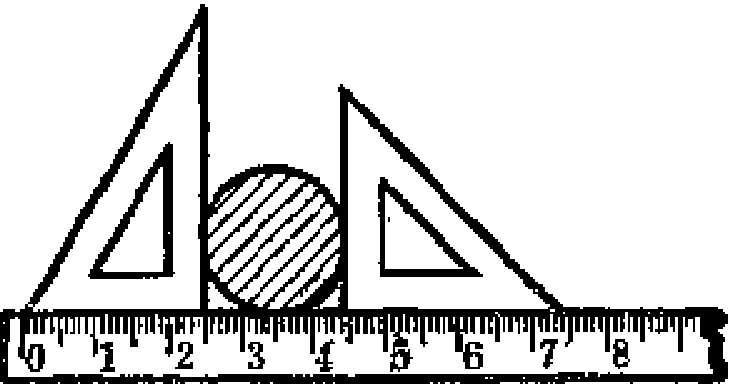
\includegraphics[width=8cm]{../pic/czjh2-ch7-xiti25-02.png}
    \caption*{(第 2 题)}
\end{figure}

\xiaoti{已知:如图, $\triangle ABC$ 内接于 $\yuan\,O$, $\angle CAE = \angle B$。如果
    (1) $AB$ 是直径; (2)$AB$ 为非直径的弦,
    求证: $AE$ 与 $\yuan\,O$ 相切于点 $A$。
}

\begin{figure}[htbp]
    \centering
    \begin{minipage}[b]{9cm}
        \centering
        \begin{minipage}[b]{4.4cm}
            \begin{tikzpicture}
    \tkzDefPoints{0/0/O}
    \tkzDefPoint(180:1.5){A}
    \tkzDefPoint(0:1.5){B}
    \tkzDefPoint(300:1.5){C}
    \tkzDefLine[perpendicular=through A,normed](O,A)  \tkzGetPoint{e}
    \tkzDefPointOnLine[pos=1.5](A,e)  \tkzGetPoint{E}

    \tkzDrawCircle[thick](O,A)
    \tkzDrawPoint(O)
    \tkzDrawPolygon(A,B,C)
    \tkzDrawLine[add=0 and 1](E,A)
    \tkzMarkAngle[size=.5](A,B,C)
    \tkzMarkAngle[size=.5](E,A,C)
    \tkzLabelPoints[below](O)
    \tkzLabelPoints[left](A)
    \tkzLabelPoints[right](B)
    \tkzLabelPoints[below](C)
    \tkzLabelPoints[left](E)
\end{tikzpicture}


        \end{minipage}
        \begin{minipage}[b]{4.4cm}
            \begin{tikzpicture}
    \tkzDefPoints{0/0/O}
    \tkzDefPoint(180:1.5){A}
    \tkzDefPoint(20:1.5){B}
    \tkzDefPoint(300:1.5){C}
    \tkzDefLine[perpendicular=through A,normed](O,A)  \tkzGetPoint{e}
    \tkzDefPointOnLine[pos=1.5](A,e)  \tkzGetPoint{E}

    \tkzDrawCircle[thick](O,A)
    \tkzDrawPoint(O)
    \tkzDrawPolygon(A,B,C)
    \tkzDrawLine[add=0 and 1](E,A)
    \tkzMarkAngle[size=.5](A,B,C)
    \tkzMarkAngle[size=.5](E,A,C)
    \tkzLabelPoints[below](O)
    \tkzLabelPoints[left](A)
    \tkzLabelPoints[right](B)
    \tkzLabelPoints[below](C)
    \tkzLabelPoints[left](E)
\end{tikzpicture}


        \end{minipage}
        \caption*{(第 3 题)}
    \end{minipage}
    \qquad
    \begin{minipage}[b]{5.6cm}
        \centering
        \begin{tikzpicture}
    \pgfmathsetmacro{\R}{1.8}
    \pgfmathsetmacro{\r}{1.4}

    \tkzDefPoints{0/0/O_2}
    \tkzDefPoint(180:\R){O_1}
    \tkzDefPoint(0:\R){C}
    \tkzInterCC[R](O_1,\r)(O_2,\R)  \tkzGetPoints{A}{B}

    \tkzDrawCircle[thick](O_1,A)
    \tkzDrawCircle[thick](O_2,A)
    \tkzDrawPoints(O_1, O_2)
    \tkzDrawSegments(O_1,C  A,C)

    \tkzLabelPoints[left](O_1)
    \tkzLabelPoints[below](O_2)
    \tkzLabelPoints[above=.2em](A)
    \tkzLabelPoints[below=.2em](B)
    \tkzLabelPoints[right](C)
\end{tikzpicture}


        \caption*{(第 4 题)}
    \end{minipage}
\end{figure}

\xiaoti{$\yuan\,O_2$ 经过 $\yuan\,O_1$ 的圆心, 与 $\yuan\,O_1$ 相交于 $A$、$B$ 两点。
    直线 $O_1O_2$ 交 $\yuan\,O_2$ 于点 $C$。
    求证: $AC$ 是 $\yuan\,O_1$ 的切线。
}

\xiaoti{两个同心圆中,大圆的弦 $AB$ 和 $AC$ 分别和小圆相切于点 $D$ 和 $E$。
    求证: $DE \pxqdy \exdfrac{1}{2} BC$。
}

\xiaoti{$MN$ 是 $\yuan\,O$ 的切线, $AB$ 是 $\yuan\,O$ 的直径。
    求证: 点 $A$ 、$B$ 与 $MN$ 的距离的和等于 $\yuan\,O$ 的直径。
}

\xiaoti{设 $AB$ 为 $\yuan\,O$ 的直径, $C$ 是 $\yuan\,O$ 上一点,
    $AD$ 和 $\yuan\,O$ 在点 $C$ 的切线相垂直,垂足为 $D$。
    求证: $AC$ 平分 $\angle DAB$。
}

\xiaoti{求证:以等腰三角形底边的中点为圆心,并且和一腰相切的圆,也和另一腰相切。}

\xiaoti{}%
\begin{xiaoxiaotis}%
    \xxt[\xxtsep]{作一个半径为 3 cm的圆,使它与已知直线 $l$ 相切于 $l$ 上一点 $A$;}

    \xxt{以直线 $l$ 外一点 $A$ 为圆心,作圆与直线 $l$ 相切。}

\end{xiaoxiaotis}

\xiaoti{已知:等腰梯形各边都与 $\yuan\,O$ 相切, $\yuan\,O$ 的直径为 6 cm,
    等腰梯形的腰等于 8 cm。 求梯形的面积。
}

\xiaoti{$PA$、$PB$ 是 $\yuan\,O$ 的切线, $A$、$B$ 是切点, 延长半径 $OB$ 到 $C$,
    使 $BC = OB$。 求证: $\angle APC = 3 \angle BPC$。
}

\xiaoti{$AB$、$CD$ 是 $\yuan\,O$ 的切线, $AB \pingxing CD$;
    $EF$ 也是 $\yuan\,O$ 的切线,它和 $AB$、$CD$ 分别相交于点 $E$ 和 $F$。
    求证: $\angle EOF = 90^\circ$。
}

\xiaoti{$PA$、$PB$ 为 $\yuan\,O$ 的切线, $AC$ 为经过切点 $A$ 的直径。
    求证: 切点 $B$ 和点 $C$ 的连线平行于 $PO$。
}

\xiaoti{过 $\yuan\,O$ 外的一点 $P$ 的直线 $PA$ 和 $PB$ 与 $\yuan\,O$ 相切于点 $A$ 和 $B$。
    $D$ 是 $\yuanhu{AB}$ 上任意一点, 过点 $D$ 的切线与 $PA$ 和 $PB$ 分别相交于点 $E$ 和 $F$。
    已知 $\angle P = \alpha$, 用 $\alpha$ 表示 $\angle EOF$。
}


\xiaoti{求证:}
\begin{xiaoxiaotis}

    \xxt{等边三角形的内心也是它的外心;}

    \xxt{等边三角形的外接圆半径 $R$ 是内切圆半径 $r$ 的 2 倍。}

\end{xiaoxiaotis}

\xiaoti{$\triangle ABC$ 中,内切圆 $I$ 和边 $BC$、$CA$、$AB$ 分别相切于点 $D$、$E$、$F$。
    求证: $\angle FDE = 90^\circ - \exdfrac{1}{2} \angle A$。
}

\xiaoti{$\triangle ABC$ 中, $E$ 是内心, $\angle A$ 的平分线和 $\triangle ABC$
    的外接圆相交于点 D。 求证: $DE = DB = DC$。
}

\xiaoti{圆外切四边形的周长为 48 厘米, 相邻的三条边的比为 $5:4:7$, 求四边形各边的长。}

\xiaoti{$ABCDEF$ 是 $\yuan\,O$ 的外切六边形。求证:
    $$ AB + CD + EF = BC + DE + FA \juhao $$
}

\xiaoti{已知: $\triangle ABC$ 的 $\angle A$ 的平分线和外接圆 $O$ 相交于点 $D$,
    $BE$ 是 $\yuan\,O$ 的切线。 求证: 点 $D$ 到 $BC$ 和到 $BE$ 的距离相等。
}

\xiaoti{$\yuan\,O$ 的弦 $AB$ 的延长线和切线 $EP$ 相交于点 $P$, $E$ 为切点。
    $\angle APE$ 的平分线和 $AE$、$BE$ 分別相交于点 $C$、$D$。
    求证: $\triangle CDE$ 是等腰三角形。
}

\xiaoti{已知: $PA$、$PB$ 与 $\yuan\,O$ 相切于点 $A$、$B$, $AC$ 是 $\yuan\,O$ 的直径。
    求证: $\angle APB = 2 \angle BAC$。
}

\begin{figure}[htbp]
    \centering
    \begin{minipage}[b]{7cm}
        \centering
        \begin{tikzpicture}
    \tkzDefPoints{0/0/O, 3.5/0.5/P}
    \tkzDefPoint(0:1.5){T}

    \tkzDefMidPoint(O,P)  \tkzGetPoint{Q}
    \tkzInterCC(O,T)(Q,P)  \tkzGetPoints{A}{B}
    \tkzDefPointOnLine[pos=2](A,O)  \tkzGetPoint{C}

    \tkzDrawCircle[thick](O,A)
    \tkzDrawPoint(O)
    \tkzDrawSegments(A,C  A,B  P,A  P,B)
    \tkzLabelPoints[left](O)
    \tkzLabelPoints[right](P)
    \tkzLabelPoints[above](A)
    \tkzLabelPoints[below](B)
    \tkzLabelPoints[below](C)
\end{tikzpicture}


        \caption*{(第 22 题)}
    \end{minipage}
    \qquad
    \begin{minipage}[b]{7cm}
        \centering
        \begin{tikzpicture}
    \pgfmathsetmacro{\R}{1.8}
    \pgfmathsetmacro{\r}{1.3}

    \tkzDefPoints{0/0/O}
    \tkzDefPoint(100:\R){A}
    \tkzDefPoint(20:\R){B}
    \tkzDefPoint(210:\r){Y}
    \tkzDefPoint(250:\r){Q}
    \tkzInterLC[common=Y](A,Y)(O,Y)  \tkzGetFirstPoint{X}
    \tkzInterLC[common=Q](B,Q)(O,Y)  \tkzGetFirstPoint{P}

    \tkzDrawCircle[thick](O,A)
    \tkzDrawCircle[thick](O,Y)
    \tkzDrawPoint(O)
    \tkzDrawSegments(A,Y  B,Q)

    \tkzLabelPoints[right](O)
    \tkzLabelPoints[above](A)
    \tkzLabelPoints[right](B)
    \tkzLabelPoints[right, yshift=-.3em](P)
    \tkzLabelPoints[below](Q)
    \tkzLabelPoints[above, xshift=-.2em](X)
    \tkzLabelPoints[below, xshift=-.3em](Y)
\end{tikzpicture}


        \caption*{(第 24 题)}
    \end{minipage}
\end{figure}

\xiaoti{圆内相交两弦中,一弦被交点所内分成的两条线段的长为 4 厘米、7 厘米,
    另一弦全长为 11.5 厘米。 求这弦被分成的两条线段的长。
}

\xiaoti{两个同心圆中, $A$、$B$ 为大圆上的任意两点, 过 $A$、$B$ 作小圆的的割线
    $AXY$ 和 $BPQ$。求证: $AX \cdot AY = BP \cdot BQ$。
}

\xiaoti{作一个正方形,使它的面积等于已知矩形的面积。}

\xiaoti{设 $C$ 为线段 $AB$ 的中点, $BCDE$ 是以 $BC$ 为边的正方形。
    以 $B$ 为圆心, $BD$ 为半径的圆与 $AB$ 及其延长线相交于点 $H$ 及 $K$。求证:
}
\begin{xiaoxiaotis}

    \xxt{$HC \cdot CK = AC^2$;}

    \xxt{$AH \cdot AK = 2 AC^2$。}

\end{xiaoxiaotis}

\end{enhancedline}
\end{xiaotis}



\section{圆和圆的位置关系}
\subsection{圆和圆的位置关系}\label{subsec:czjh2-7-13}

从图 \ref{fig:czjh2-7-49} 的一些圆形部件之间的相互位置关系中可以看出,同一平面内的两个圆,可能有下面的几种位置关系:

\begin{figure}[htbp]
    \centering
    \begin{minipage}[b]{8cm}
        \centering
        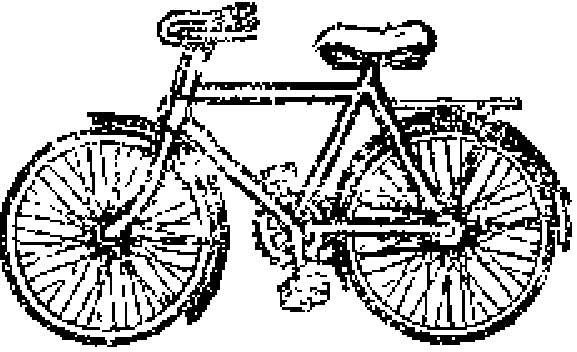
\includegraphics[width=7cm]{../pic/czjh2-ch7-49-1.png}
        \caption*{自行车}
    \end{minipage}
    \begin{minipage}[b]{6cm}
        \centering
        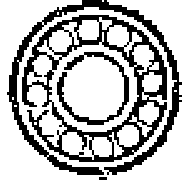
\includegraphics[width=3cm]{../pic/czjh2-ch7-49-2.png}
        \caption*{滚珠轴承}
    \end{minipage}
    \caption{}\label{fig:czjh2-7-49}
\end{figure}

(1) 两个圆没有公共点,并且每个圆上的点都在另一个圆的外部时,叫做这两个圆\zhongdian{外离}(图 \ref{fig:czjh2-7-50} 甲)。

(2) 两个圆有唯一的公共点,并且除了这个公共点以外,每个圆上的点都在另一个圆的外部时,
叫做这两个圆\zhongdian{外切}(图 \ref{fig:czjh2-7-50} 乙)。这个唯一的公共点叫做\zhongdian{切点}。


\begin{figure}[htbp]
    \centering
    \begin{minipage}[b]{4.7cm}
        \centering
        \begin{tikzpicture}[scale=.8] % 这组图中, O_1 固定不动, O_2 向 O_1 移近。所以以 O_1 为原点
    \pgfmathsetmacro{\R}{1.5}
    \pgfmathsetmacro{\r}{1.2}

    \tkzDefPoints{0/0/O_1, -3.1/0/O_2}
    \tkzDefPoint(60:\R){M}
    \tkzDefShiftPoint[O_2](60:\r){N}

    \tkzDrawCircle[thick](O_1,M)
    \tkzDrawCircle[thick](O_2,N)
    \tkzDrawSegments(O_1,M  O_2,N  O_1,O_2)
    \tkzLabelSegment[midway, left](O_1,M){$R$}
    \tkzLabelSegment[midway, left](O_2,N){$r$}
    \tkzLabelPoints[right](O_1)
    \tkzLabelPoints[left](O_2)
\end{tikzpicture}


        \caption*{甲}
    \end{minipage}
    \qquad
    \begin{minipage}[b]{4.5cm}
        \centering
        \begin{tikzpicture}[scale=.8]
    \pgfmathsetmacro{\R}{1.5}
    \pgfmathsetmacro{\r}{1.2}

    \tkzDefPoints{0/0/O_1, -2.7/0/O_2, -\R/0/T}
    \tkzDefPoint(60:\R){M}
    \tkzDefShiftPoint[O_2](60:\r){N}

    \tkzDrawCircle[thick](O_1,M)
    \tkzDrawCircle[thick](O_2,N)
    \tkzDrawSegments(O_1,M  O_2,N  O_1,O_2)
    \tkzLabelSegment[midway, left](O_1,M){$R$}
    \tkzLabelSegment[midway, left](O_2,N){$r$}
    \tkzLabelPoints[right](O_1)
    \tkzLabelPoints[left](O_2)
    \tkzLabelPoints[above=1.3em](T)
\end{tikzpicture}


        \caption*{乙}
    \end{minipage}
    \qquad
    \begin{minipage}[b]{4.5cm}
        \centering
        \begin{tikzpicture}[scale=.8]
    \pgfmathsetmacro{\R}{1.5}
    \pgfmathsetmacro{\r}{1.2}

    \tkzDefPoints{0/0/O_1, -2.3/0/O_2}
    \tkzDefPoint(60:\R){M}
    \tkzDefShiftPoint[O_2](60:\r){N}
    \tkzInterCC(O_1,M)(O_2,N)  \tkzGetPoints{B}{A}

    \tkzDrawCircle[thick](O_1,M)
    \tkzDrawCircle[thick](O_2,N)
    \tkzDrawSegments(O_1,M  O_2,N  O_1,O_2)
    \tkzLabelSegment[midway, left](O_1,M){$R$}
    \tkzLabelSegment[midway, left](O_2,N){$r$}
    \tkzLabelPoints[right](O_1)
    \tkzLabelPoints[left](O_2)
    \tkzLabelPoints[above=.5em](A)
    \tkzLabelPoints[below=.5em](B)
\end{tikzpicture}


        \caption*{丙}
    \end{minipage}
    \qquad
    \begin{minipage}[b]{4.5cm}
        \centering
        \begin{tikzpicture}[scale=.8]
    \pgfmathsetmacro{\R}{1.5}
    \pgfmathsetmacro{\r}{1.2}

    \tkzDefPoints{0/0/O_1, \r-\R/0/O_2, -\R/0/T}
    \tkzDefPoint(60:\R){M}
    \tkzDefShiftPoint[O_2](60:\r){N}

    \tkzDrawCircle[thick](O_1,M)
    \tkzDrawCircle[thick](O_2,N)
    \tkzDrawSegments(O_1,M  O_2,N  O_1,T)
    \tkzLabelSegment[pos=.7, right](O_1,M){$R$}
    \tkzLabelSegment[midway, left](O_2,N){$r$}
    \tkzLabelPoints[right](O_1)
    \tkzLabelPoints[below](O_2)
    \tkzLabelPoints[left](T)
\end{tikzpicture}


        \caption*{丁}
    \end{minipage}
    \qquad
    \begin{minipage}[b]{7cm}
        \centering
        \begin{minipage}[b]{2.8cm}
            \begin{tikzpicture}[scale=.8]
    \pgfmathsetmacro{\R}{1.5}
    \pgfmathsetmacro{\r}{1.2}

    \tkzDefPoints{0/0/O_1, \r-\R+.15/0/O_2, -\R/0/T}
    \tkzDefPoint(60:\R){M}
    \tkzDefShiftPoint[O_2](60:\r){N}

    \tkzDrawCircle[thick](O_1,M)
    \tkzDrawCircle[thick](O_2,N)
    \tkzDrawSegments(O_1,M  O_2,N  O_1,T)
    \tkzLabelSegment[pos=.4, right](O_1,M){$R$}
    \tkzLabelSegment[midway, left](O_2,N){$r$}
    \tkzLabelPoints[right](O_1)
    \tkzLabelPoints[below](O_2)
\end{tikzpicture}


        \end{minipage}
        \begin{minipage}[b]{2.8cm}
            \begin{tikzpicture}[scale=.8]
    \pgfmathsetmacro{\R}{1.5}
    \pgfmathsetmacro{\r}{1.2}

    \tkzDefPoints{0/0/O_1, 0/0/O_2} % O_1 = O_2
    \tkzDefPoint(15:\R){M}
    \tkzDefShiftPoint[O_2](60:\r){N}

    \tkzDrawCircle[thick](O_1,M)
    \tkzDrawCircle[thick](O_2,N)
    \tkzDrawSegments(O_1,M  O_2,N)
    \tkzLabelSegment[midway, below](O_1,M){$R$}
    \tkzLabelSegment[midway, left](O_2,N){$r$}
    \tkzLabelPoint[left](O_1){$O$}
\end{tikzpicture}


        \end{minipage}
        \caption*{戊}
    \end{minipage}
    \caption{}\label{fig:czjh2-7-50}
\end{figure}

(3) 两个圆有两个公共点时,叫做这两个圆\zhongdian{相交}(图 \ref{fig:czjh2-7-50} 丙)。

(4) 两个圆有唯一的公共点,并且除了这个公共点以外,一个圆上的点都在另一个圆的内部时,
叫做这两个圆\zhongdian{内切}(图 \ref{fig:czjh2-7-50} 丁)。这个唯一的公共点叫做\zhongdian{切点}。

(5) 两个圆没有公共点,并且一个圆上的点都在另一个圆的内部时,叫做这两个圆\zhongdian{内含}(图 \ref{fig:czjh2-7-50} 戊)。
两圆同心是两圆内含的一种特例。

从图 \ref{fig:czjh2-7-50} 可以看出,圆和圆的位置关系与两圆半径、圆心距的大小有关。
如果两圆的半径分别为 $R$ 和 $r$, 圆心距为 $d$,那么


\zhongdian{(1) $\bm{d > R + r} \dengjiayu$ 两圆外离;}

\zhongdian{(2) $\bm{d = R + r} \dengjiayu$ 两圆外切;}

\zhongdian{(3) $\bm{R - r < d < R + r \; (R \geqslant r)} \dengjiayu$ 两圆相交;}

\zhongdian{(4) $\bm{d = R - r \; (R > r)} \dengjiayu$ 两圆内切;}

\zhongdian{(5) $\bm{d < R - r \; (R > r)} \dengjiayu$ 两圆内含。}

在图 \ref{fig:czjh2-7-50} 中,设想 $\yuan\,O_1$ 固定不动, $\yuan\,O_2$ 从一方移近并进入 $\yuan\,O_1$,
直到圆心 $O_2$ 和 $O_1$ 重合,就可以看到上面所说的各种情况。

关于相交的两圆,有下面的定理:

\begin{dingli}[定理]
    相交两圆的连心线(经过两个圆心的直线),垂直平分两圆的公共弦。
\end{dingli}

已知:$\yuan\,O_1$ 和 $\yuan\,O_1$ 相交于点 $A$ 和 $B$ (图 \ref{fig:czjh2-7-51})。

求证: 直线 $O_1O_2$ 垂直平分线段 $AB$。

\zhengming 因为,经过圆心 $O_1$ 和 $O_2$ 的直线是 $\yuan\,O_1$ 的对称轴,又是 $\yuan\,O_2$ 的对称轴,
所以, $\yuan\,O_1$ 和 $\yuan\,O_2$ 的公共点 $A$ 的对称点在 $\yuan\,O_1$ 上,又在 $\yuan\,O_1$ 上。
这个对称点只能是两圆的另一个交点 $B$。 这样,连心线 $O_1O_2$ 就是连结对称点 $A$、$B$ 的线段的垂直平分线。

\begin{figure}[htbp]
    \centering
    \begin{minipage}[b]{5.2cm}
        \centering
        \begin{tikzpicture}[scale=.9]
    \pgfmathsetmacro{\R}{1.5}
    \pgfmathsetmacro{\r}{1.2}

    \tkzDefPoints{0/0/O_1, 2.2/0/O_2}
    \tkzDefPoint(60:\R){M}
    \tkzDefShiftPoint[O_2](60:\r){N}
    \tkzInterCC(O_1,M)(O_2,N)  \tkzGetPoints{A}{B}

    \tkzDrawCircle[thick](O_1,M)
    \tkzDrawCircle[thick](O_2,N)
    \tkzDrawPoints(O_1, O_2)
    \tkzDrawLine[add=.8 and .8](O_1,O_2)
    \tkzDrawSegments(A,B)
    \tkzLabelPoints[below](O_1)
    \tkzLabelPoints[below](O_2)
    \tkzLabelPoints[above=.5em](A)
    \tkzLabelPoints[below=.5em](B)
\end{tikzpicture}


        \caption*{} % 与下面的图水平对齐
        \caption{}\label{fig:czjh2-7-51}
    \end{minipage}
    \qquad
    \begin{minipage}[b]{10.5cm}
        \centering
        \begin{minipage}[b]{5.6cm}
            \centering
            \begin{tikzpicture}[scale=.9]
    \pgfmathsetmacro{\R}{1.5}
    \pgfmathsetmacro{\r}{1.0}

    \tkzDefPoints{0/0/O_1, \R+\r/0/O_2, \R/0/T}
    \tkzDefPoint(60:\R){M}
    \tkzDefShiftPoint[O_2](60:\r){N}

    \tkzDrawCircle[thick](O_1,M)
    \tkzDrawCircle[thick](O_2,N)
    \tkzDrawPoints(O_1, O_2)
    \tkzDrawLine[add=.7 and .5](O_1,O_2)
    \tkzLabelPoints[below](O_1)
    \tkzLabelPoints[below](O_2)
    \tkzLabelPoints[left, yshift=.5em](T)
\end{tikzpicture}


            \caption*{甲}
        \end{minipage}
        \begin{minipage}[b]{4cm}
            \centering
            \begin{tikzpicture}[scale=.9]
    \pgfmathsetmacro{\R}{1.5}
    \pgfmathsetmacro{\r}{1.0}

    \tkzDefPoints{0/0/O_1, \r-\R/0/O_2, -\R/0/T}
    \tkzDefPoint(60:\R){M}
    \tkzDefShiftPoint[O_2](60:\r){N}

    \tkzDrawCircle[thick](O_1,M)
    \tkzDrawCircle[thick](O_2,N)
    \tkzDrawPoints(O_1, O_2)
    \tkzDrawLine[add=3.5 and 3](O_1,O_2)
    \tkzLabelPoints[below, xshift=.2em](O_1)
    \tkzLabelPoints[below, xshift=-.2em](O_2)
    \tkzLabelPoints[left, yshift=.5em](T)
\end{tikzpicture}


            \caption*{乙}
        \end{minipage}
        \caption{}\label{fig:czjh2-7-52}
    \end{minipage}
\end{figure}


关于相切的两圆,有下面的定理:

\begin{dingli}[定理]
    相切两圆的连心线,经过切点。
\end{dingli}

已知: $\yuan\,O_1$ 和 $\yuan\,O_2$ 相切于点 $T$(图 \ref{fig:czjh2-7-52})。

求证: 连心线 $O_1O_2$ 经过切点 $T$。

\zhengming 用反证法。

假设 $O_1O_2$ 不经过 $\yuan\,O_1$ 和 $\yuan\,O_2$ 的切点 $T$ (即点 $T$ 不在 $O_1O_2$ 上),
那么,点 $T$ 关于 $O_1O_2$ 的对称点 $T'$ 也不在 $O_1O_2$ 上。
由于直线 $O_1O_2$ 是 $\yuan\,O_1$ 的对称轴,又是 $\yuan\,O_2$ 的对称轴,
并且点 $T$ 是 $\yuan\,O_1$ 和 $\yuan\,O_2$ 的公共点,
所以点 $T$ 的对称点 $T'$ 也是 $\yuan\,O_1$ 和 $\yuan\,O_1$ 的公共点。
这和题设 $\yuan\,O_1$ 和 $\yuan\,O_2$ 相切相矛盾,因此假设不能成立。
连心线 $O_1O_2$ 经过切点 $T$。


\liti[0] 已知:两个等圆 $\yuan\,O_1$ 和 $\yuan\,O_2$ 相交于 $A$、$B$ 两点,
$\yuan\,O_1$ 经过点 $O_2$(图 \ref{fig:czjh2-7-53})。求 $\angle O_1AB$ 的度数。

\jie $\because$ \quad $\yuan\,O_1$ 经过点 $O_2$, $\yuan\,O_1$、$\yuan\,O_2$ 是等圆,

$\therefore$ \quad $O_1A = O_1O_2 = O_2A$。

$\therefore$ \quad $\angle O_1AO_2 = 60^\circ$。

又 $\because$ \quad $AB \perp O_1O_2$,

$\therefore$ \quad $\angle O_1AB = 30^\circ$。


\begin{figure}[htbp]
    \centering
    \begin{minipage}[b]{5.2cm}
        \centering
        \begin{tikzpicture}[scale=.9]
    \pgfmathsetmacro{\R}{1.5}

    \tkzDefPoints{0/0/O_1, \R/0/O_2}
    \tkzInterCC[R](O_1,\R)(O_2,\R)  \tkzGetPoints{A}{B}

    \tkzDrawCircle[thick](O_1,A)
    \tkzDrawCircle[thick](O_2,A)
    \tkzDrawPoints(O_1, O_2)
    \tkzDrawSegments(O_1,O_2  A,B  O_1,A  O_2,A)
    \tkzLabelPoints[left](O_1)
    \tkzLabelPoints[right](O_2)
    \tkzLabelPoints[above=.2em](A)
    \tkzLabelPoints[below=.2em](B)
\end{tikzpicture}


        \caption{}\label{fig:czjh2-7-53}
    \end{minipage}
    \qquad
    \begin{minipage}[b]{10.5cm}
        \centering
        \begin{minipage}[b]{5.6cm}
            \centering
            \begin{tikzpicture}[scale=.9]
    \pgfmathsetmacro{\R}{1.5}
    \pgfmathsetmacro{\r}{1.0}

    \tkzDefPoints{0/0/O_1, \R+\r/0/O_2, \r/0/T}
    \tkzDefPoint(120:\r){A}
    \tkzInterLC[common=T](A,T)(O_2,T)  \tkzGetFirstPoint{B}

    \tkzDrawCircle[thick](O_1,T)
    \tkzDrawCircle[thick](O_2,T)
    \tkzDrawPoints(O_1, O_2)
    \tkzDrawSegments(O_1,A  O_2,B  A,B)
    \tkzLabelPoints[below](O_1)
    \tkzLabelPoints[right](O_2)
    \tkzLabelPoints[above](A)
    \tkzLabelPoints[below](B)
    \tkzLabelPoints[right, yshift=.5em](T)
\end{tikzpicture}


        \end{minipage}
        \begin{minipage}[b]{4cm}
            \centering
            \begin{tikzpicture}[scale=.9]
    \pgfmathsetmacro{\R}{1.5}
    \pgfmathsetmacro{\r}{1.0}

    \tkzDefPoints{0/0/O_1, \R-\r/0/O_2, -\r/0/T}
    \tkzDefPoint(60:\r){A}
    \tkzInterLC[common=T](A,T)(O_2,T)  \tkzGetFirstPoint{B}

    \tkzDrawCircle[thick](O_1,T)
    \tkzDrawCircle[thick](O_2,T)
    \tkzDrawPoints(O_1, O_2)
    \tkzDrawSegments(O_1,A  O_2,B  T,B)
    \tkzLabelPoints[below, xshift=-.5em](O_1)
    \tkzLabelPoints[below](O_2)
    \tkzLabelPoints[above, xshift=-.2em](A)
    \tkzLabelPoints[above right](B)
    \tkzLabelPoints[left](T)
\end{tikzpicture}


        \end{minipage}
        \caption*{(第 4 题)}
    \end{minipage}
\end{figure}



\begin{lianxi}

\xiaoti{$\yuan\,O_1$ 和 $\yuan\,O_2$ 的半径分别为 3 厘米和 4 厘米,设}
\begin{xiaoxiaotis}

    \begin{tblr}{columns={12em, colsep=0pt}}
        \xxt{$O_1O_2 = 8$ 厘米;} & \xxt{$O_1O_2 =   7$ 厘米;} & \xxt{$O_1O_2 = 5$ 厘米;} \\
        \xxt{$O_1O_2 = 1$ 厘米;} & \xxt{$O_1O_2 = 0.5$ 厘米;} & \xxt{$O_1$ 和 $O_2$ 重合。}
    \end{tblr}

    \quad $\yuan\,O_1$ 和 $\yuan\,O_2$ 的位置关系怎样?
\end{xiaoxiaotis}


\xiaoti{三角形的三边长分别力 4 厘米、5 厘米、6厘米,以各顶点为圆心的三个圆两两外切。
    求各圆的半径。如果三边长分别为 $a$、$b$、$c$ 呢?
}

\xiaoti{已知: $\yuan\,O_1$ 和 $\yuan\,O_2$ 相交于点 $C$ 和 $D$, $O_2O_1$ 的延长线和 $\yuan\,O_1$ 相交于点 $A$,
    $AC$、$AD$ 分别和 $\yuan\,O_2$ 相交于点 $E$、$F$。 求证: $CE = DF$。
}

\xiaoti{已知:$\yuan\,O_1$ 和 $\yuan\,O_2$ 相切于点 $T$, 经过切点 $T$ 的直线与 $\yuan\,O_1$ 和 $\yuan\,O_2$
    分别相交于另一点 $A$ 和 $B$。求证: $O_1A \pingxing O_2B$。
}

\end{lianxi}


\subsection{两圆的公切线}\label{subsec:czjh2-7-14}

很多机器上的传动带与主动轮、从动轮之间的位置关系,
给我们以一条直线和两个圆同时相切的形象(图 \ref{fig:czjh2-7-54})。

和两个圆都相切的直线,叫做\zhongdian{两圆的公切线}。
两个圆在公切线同旁时,这样的公切线叫做\zhongdian{外公切线}(如图 \ref{fig:czjh2-7-54} 甲)。
两个圆在公切线两旁时,这样的公切线叫做\zhongdian{内公切线}(如图 \ref{fig:czjh2-7-54} 乙)。
公切线上的两个切点的距离叫做\zhongdian{公切线的长}。

\begin{figure}[htbp]
    \centering
    \begin{minipage}[b]{7cm}
        \centering
        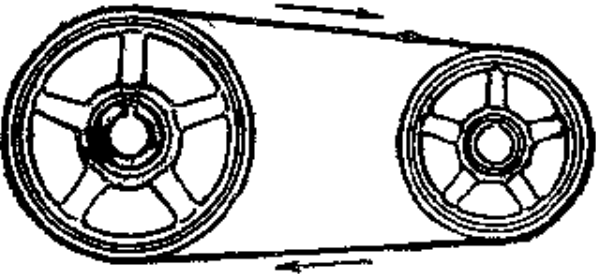
\includegraphics[width=5.5cm]{../pic/czjh2-ch7-54-a.png}
        \caption*{甲}
    \end{minipage}
    \qquad
    \begin{minipage}[b]{7cm}
        \centering
        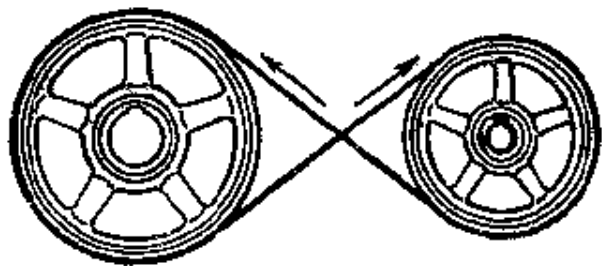
\includegraphics[width=5.5cm]{../pic/czjh2-ch7-54-b.png}
        \caption*{乙}
    \end{minipage}
    \caption{}\label{fig:czjh2-7-54}
\end{figure}



下面我们说明两圆公切线的作法。

两圆外离、外切或相交时,外公切线的作法如下。

已知: $\yuan\,O_1$ 和 $\yuan\,O_2$ 的半径分别为 $R$ 和 $r$($R > r$),
$O_1O_2 > R - r$ (图 \ref{fig:czjh2-7-55})。

求作: $\yuan\,O_1$ 和 $\yuan\,O_2$ 的外公切线。

分析:前面已经学过经过一点作一个圆的切线,这启发我们想办法把作两个圆的公切线的问题,
化为过一个点作一个圆的切线的问题来解决。
假设把 $\yuan\,O_1$ 和 $\yuan\,O_2$ 的半径同时缩短 $r$,
那么 $\yuan\,O_1$ 变为与它同心,半径是 $R-r$ 的圆,而 $\yuan\,O_2$ 变为一个点 $O_2$。
因为过点 $O_2$ 能够作直线与半径为 $R-r$ 的圆相切,那么只要把切线平行移动 $r$,
就可以得到 $\yuan\,O_1$ 和 $\yuan\,O_2$ 的公切线(图 \ref{fig:czjh2-7-55})。

\zuofa 1. 以 $O_1$ 为圆心, $R-r$ 为半径作圆, 从 $O_2$ 作过个圆的切线 $O_2E$, $E$ 为切点。

2. 连结 $O_1E$, 并延长交 $\yuan\,O_1$ 于点 $A$。

3. 经过圆心 $O_2$ 作 $O_2B \pingxing O_1A$, 并交 $\yuan\,O_2$ 于点 $B$。

4. 作直线 $AB$。

$AB$ 就是所求的一条公切线。

\zhengming 由作法, $O_2E \perp O_1A$, $O_2B \pingxing O_1A$,
$EA = O_1A - O_1E = R - (R-r) = r = O_2B$,
所以,四边形 $EO_2BA$ 是矩形。于是, $O_1A \perp AB$, $O_2B \perp AB$。
因此,$AB$ 是 $\yuan\,O_1$ 的切线, 又是 $\yuan\,O_2$ 的切线,
即 $AB$ 是 $\yuan\,O_1$ 和 $\yuan\,O_2$ 的外公切线。

由作法,还可以知道,从 $O_2$ 向以 $O_1$ 为圆心, $R-r$ 为半径的圆,
可以作出两条切线( $O_2E$ 和 $O_2F$),因此,可以作出 $\yuan\,O_1$ 和
$\yuan\,O_1$ 的两条外公切线($AB$ 和 $CD$)。

\begin{figure}[htbp]
    \centering
    \begin{minipage}[b]{7cm}
        \centering
        \begin{tikzpicture}
    \pgfmathsetmacro{\R}{1.5}
    \pgfmathsetmacro{\r}{0.7}

    \tkzDefPoints{0/0/O_1, 4/0/O_2}
    \tkzDefPoint(0:\R){M}
    \tkzDefShiftPoint[O_2](0:\r){N}
    \tkzDrawCircle[very thick](O_1,M)
    \tkzDrawCircle[very thick](O_2,N)
    \tkzDrawSegment[dashed](O_1,O_2)
    \tkzLabelPoints[left](O_1)
    \tkzLabelPoints[right](O_2)

    % 1
    \tkzDefPoint(0:\R-\r){T1}
    \tkzDrawCircle(O_1,T1)
    \tkzDefMidPoint(O_1,O_2)  \tkzGetPoint{T2}
    \tkzInterCC(O_1,T1)(T2,O_1)  \tkzGetPoints{E}{F}
    \tkzDrawSegment(O_2,E)
    \tkzLabelPoints[above left](E)

    % 2
    \tkzInterLC(O_1,E)(O_1,M)  \tkzGetSecondPoint{A}
    \tkzDrawSegment(O_1,A)
    \tkzLabelPoints[above](A)

    % 3
    \tkzDefLine[parallel=through O_2](O_1,A)  \tkzGetPoint{b}
    \tkzInterLC(O_2,b)(O_2,N)  \tkzGetSecondPoint{B}
    \tkzDrawSegment(O_2,B)
    \tkzLabelPoints[above](B)

    % 4
    \tkzDrawLine[very thick, add=0.3 and 0.2](A,B)

    % ex-1
    \tkzDrawSegment[dashed](O_2,F)
    \tkzLabelPoints[below left](F)

    % ex-2
    \tkzInterLC(O_1,F)(O_1,M)  \tkzGetSecondPoint{C}
    \tkzDrawSegment[dashed](O_1,C)
    \tkzLabelPoints[below](C)

    % ex-3
    \tkzDefLine[parallel=through O_2](O_1,C)  \tkzGetPoint{d}
    \tkzInterLC(O_2,d)(O_2,N)  \tkzGetSecondPoint{D}
    \tkzDrawSegment[dashed](O_2,D)
    \tkzLabelPoints[below](D)

    % ex-4
    \tkzDrawLine[very thick, add=0.3 and 0.2](C,D)

    % 标注半径
    \tkzLabelSegment[pos=.5, right](O_1,C){$R$}
    \tkzLabelSegment[pos=.5, left](O_2,B){$r$}

    \tkzDefMidPoint(O_1,E)  \tkzGetPoint{X1}
    \tkzDefPoint(150:\R-\r){X2}
    \tkzDrawSegment[-latex](X2,X1)
    \tkzLabelSegment[pos=.05, left](X2,X1){$R-r$}
\end{tikzpicture}


        \caption{}\label{fig:czjh2-7-55}
    \end{minipage}
    \qquad
    \begin{minipage}[b]{7.2cm}
        \centering
        \begin{tikzpicture}
    \pgfmathsetmacro{\R}{1.5}
    \pgfmathsetmacro{\r}{0.7}

    \tkzDefPoints{0/0/O_1, 4/0/O_2}
    \tkzDefPoint(210:\R){M}
    \tkzDefShiftPoint[O_2](50:\r){N}
    \tkzDrawCircle[very thick](O_1,M)
    \tkzDrawCircle[very thick](O_2,N)
    \tkzDrawSegment[dashed](O_1,O_2)
    \tkzLabelPoints[below=.3em](O_1)
    \tkzLabelPoints[below=.2em, xshift=.2em](O_2)

    % 1 以 O_1 为圆心,R+r 为半径作圆,O_2E 为切线
    \tkzDefPoint(0:\R+\r){T1}
    \tkzDrawCircle(O_1,T1)
    \tkzDefMidPoint(O_1,O_2)  \tkzGetPoint{T2}
    \tkzInterCC(O_1,T1)(T2,O_1)  \tkzGetPoints{E}{F}
    \tkzDrawLine[add=0.3 and 0.3](O_2,E)
    \tkzLabelPoints[above right](E)

    % 2
    \tkzInterLC(O_1,E)(O_1,M)  \tkzGetSecondPoint{A}
    \tkzDrawSegment(O_1,E)
    \tkzLabelPoints[above=.2em](A)

    % 3 O_2B 平行于 O_1A
    \tkzDefLine[parallel=through O_2](O_1,A)  \tkzGetPoint{b}
    \tkzInterLC(O_2,b)(O_2,N)  \tkzGetFirstPoint{B}
    \tkzDrawSegment(O_2,B)
    \tkzLabelPoints[below](B)

    % 4
    \tkzDrawLine[very thick, add=0.3 and 0.2](A,B)

    % ex-1
    \tkzDrawLine[dashed, add=0.3 and 0.3](O_2,F)
    \tkzLabelPoints[below=.2em, xshift=-.2em](F)

    % ex-2
    \tkzInterLC(O_1,F)(O_1,M)  \tkzGetSecondPoint{C}
    \tkzDrawLine[dashed, add=0 and 0.2](O_1,F)
    \tkzLabelPoints[below=.2em, xshift=-.2em](C)

    % ex-3
    \tkzDefLine[parallel=through O_2](O_1,C)  \tkzGetPoint{d}
    \tkzInterLC(O_2,d)(O_2,N)  \tkzGetSecondPoint{D}
    \tkzDrawSegment[dashed](O_2,D)
    \tkzLabelPoints[above](D)

    % ex-4
    \tkzDrawLine[very thick, add=0.3 and 0.2](C,D)

    % 标注半径
    \tkzDrawSegment[thick](O_1,M)
    \tkzLabelSegment[pos=.5, left, yshift=.3em](O_1,M){$R$}
    \tkzDrawSegment[thick](O_2,N)
    \tkzLabelSegment[pos=.6, left](O_2,N){$r$}
\end{tikzpicture}


        \caption{}\label{fig:czjh2-7-56}
    \end{minipage}
\end{figure}

仿照上面的分析,可以得出两圆外离($O_1O_2 > R+r$)时的内公切线的作法(图 \ref{fig:czjh2-7-56})。

两圆外切(或内切)时,经过切点作直线垂直于它们的连心线,就得到它们的内公切线(或外公切线)。

从公切线的作法可知,如果两个圆有两条外公切线或内公切线,那么它们的长相等。

\begin{dingli}[定理]
    两圆的两条外公切线的长相等;
    两圆的两条内公切线的长也相等。
\end{dingli}


\begin{wrapfigure}[8]{r}{6cm}
    \centering
    \begin{tikzpicture}
    \pgfmathsetmacro{\R}{1.5}
    \pgfmathsetmacro{\r}{1.0}

    \tkzDefPoints{0/0/O_1, \R/0/A, \R+\r/0/O_2}
    \tkzDrawCircle[very thick](O_1,A)
    \tkzDrawCircle[very thick](O_2,A)
    \tkzDrawPoints(O_1, O_2)
    \tkzLabelPoints[right](O_1, O_2)
    \tkzLabelPoints[left](A)

    % 绘制外公切线 BC
    \tkzDefSimilitudeCenter[ext](O_1,A)(O_2,A)  \tkzGetPoint{J}
    \tkzDefLine[tangent from = J](O_1,A)  \tkzGetSecondPoint{B}
    \tkzDefLine[tangent from = J](O_2,A)  \tkzGetSecondPoint{C}
    \tkzDrawLine[very thick, add=0.5 and 0.4](B,C)
    \tkzLabelPoints[above](B,C)

    %
    \tkzDrawSegments[very thick](A,B  A,C)

    % 辅助线
    \tkzDefShiftPoint[A](0,1){a}
    \tkzInterLL(A,a)(B,C)  \tkzGetPoint{O}
    \tkzDrawLine[dashed, add=1.5 and 0.5](A,O)
    \tkzLabelPoints[right, yshift=.5em](O)
\end{tikzpicture}


    \caption{}\label{fig:czjh2-7-57}
\end{wrapfigure}

\liti[0] 如图 \ref{fig:czjh2-7-57}, $\yuan\,O_1$ 和 $\yuan\,O_2$ 外切于点 $A$,
$BC$ 是 $\yuan\,O_1$ 和 $\yuan\,O_2$ 的公切线, $B$、$C$ 为切点。

求证: $AB \perp AC$。

\zhengming 过点 $A$ 作 $\yuan\,O_1$ 和 $\yuan\,O_2$ 的内公切线交 $BC$ 于点 $O$。

因为 $OB$、$OA$ 是 $\yuan\,O_1$ 的两条切线,

$\therefore$ \quad $OB = OA$。

同理 \quad $OC = OA$。

$\therefore$ \quad $OB = OA = OC$。

$\therefore$ \quad $AB \perp AC$。



\begin{lianxi}


\xiaoti{已知 $\yuan\,O_1$ 和 $\yuan\,O_2$ 的半径分别为 $R = 4$ 屋米, $r = 1.5$ 厘米,$O_1O_2 = 6.5$ 厘米。}
\begin{xiaoxiaotis}

    \xxt{作 $\yuan\,O_1$ 和 $\yuan\,O_2$ 的外公切线,量出外公切线的长(精确到 0.1 厘米)
        及外公切线与连心线所成的角度(精确到 $1^\circ$);
    }

    \xxt{计算出 (1) 中的长度和角度。}

\end{xiaoxiaotis}

\xiaoti{已知 $\yuan\,O_1$ 和 $\yuan\,O_2$ 的半径分别为 $R = 2.5$ 厘米, $r = 1.5$ 厘米,
    $O_1O_2 = 6$ 厘米, 作 $\yuan\,O_1$ 和 $\yuan\,O_2$ 的内公切线。
}

\end{lianxi}


\subsection{相切在作图中的应用}\label{subsec:czjh2-7-15}

运动场上的跑道和有些凸轮的轮廓线(图 \ref{fig:czjh2-7-58})等,是由线段和圆弧或几段圆弧平滑地连接起来的。

\begin{figure}[htbp]
    \centering
    \begin{minipage}[b]{6cm}
        \centering
        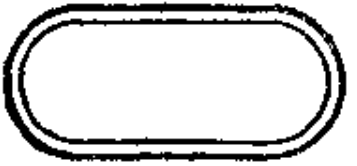
\includegraphics[width=5.5cm]{../pic/czjh2-ch7-58-1.png}
    \end{minipage}
    \qquad
    \begin{minipage}[b]{4cm}
        \centering
        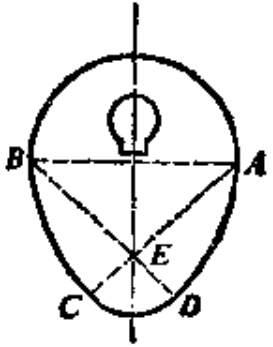
\includegraphics[width=3.5cm]{../pic/czjh2-ch7-58-2.png}
    \end{minipage}
    \caption{}\label{fig:czjh2-7-58}
\end{figure}

线段所在的直线(圆弧所在的圆)与圆弧所在的圆相切于某一点,并且在切点的两侧,
就说线段(圆弧)和圆弧在这一点\zhongdian{连接}。
如图 \ref{fig:czjh2-7-59} 中,线段 $AB$ 和弧 $\yuanhu{AC}$ 在点 $A$ 连接,
图 \ref{fig:czjh2-7-60} 中, $\yuanhu{AB}$ 和 $\yuanhu{AC}$ 在点 $A$ 连接。

\begin{figure}[htbp]
    \centering
    \begin{minipage}[b]{5cm}
        \centering
        \begin{tikzpicture}
    \pgfmathsetmacro{\R}{1.5}

    \tkzDefPoints{0/0/O}
    \tkzDefPoint(270:\R){A}
    \tkzDefShiftPoint[A](2,0){B}
    \tkzDefShiftPoint[A](-2,0){B'}
    \tkzDefPoint(140:\R){C}

    \tkzDrawPoint(O)
    \tkzDrawArc[dashed](O,A)(C)
    \tkzDrawArc[thick](O,C)(A)
    \tkzDrawSegment[red](O,C)
    \tkzLabelSegment[above](O,C){$R$}
    \tkzDrawSegment[dashed](O,A)
    \tkzLabelPoints[right](O)
    \tkzLabelPoints[left](C)

    \tkzDrawSegment[thick](A,B)
    \tkzDrawSegment[dashed](A,B')
    \tkzLabelSegment[pos=1, left](B,B'){$l$}
    \tkzLabelPoints[below](A)
    \tkzLabelPoints[right](B)
\end{tikzpicture}


        \caption*{} % 与下面的图水平对齐
        \caption{}\label{fig:czjh2-7-59}
    \end{minipage}
    \qquad
    \begin{minipage}[b]{10.5cm}
        \centering
        \begin{minipage}[b]{5.6cm}
            \centering
            \begin{tikzpicture}
    \pgfmathsetmacro{\R}{1.5}
    \pgfmathsetmacro{\r}{0.8}

    \tkzDefPoints{0/0/O_1, \R+\r/0/O_2, \R/0/A}
    \tkzDefPoint(70:\R){B}
    \tkzDefPoint(60:\R){M}
    \tkzDefShiftPoint[O_2](270:\r){C}
    \tkzDefShiftPoint[O_2](60:\r){N}
    \tkzDefLine[perpendicular=through A, normed](O_1,O_2)  \tkzGetPoint{a}

    \tkzDrawPoint(O_1)
    \tkzDrawArc[thick](O_1,A)(B)
    \tkzDrawArc[dashed](O_1,B)(A)
    \tkzDrawSegment[red](O_1,M)
    \tkzLabelSegment[pos=.7, below, xshift=.3em](O_1,M){$R_1$}
    \tkzLabelPoints[below](O_1)
    \tkzLabelPoints[above](B)

    \tkzDrawPoint(O_2)
    \tkzDrawArc[thick](O_2,A)(C)
    \tkzDrawArc[dashed](O_2,C)(A)
    \tkzDrawSegment[red](O_2,N)
    \tkzLabelSegment[pos=.8, below, xshift=.3em](O_2,N){$R_2$}
    \tkzLabelPoints[below](O_2)
    \tkzLabelPoints[below](C)

    \tkzDrawLine[dashed, add=.8 and .5](O_1,O_2)
    \tkzDrawLine[dashed, add=2 and 1](A,a)
    \tkzLabelPoints[below, xshift=-1em](A)
\end{tikzpicture}


            \caption*{甲}
        \end{minipage}
        \begin{minipage}[b]{4cm}
            \centering
            \begin{tikzpicture}
    \pgfmathsetmacro{\R}{1.5}
    \pgfmathsetmacro{\r}{0.9}

    \tkzDefPoints{0/0/O_1, \R-\r/0/O_2, \R/0/A}
    \tkzDefPoint(270:\R){B}
    \tkzDefPoint(80:\R){M}
    \tkzDefShiftPoint[O_2](70:\r){C}
    \tkzDefShiftPoint[O_2](60:\r){N}
    \tkzDefLine[perpendicular=through A, normed](O_1,O_2)  \tkzGetPoint{a}

    \tkzDrawPoint(O_1)
    \tkzDrawArc[thick](O_1,B)(A)
    \tkzDrawArc[dashed](O_1,A)(B)
    \tkzDrawSegment[red](O_1,M)
    \tkzLabelSegment[pos=.7, left](O_1,M){$R_1$}
    \tkzLabelPoints[below](O_1)
    \tkzLabelPoints[below](B)

    \tkzDrawPoint(O_2)
    \tkzDrawArc[thick](O_2,A)(C)
    \tkzDrawArc[dashed](O_2,C)(A)
    \tkzDrawSegment[red](O_2,N)
    \tkzLabelSegment[pos=.7, below, xshift=.3em](O_2,N){$R_2$}
    \tkzLabelPoints[below](O_2)
    \tkzLabelPoints[above](C)

    \tkzDrawLine[dashed, add=1.2 and .2](O_1,A)
    \tkzDrawLine[dashed, add=2 and 1](A,a)
    \tkzLabelPoints[below, xshift=1em](A)
\end{tikzpicture}


            \caption*{乙}
        \end{minipage}
        \caption{}\label{fig:czjh2-7-60}
    \end{minipage}
\end{figure}

图 \ref{fig:czjh2-7-60} 甲中, $\yuan\,O_1$ 和 $\yuan\,O_2$ 外切于点 $A$,
我们称在连心线 $O_1O_2$ 两旁的 $\yuanhu{AB}$ 和 $\yuanhu{AC}$ 在点 $A$ \zhongdian{外连接}。
图 \ref{fig:czjh2-7-60} 乙中, $\yuan\,O_1$ 和 $\yuan\,O_2$ 内切于点 $A$,
我们称在连心线 $O_1O_2$ 两旁的 $\yuanhu{AB}$ 和 $\yuanhu{AC}$ 在点 $A$ \zhongdian{内连接}。

由连接的定义可知,在图 \ref{fig:czjh2-7-60} 中, $\yuanhu{AB}$ 和 $\yuanhu{AC}$ 在点 $A$ 连接,
就是 $\yuan\,O_1$ 和 $\yuan\,O_2$ 在点 $A$ 相切, 因此点 $A$ 一定在连心线 $O_1O_2$ 上。
利用这个关系,可画圆弧与圆弧在某一点连接。


\liti 已知:如图 \ref{fig:czjh2-7-61}, $\yuanhu{AB}$ 的半径为 $R_1$, 圆心为 $O_1$, 线段 $R_2$。

\begin{wrapfigure}[8]{r}{6cm}
    \centering
    \begin{tikzpicture}
    \pgfmathsetmacro{\R}{1.5}
    \pgfmathsetmacro{\r}{0.9}

    \begin{scope}[xshift=2cm, yshift=1.6cm]
        \tkzDefPoints{0/0/a1, \r/0/a2}
        \tkzDrawSegments[xianduan={below=0pt}](a1,a2)
        \tkzLabelSegment[above](a1,a2){$R_2$}
    \end{scope}

    \tkzDefPoints{0/0/O_1, \R/0/A}
    \tkzDefPoint(120:\R){B}
    \tkzDefPoint(60:\R){M}

    \tkzDrawPoint(O_1)
    \tkzDrawArc[thick](O_1,A)(B)
    \tkzDrawSegment[red](O_1,M)
    \tkzLabelSegment[pos=.7, below, xshift=.3em](O_1,M){$R_1$}
    \tkzLabelPoints[below](O_1)
    \tkzLabelPoints[below left](A)
    \tkzLabelPoints[above](B)

    % 1
    \tkzDefPoints{\R+\r/0/O_2}
    \tkzDrawSegment(O_1, O_2)
    \tkzDrawPoint(O_2)
    \tkzLabelPoints[below](O_2)

    % 2
    \tkzDefShiftPoint[O_2](320:\r){C}
    \tkzDrawArc[thick](O_2,A)(C)
    \tkzLabelPoints[below](C)
\end{tikzpicture}


    \caption{}\label{fig:czjh2-7-61}
\end{wrapfigure}

求作:半径为 $R_2$ 的 $\yuanhu{AC}$, 使 $\yuanhu{AC}$ 与 $\yuanhu{AB}$ 在点 $A$ 外连接。

分析: 要作 $\yuanhu{AC}$ 与 $\yuanhu{AB}$ 外连接,
就是要作 $\yuanhu{AC}$ 和 $\yuanhu{AB}$ 所在的圆在点 $A$ 外切。
因此 $\yuanhu{AC}$ 所在的圆的圆心 $O_2$ 一定在 $O_1A$ 的延长线上,
并且 $O_1O_2 = R_1 + R_2$。

\zuofa 1. 连结 $O_1A$, 并延长到点 $O_2$, 使 $O_1O_2 = R_1 + R_2$。

2. 以 $O_2$ 为圆心, $R_2$ 为半径作 $\yuanhu{AC}$, 使 $\yuanhu{AC}$ 与 $\yuanhu{AB}$ 在 $O_1O_2$ 的两侧。

$\yuanhu{AC}$ 就是所求的弧。

证明略。

% \begin{figure}[htbp]
%     \centering
%     % \begin{minipage}[b]{7cm}
%     %     \centering
%     %     \begin{tikzpicture}
    \pgfmathsetmacro{\R}{1.5}
    \pgfmathsetmacro{\r}{0.9}

    \begin{scope}[xshift=2cm, yshift=1.6cm]
        \tkzDefPoints{0/0/a1, \r/0/a2}
        \tkzDrawSegments[xianduan={below=0pt}](a1,a2)
        \tkzLabelSegment[above](a1,a2){$R_2$}
    \end{scope}

    \tkzDefPoints{0/0/O_1, \R/0/A}
    \tkzDefPoint(120:\R){B}
    \tkzDefPoint(60:\R){M}

    \tkzDrawPoint(O_1)
    \tkzDrawArc[thick](O_1,A)(B)
    \tkzDrawSegment[red](O_1,M)
    \tkzLabelSegment[pos=.7, below, xshift=.3em](O_1,M){$R_1$}
    \tkzLabelPoints[below](O_1)
    \tkzLabelPoints[below left](A)
    \tkzLabelPoints[above](B)

    % 1
    \tkzDefPoints{\R+\r/0/O_2}
    \tkzDrawSegment(O_1, O_2)
    \tkzDrawPoint(O_2)
    \tkzLabelPoints[below](O_2)

    % 2
    \tkzDefShiftPoint[O_2](320:\r){C}
    \tkzDrawArc[thick](O_2,A)(C)
    \tkzLabelPoints[below](C)
\end{tikzpicture}


%     %     \caption{}\label{fig:czjh2-7-61}
%     % \end{minipage}
%     \qquad
%     \begin{minipage}[b]{7cm}
%         \centering
%         \begin{tikzpicture}
    % 1
    \tkzDefPoints{0/0/F, 0/3/E}
    \tkzDrawSegment(E,F)
    \tkzLabelPoints[above](E)
    \tkzLabelPoints[below](F)

    \tkzDefTriangle[equilateral](E,F)  \tkzGetPoint{C}
    \tkzDefTriangle[equilateral](F,E)  \tkzGetPoint{D}
    \tkzDrawPolygon(E,F,C)
    \tkzDrawPolygon(E,F,D)
    \tkzLabelPoints[right](C)
    \tkzLabelPoints[left](D)

    % 2
    \tkzDefMidPoint(C,F)  \tkzGetPoint{K}
    \tkzDefMidPoint(C,E)  \tkzGetPoint{L}
    \tkzInterLL(E,K)(F,L)  \tkzGetPoint{O_1}
    \tkzDrawSegments(E,K  F,L)
    \tkzLabelPoints[below right](K)
    \tkzLabelPoints[above right](L)
    \tkzLabelPoints[left, yshift=.5em](O_1)

    % 3
    \tkzDefMidPoint(D,F)  \tkzGetPoint{N}
    \tkzDefMidPoint(D,E)  \tkzGetPoint{M}
    \tkzInterLL(E,N)(F,M)  \tkzGetPoint{O_2}
    \tkzDrawSegments(E,N  F,M)
    \tkzLabelPoints[below left](N)
    \tkzLabelPoints[above left](M)
    \tkzLabelPoints[right, yshift=.5em](O_2)

    % 4
    \tkzDrawSegment(C,D)
    \tkzCalcLength(O_1,K)  \tkzGetLength{rOK}
    \tkzInterLC[R](C,D)(O_1,\rOK)  \tkzGetFirstPoint{A}
    \tkzInterLC[R](C,D)(O_2,\rOK)  \tkzGetSecondPoint{A'}
    \tkzDrawArc[R with nodes](O_1,\rOK)(K,L)
    \tkzDrawArc[R with nodes](O_2,\rOK)(M,N)
    \tkzLabelPoints[left, yshift=.5em](A)
    \tkzLabelPoints[right=-.2em, yshift=.5em](A')

    % 5
    \tkzCalcLength(E,K)  \tkzGetLength{rEK}
    \tkzInterLC[R](E,F)(F,\rEK)  \tkzGetFirstPoint{B}
    \tkzInterLC[R](E,F)(E,\rEK)  \tkzGetSecondPoint{B'}
    \tkzDrawArc[R with nodes](E,\rEK)(N,K)
    \tkzDrawArc[R with nodes](F,\rEK)(L,M)
    \tkzLabelPoints[below, xshift=-.5em](B)
    \tkzLabelPoints[above, xshift=.5em](B')
\end{tikzpicture}


%         \caption{}\label{fig:czjh2-7-62}
%     \end{minipage}
% \end{figure}


\liti 用圆弧连接,画椭圆的近似图形。

\zuofa 1. 任作一线段 $EF$。 以 $EF$ 为公共边作等边三角形 $CEF$ 和 $DEF$ (图 \ref{fig:czjh2-7-62})。

2. 作 $\triangle CEF$ 的中线 $EK$、$FL$, 相交于点 $O_1$。

3. 作 $\triangle DEF$ 的中线 $EN$、$FM$, 相交于点 $O_2$。

4. 分别以 $O_1$、$O_2$ 为圆心, 以 $O_1K$ 为半径作 $\yuanhu{KAL}$、 $\yuanhu{MA'N}$。

5. 分别以 $E$、$F$ 为圆心, 以 $EK$ 为半径作 $\yuanhu{NB'K}$、 $\yuanhu{MBL}$。

\begin{figure}[htbp]
    \centering
    \begin{minipage}[b]{7cm}
        \centering
        \begin{tikzpicture}
    % 1
    \tkzDefPoints{0/0/F, 0/3/E}
    \tkzDrawSegment(E,F)
    \tkzLabelPoints[above](E)
    \tkzLabelPoints[below](F)

    \tkzDefTriangle[equilateral](E,F)  \tkzGetPoint{C}
    \tkzDefTriangle[equilateral](F,E)  \tkzGetPoint{D}
    \tkzDrawPolygon(E,F,C)
    \tkzDrawPolygon(E,F,D)
    \tkzLabelPoints[right](C)
    \tkzLabelPoints[left](D)

    % 2
    \tkzDefMidPoint(C,F)  \tkzGetPoint{K}
    \tkzDefMidPoint(C,E)  \tkzGetPoint{L}
    \tkzInterLL(E,K)(F,L)  \tkzGetPoint{O_1}
    \tkzDrawSegments(E,K  F,L)
    \tkzLabelPoints[below right](K)
    \tkzLabelPoints[above right](L)
    \tkzLabelPoints[left, yshift=.5em](O_1)

    % 3
    \tkzDefMidPoint(D,F)  \tkzGetPoint{N}
    \tkzDefMidPoint(D,E)  \tkzGetPoint{M}
    \tkzInterLL(E,N)(F,M)  \tkzGetPoint{O_2}
    \tkzDrawSegments(E,N  F,M)
    \tkzLabelPoints[below left](N)
    \tkzLabelPoints[above left](M)
    \tkzLabelPoints[right, yshift=.5em](O_2)

    % 4
    \tkzDrawSegment(C,D)
    \tkzCalcLength(O_1,K)  \tkzGetLength{rOK}
    \tkzInterLC[R](C,D)(O_1,\rOK)  \tkzGetFirstPoint{A}
    \tkzInterLC[R](C,D)(O_2,\rOK)  \tkzGetSecondPoint{A'}
    \tkzDrawArc[R with nodes](O_1,\rOK)(K,L)
    \tkzDrawArc[R with nodes](O_2,\rOK)(M,N)
    \tkzLabelPoints[left, yshift=.5em](A)
    \tkzLabelPoints[right=-.2em, yshift=.5em](A')

    % 5
    \tkzCalcLength(E,K)  \tkzGetLength{rEK}
    \tkzInterLC[R](E,F)(F,\rEK)  \tkzGetFirstPoint{B}
    \tkzInterLC[R](E,F)(E,\rEK)  \tkzGetSecondPoint{B'}
    \tkzDrawArc[R with nodes](E,\rEK)(N,K)
    \tkzDrawArc[R with nodes](F,\rEK)(L,M)
    \tkzLabelPoints[below, xshift=-.5em](B)
    \tkzLabelPoints[above, xshift=.5em](B')
\end{tikzpicture}


        \caption{}\label{fig:czjh2-7-62}
    \end{minipage}
    \qquad
    \begin{minipage}[b]{7cm}
        \centering
        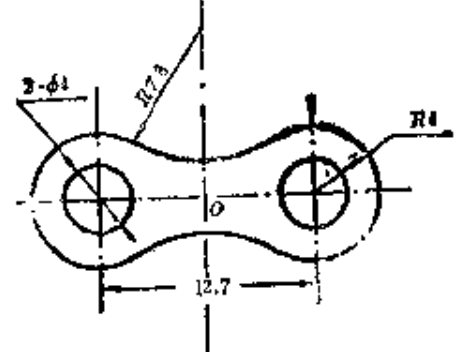
\includegraphics[width=5.5cm]{../pic/czjh2-ch7-subsec15-lx-02.png}
        \caption*{(第 2 题)}
    \end{minipage}
\end{figure}

% \begin{figure}[htbp] %
%     \centering
%     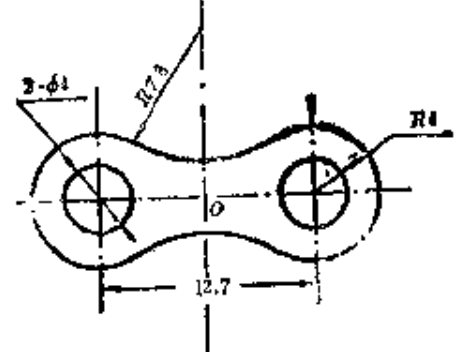
\includegraphics[width=5.5cm]{../pic/czjh2-ch7-subsec15-lx-02.png}
%     \caption*{(第 2 题)}
% \end{figure}

四条弧连接组成的图形就是椭圆的近似图形。

\begin{lianxi}

\xiaoti{说明近似椭圆的四条弧为什么是连接的。}

\xiaoti{按 $4:1$ 的比例尺,作出对应的图样。} % 原题为 “作出下面的图样”,因为排版的原因,将题目调整了一下
% 图片的代码原本应该放在这里,但由于分页时,将图片放在下一页。
% 而此后紧跟着 "习题 二十六",为了避免将此图误以为是“习题 二十六”中的图,
% 所以,将代码上移。

\end{lianxi}


\xiti
\begin{xiaotis}
\begin{enhancedline}

\xiaoti{定圆 $O$ 的半径是 4 厘米, 动圆 $P$ 的半径是 1 厘米。}
\begin{xiaoxiaotis}

    \xxt{设 $\yuan\,P$ 和 $\yuan\,O$ 相外切。 那么点 $P$ 与点 $O$ 的距离是多少? 点 $P$ 可以在什么样的线上移动?}

    \xxt{设 $\yuan\,P$ 和 $\yuan\,O$相内切呢?}

\end{xiaoxiaotis}

\xiaoti{分别以 2 厘米、2.5 厘米、4 厘米为半径作圆,使它们两两外切。}

\xiaoti{经过相交两圆的一个交点,作两圆的公共弦的垂线。求证:这条直线上被两圆所截得的线段等于圆心距的二倍。}

\xiaoti{已知: $\yuan\,O_1$ 和 $\yuan\,O_2$ 相交于点 $A$ 和 $B$,
    经过点 $A$ 的直线分别交两圆于点 $C$ 和 $D$,
    经过点 $B$ 的直线分别交两圆于点 $E$ 和 $F$, 且 $CD \pingxing EF$。求证:
}
\begin{xiaoxiaotis}

    \xxt{$CD = EF$;}

    \xxt{$CE = DF$。}

\end{xiaoxiaotis}

\xiaoti{已知: $\yuan\,O$ 和 $\yuan\,O'$ 外切于点 $A$, 经过点 $A$ 作直线 $BC$ 和 $DE$,
    $BC$ 交 $\yuan\,O$ 于点 $B$、交 $\yuan\,O'$ 于点 $C$,
    $DE$ 交 $\yuan\,O$ 于点 $D$、交 $\yuan\,O'$ 于点 $E$。
    求证: $BD \pingxing CE$。
}

\xiaoti{经过相内切的两圆的切点 $A$ 作大圆的弦 $AD$、$AE$, 设 $AD$、$AE$ 分别和小圆相交于点 $B$、$C$。
    求证:$DE \pingxing BC$; $AB:AC = AD:AE$。
}

\xiaoti{已知两个圆相外切,它们的两条外公切线互相垂直,其中大圆的半径等于 5 cm。求小圆半径及外公切线长。}

\xiaoti{$\yuan\,O_1$ 和 $\yuan\,O_2$ 相交于点 $B$ 和 $C$,
    $A$ 是 $\yuan\,O_1$ 上另一点, $AT$ 是 $\yuan\,O_1$ 的切线,
    又直线 $AB$ 与 $AC$ 分别交 $\yuan\,O_2$ 于点 $D$ 和 $E$。
    求证:$AT \pingxing DE$。
}

\xiaoti{用半径 $R = 8$ mm、 $r = 5$ mm 的钢球测量口小内大的内孔的直径 $D$。
    测得钢球顶点与孔口平面的距离分别为 $a = 12.5$ mm、$b = 8.3$ mm(如图),
    计算出内孔直径 $D$ 的大小(精确到 0.1 mm)。
}

\begin{figure}[htbp]
    \centering
    \begin{minipage}[b]{4.1cm}
        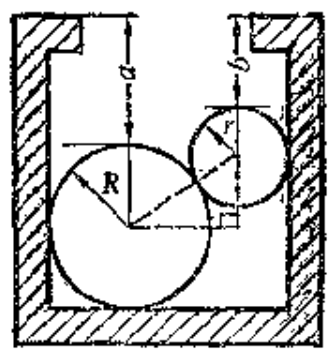
\includegraphics[width=4cm]{../pic/czjh2-ch7-xiti26-09.png}
        \caption*{}
        \caption*{(第 9 题)}
    \end{minipage}
    \qquad
    \begin{minipage}[b]{11cm}
        \begin{minipage}[b]{5.1cm}
            \centering
            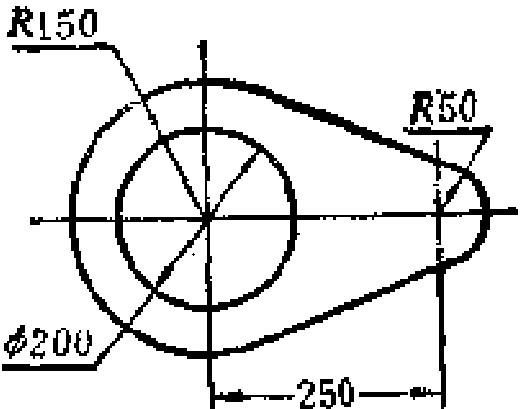
\includegraphics[width=5cm]{../pic/czjh2-ch7-xiti26-12-a.png}
            \caption*{甲}
        \end{minipage}
        \begin{minipage}[b]{5.8cm}
            \centering
            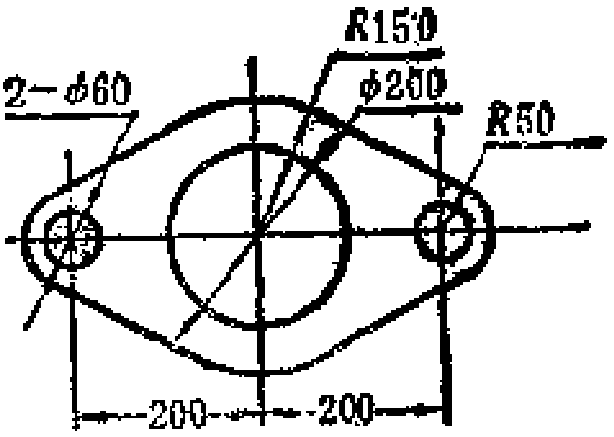
\includegraphics[width=5.7cm]{../pic/czjh2-ch7-xiti26-12-b.png}
            \caption*{乙}
        \end{minipage}
        \caption*{(第 12 题)}
    \end{minipage}
\end{figure}

\xiaoti{两圆半径为 38 mm和 22 mm, 圆心距为 65 mm。求}
\begin{xiaoxiaotis}

    \xxt{内公切线长;}

    \xxt{内公切线与连心线的夹角。}

\end{xiaoxiaotis}

\xiaoti{求证:}
\begin{xiaoxiaotis}

    \xxt{两圆的外公切线的四个切点在同一个圆上;}

    \xxt{两圆的内公切线的四个切点在同一个圆上。}
\end{xiaoxiaotis}

\xiaoti{按 $1:5$ 的比例尺,作出下列图样。}

% \begin{figure}[htbp]
%     \centering
%     \begin{minipage}[b]{7cm}
%         \centering
%         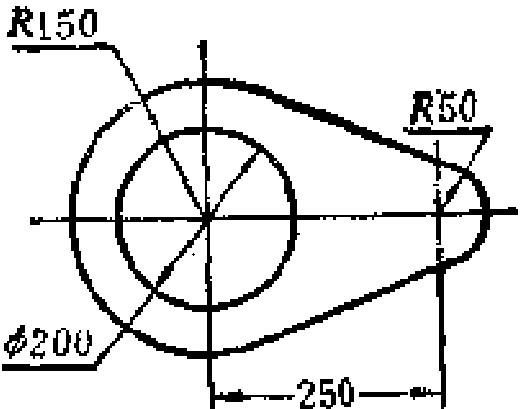
\includegraphics[width=5cm]{../pic/czjh2-ch7-xiti26-12-a.png}
%         \caption*{甲}
%     \end{minipage}
%     \begin{minipage}[b]{7cm}
%         \centering
%         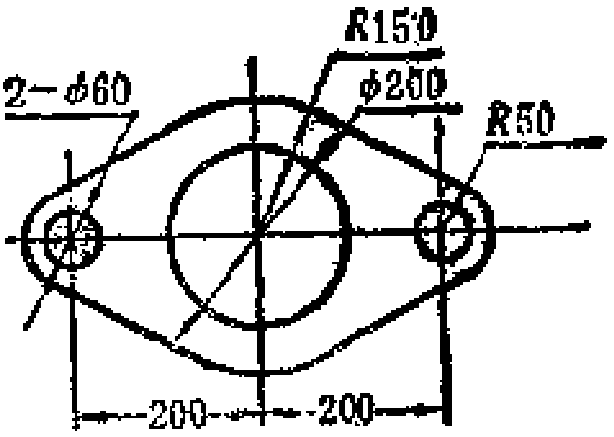
\includegraphics[width=5.7cm]{../pic/czjh2-ch7-xiti26-12-b.png}
%         \caption*{乙}
%     \end{minipage}
%     \caption*{(第 12 题)}
% \end{figure}

\xiaoti{如图, $ABCD$ 是正方形,曲线 $DEFG\cdots$ 叫做 “正方形的渐开线”。
    其中 $\yuanhu{DE}$、$\yuanhu{EF}$、$\yuanhu{FG}$、$\yuanhu{GH}$、$\cdots$
    的圆心依次按 $A$、$B$、$C$、$D$ 循环,它们依次相连接,取 $AB = 10$ mm,作图。
}

\begin{figure}[htbp]
    \centering
    \begin{minipage}[b]{7cm}
        \centering
        \begin{tikzpicture}[scale=.9] % 复杂
    \pgfmathsetmacro{\a}{0.6}

    % 绘制“正方形的渐开线”
    \tkzDefPoints{0/0/p0, -\a/0/p1, -\a/\a/p2, 0/\a/p3}
    \foreach \i in {4,5, ..., 8} {
        \pgfmathsetmacro{\o}{int(mod(\i, 4))}
        \pgfmathsetmacro{\s}{int(\i - 1)}
        \tkzDefPointBy[rotation=center {p\o} angle -90]({p\s})  \tkzGetPoint{{p\i}}
        \tkzDrawArc({p\o},{p\i})({p\s})
    }
    % 绘制最后的一小节
    \tkzDefPointBy[rotation=center p0 angle -50](p8)  \tkzGetPoint{X}
    \tkzDrawArc({p0},X)(p8)

    % 绘制正方形及其延长线
    \tkzDrawLine[add=0 and 0.2](p0, p7)
    \tkzDrawLine[add=0 and 0.2](p1, p8)
    \tkzDrawLine[add=0 and 0.2](p2, p5)
    \tkzDrawLine[add=0 and 0.2](p3, p6)

    % 显示坐标点
    \tkzLabelPoint[below](p0){$A$}
    \tkzLabelPoint[left](p1){$B$}
    \tkzLabelPoint[above](p2){$C$}
    \tkzLabelPoint[above right](p3){$D$}
    \tkzLabelPoint[below right](p4){$E$}
    \tkzLabelPoint[below right](p5){$F$}
    \tkzLabelPoint[below left](p6){$G$}
    \tkzLabelPoint[above right](p7){$H$}
    \tkzLabelPoint[below right](p8){$K$}
\end{tikzpicture}


        \caption*{(第 13 题)}
    \end{minipage}
    \qquad
    \begin{minipage}[b]{7cm}
        \centering
        \begin{tikzpicture}
    % 由各圆两两相切,得: (R - r)^2 + (R/2)^2 = (R/2 + r)^2
    % 解得: r = R/3

    % 大圆
    \pgfmathsetmacro{\R}{3}
    \tkzDefPoints{0/0/A, \R/0/O, 2*\R/0/B}
    \tkzDrawSegment[thick](A,B)
    \tkzDrawArc[very thick](O,B)(A)
    \tkzDrawPoint(O)

    % 左侧的小圆 A
    \tkzDefPoints{0.5*\R/0/O_1}
    \tkzDrawArc[very thick](O_1,O)(A)
    \tkzDrawPoint(O_1)

    % 右侧的小圆 B
    \tkzDefPoints{1.5*\R/0/O_2}
    \tkzDrawArc[very thick](O_2,B)(O)
    \tkzDrawPoint(O_2)

    % 上方的小圆 C
    \pgfmathsetmacro{\r}{\R/3}
    \tkzDefPoints{\R/\R-\r/O_3, \R/\R/C}
    \tkzDrawCircle[very thick](O_3,C)
    \tkzDrawPoint(O_3)
\end{tikzpicture}

        \caption*{(第 14 题)}
    \end{minipage}
\end{figure}

\xiaoti{已知图中各圆两两相切, 大圆半径为 $R$。求各小圆的半径,并画出图形。}

\end{enhancedline}
\end{xiaotis}



\section{正多边形和圆}
\subsection{正多边形和圆}\label{subsec:czjh2-7-16}

各边相等、各角也相等的多边形叫做\zhongdian{正多边形}。
例如等边三角形是正三角形,正方形是正四边形。
在工程技术和实用图案等方面,常常要用到正多边形(图 \ref{fig:czjh2-7-63})。
其中正三角形、正方形、正五边形、正六边形、正八边形等应用较多。

\begin{figure}[htbp]
    \centering
    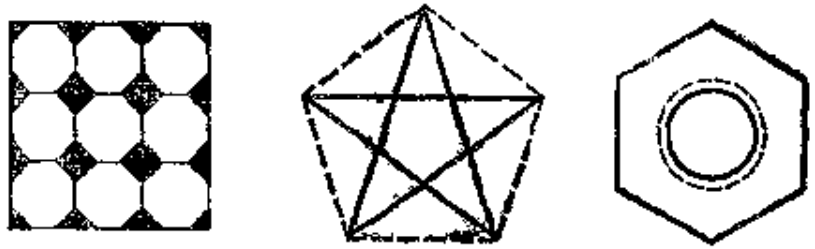
\includegraphics[width=7cm]{../pic/czjh2-ch7-63.png}
    \caption{}\label{fig:czjh2-7-63}
\end{figure}


正多边形和圆有非常密切的关系。
我们只要把一个圆分成几条相等的弧,就可以作出这个圆的内接或外切正 $n$ 边形。
下面我们来研究这个问题。

\begin{dingli}[定理]
    把圆分成 $n \; (n \geqslant 3)$ 等份:

    (1)依次连结各分点所得的多边形是这个圆的内接正 $n$ 边形;

    (2)经过各分点作圆的切线,以相邻切线的交点为顶点的多边形是这个圆的外切正 $n$ 边形。

\end{dingli}

我们以 $n = 5$ 的情况为例来进行证明。

已知: $\yuan\,O$ 中, $\yuanhu{AB} = \yuanhu{BC} = \yuanhu{CD} = \yuanhu{DE} = \yuanhu{EA}$,
$TP$、 $PQ$、$QR$、$RS$、$ST$ 分别是经过分点 $A$、$B$、$C$、$D$、$E$ 的 $\yuan\,O$ 的切线(图 \ref{fig:czjh2-7-64})。

求证:(1) 五边形 $ABCDE$ 是 $\yuan\,O$ 的内接正五边形;

(2) 五边形 $PQRST$ 是 $\yuan\,O$ 的外切正五边形。

\zhengming

(1) $\yuanhu{AB} = \yuanhu{BC} = \cdots = \yuanhu{EA}$

\quad $\tuichu \left\{\begin{aligned}
    AB = BC = \cdots = EA \\
    \yuanhu{BCE} = \yuanhu{CDA} = \cdots = \yuanhu{ABD} \quad \tuichu \quad \angle EAB = \angle ABC = \cdots = \angle DEA
\end{aligned}\right\}$

\quad $\tuichu$ 五边形 $ABCDE$ 是 $\yuan\,O$ 的内接正五边形。


(2) $\yuanhu{AB} = \yuanhu{BC} = \cdots = \yuanhu{EA}$

\quad $\tuichu \left\{\begin{aligned}
    AB = BC = \cdots = EA \\
    \angle PAB = \angle PBA = \angle QBC = \angle QCB = \cdots = \angle TEA = \angle TAE
\end{aligned}\right\}$

\quad $\tuichu$ $\triangle PAB$、$\triangle QBC$、 $\cdots$ $\triangle TEA$ 是全等的等腰三角形

\quad $\tuichu$ 五边形 $PQRST$ 是各边相等、各角相等

\quad $\tuichu$ 五边形 $PQRST$ 是 $\yuan\,O$ 的外切正五边形。

\begin{figure}[htbp]
    \centering
    \begin{minipage}[b]{7cm}
        \centering
        \begin{tikzpicture}
    \tkzDefPoints{0/0/O, 0/1.5/A}
    \tkzDrawCircle(O,A)
    \tkzDrawPoint(O)

    % 内接正五边形
    \tkzDefRegPolygon[center,sides=5,name=P](O,A)
    \tkzDrawPolygon(P1,P...,P5)
    \tkzLabelPoint[right](O){$O$}
    \tkzLabelPoint[above](P1){$A$}
    \tkzLabelPoint[left](P2){$B$}
    \tkzLabelPoint[left,  yshift=-.3em](P3){$C$}
    \tkzLabelPoint[right, yshift=-.3em](P4){$D$}
    \tkzLabelPoint[right](P5){$E$}

    % 外切正五边形
    \tkzDefLine[tangent at=P1](O)  \tkzGetPoint{p1}
    \tkzDefLine[tangent at=P2](O)  \tkzGetPoint{p2}
    \tkzInterLL(P1,p1)(P2,p2)  \tkzGetPoint{P}
    \tkzDefRegPolygon[center,sides=5,name=N](O,P)
    \tkzDrawPolygon(N1,N...,N5)
    \tkzLabelPoint[left](N1){$P$}
    \tkzLabelPoint[left](N2){$Q$}
    \tkzLabelPoint[below](N3){$R$}
    \tkzLabelPoint[right](N4){$S$}
    \tkzLabelPoint[right](N5){$T$}
\end{tikzpicture}


        \caption{}\label{fig:czjh2-7-64}
    \end{minipage}
    \qquad
    \begin{minipage}[b]{7.2cm}
        \centering
        \begin{tikzpicture}
    % 绘制已知的 正五边形
    \tkzDefPoints{0/0/A, 2/0/B}
    \tkzDefRegPolygon[side,sides=5,name=P](A,B)
    \tkzDrawPolygon[thick](P1,P...,P5)
    \coordinate (C) at (P3); % 后面还会用到这些点,所以将其命名为 C、D、E
    \coordinate (D) at (P4);
    \coordinate (E) at (P5);
    \tkzLabelPoint[left,  yshift=-.3em](A){$A$}
    \tkzLabelPoint[right, yshift=-.3em](B){$B$}
    \tkzLabelPoint[right](C){$C$}
    \tkzLabelPoint[above](D){$D$}
    \tkzLabelPoint[left](E){$E$}

    % 绘制外接圆
    \tkzDefLine[mediator](A,B)   \tkzGetPoints{a}{b}
    \tkzDefLine[mediator](C,D)  \tkzGetPoints{c}{d}
    \tkzInterLL(a,b)(c,d)  \tkzGetPoint{O}
    \tkzDrawCircle[very thick](O,A)
    \tkzLabelPoint[left](O){$O$}

    % 绘制内切圆
    \tkzDefPointBy[projection= onto A--B](O)  \tkzGetPoint{H}
    \tkzDrawCircle[very thick](O,H)

    % 其它
    \tkzDrawSegments[dashed](O,A  O,B  O,C  O,D)
    \extkzLabelAngel[0.5](C,B,O){$1$}
    \extkzLabelAngel[0.5](O,C,B){$2$}
    \extkzLabelAngel[0.7](O,B,A){$3$}
    \extkzLabelAngel[0.7](D,C,O){$4$}
\end{tikzpicture}


        \caption{}\label{fig:czjh2-7-65}
    \end{minipage}
\end{figure}

反过来,是不是每一个正多边形都有一个外接圆和一个内切圆呢?
我们仍以正五边形 $ABCDE$ 为例来研究这个问题。

经过顶点 $A$、$B$、$C$ 作 $\yuan\,O$, 连结 $OA$、$OB$、$OC$、$OD$ (图 \ref{fig:czjh2-7-65} )。

$\left.\begin{aligned}
    OB = OC \tuichu \angle 1 = \angle 2 \\
    \angle ABC = \angle BCD
\end{aligned}\right\}$

\qquad $\left.\begin{aligned}
    \tuichu \quad \angle 4 = \angle 3 \\
    OC = OB \\
    CD = BA
\end{aligned}\right\}$

\qquad $\tuichu \triangle ODC \quandeng \triangle OAB$

\qquad $\tuichu OD = OA \tuichu  $ 点 $D$ 在 $\yuan\,O$ 上。

同理,点 $E$ 在 $\yuan\,O$ 上。

所以正五边形 $ABCDE$ 有一个外接圆 $\yuan\,O$。

因为正多边形 $ABCDE$ 的各边都相等,所以它的外接圆的圆心 $O$ 到各边的距离都相等。
以 $O$ 为圆心,以这个距离为半径的圆和各边都相切。
所以,正五边形 $ABCDE$ 有一个内切圆。它的圆心就是外接圆的圆心。 于是得到:

\begin{dingli}[定理]
    任何正多边形都有一个外接圆和一个内切圆,这两个圆是同心圆。
\end{dingli}

正多边形的外接圆(或内切圆)的圆心叫做\zhongdian{正多边形的中心},
外接圆的半径叫做\zhongdian{正多边形的半径},
内切圆的半径叫做\zhongdian{正多边形的边心距}。
正多边形各边所对的外接圆的圆心角都相等。
正多边形每一边所对的外接圆的圆心角叫做\zhongdian{正多边形的中心角}。

\begin{figure}[htbp]
    \centering
    \begin{minipage}[b]{7cm}
        \centering
        \begin{tikzpicture}
    \pgfmathsetmacro{\R}{1.5}
    \pgfmathsetmacro{\n}{5} % 5 边形

    \tkzDefPoints{0/0/O}
    \tkzDefPoint(270:\R){A}
    \tkzDefRegPolygon[center,sides=\n,name=P](O,A)
    \tkzDrawPolygon(P1,P...,P\n)
    \foreach \i in {1,...,\n} {
        \tkzDrawLine[add=0.2 and 1.2](P\i,O)
    }
    \tkzLabelPoints[above, xshift=-.5em](O)
\end{tikzpicture}

% \begin{tikzpicture}
%     \tkzDefPoints{0/0/O, 0/-1.5/A}
%     \tkzDefRegPolygon[center,sides=5,name=P](O,A)
%     \tkzDrawPolygon(P1,P...,P5)
%     \foreach \i in {1,...,5} {
%         \tkzDrawLine[add=0.2 and 1.2](P\i,O)
%     }
%     \tkzLabelPoints[above, xshift=-.5em](O)
% \end{tikzpicture}


        \caption{}\label{fig:czjh2-7-66}
    \end{minipage}
    \qquad
    \begin{minipage}[b]{7cm}
        \centering
        \begin{tikzpicture}
    \pgfmathsetmacro{\R}{1.5}
    \pgfmathsetmacro{\n}{6} % 6 边形
    \pgfmathsetmacro{\halfn}{int(\n/2)} % 边数的一半。用于减少绘制时的重复动作。

    \tkzDefPoints{0/0/O}
    \tkzDefPoint(0:\R){A}
    \tkzDefRegPolygon[center,sides=\n,name=P](O,A)
    \tkzDrawPolygon(P1,P...,P\n)

    \tkzDefLine[mediator](P1,P2)   \tkzGetPoints{a}{b}
    \tkzDefLine[mediator](P3,P4)  \tkzGetPoints{c}{d}
    \tkzInterLL(a,b)(c,d)  \tkzGetPoint{O}
    \foreach \i in {1,...,\halfn} {
        \pgfmathsetmacro{\s}{int(\i + 1)}
        \tkzDefMidPoint(P\i,{P\s})  \tkzGetPoint{X}
        \tkzDrawLine[add=0.2  and 1.2](P\i,O)
        \tkzDrawLine[add=0.25 and 1.25](X,O)
    }
    \tkzLabelPoints[above, xshift=-.5em](O)
\end{tikzpicture}

% \begin{tikzpicture}
%     \tkzDefPoints{0/0/A, 1.6/0/B}
%     \tkzDefRegPolygon[side,sides=6,name=P](A,B)
%     \tkzDrawPolygon(P1,P...,P6)

%     \tkzDefLine[mediator](P1,P2)   \tkzGetPoints{a}{b}
%     \tkzDefLine[mediator](P3,P4)  \tkzGetPoints{c}{d}
%     \tkzInterLL(a,b)(c,d)  \tkzGetPoint{O}
%     \foreach \i in {1,...,3} {
%         \pgfmathsetmacro{\s}{int(\i + 1)}
%         \tkzDefMidPoint(P\i,{P\s})  \tkzGetPoint{X}
%         \tkzDrawLine[add=0.2  and 1.2](P\i,O)
%         \tkzDrawLine[add=0.25 and 1.25](X,O)
%     }
%     \tkzLabelPoints[above, xshift=-.5em](O)
% \end{tikzpicture}


        \caption{}\label{fig:czjh2-7-67}
    \end{minipage}
\end{figure}

正多边形都是轴对称图形, 一个正 $n$ 边形共有 $n$ 条对称轴,(为什么?)
每条对称轴都通过正 $n$ 边形的中心(图 \ref{fig:czjh2-7-66})。
如果正多边形有偶数条边,那么它又是中心对称图形,它的中心就是对称中心(图 \ref{fig:czjh2-7-67} )。

边数相同的正多边形相似。所以它们的周长的比等于它们的边长(或半径、边心距)的比,
它们的面积的比等于它们的边长(或半径、边心距)平方的比,


\begin{lianxi}

\xiaoti{(口答)矩形是正多边形吗?菱形是正多边形吗?为什么?}

\xiaoti{求证:}
\begin{xiaoxiaotis}

    \xxt{各边相等的圆内接多边形是正多边形;}

    \xxt{各角相等的圆外切多边形是正多边形。}

\end{xiaoxiaotis}


\begin{enhancedline}
\xiaoti{证明: 在正 $n$ 边形中,}
\begin{xiaoxiaotis}

    \xxt{中心角等于 $\dfrac{360^\circ}{n}$;}
    \xxt{中心角与外角相等。}

\end{xiaoxiaotis}

\xiaoti{(口答)一个正五边形,要绕它的中心至少转多少角度,才能和原来的正五边形重合?
    在不超过 $360^\circ$ 的范围内,这样的角度有几个? 正 $n$ 边形呢?
}
\end{enhancedline}

\end{lianxi}


\subsection{正多边形的有关计算}\label{subsec:czjh2-7-17}

\begin{enhancedline}

我们知道,多边形的内角和等于 $(n - 2) \cdot 180^\circ$。
因为正多边形的各角都相等,所以它的每个内角都等于
$$ \dfrac{(n - 2) \cdot 180}{n}  \juhao $$

下面研究正多边形的其他计算问题。

正 $n$ 边形的 $n$ 条半径把它分成了 $n$ 个等腰三角形,如图 \ref{fig:czjh2-7-68} ,
这些等腰三角形底边上的高,又把它们分成 $2n$ 个直角三角形,
而这些直角三角形的斜边恰好都是正 $n$ 边形的半径,
一条直角边是正 $n$ 边形的边心距,
另一条直角边是正 $n$ 边形边长的一半,
显然这些直角三角形是全等的。 因而得到:

\begin{figure}[htbp]
    \centering
    \begin{minipage}[b]{7cm}
        \centering
        \begin{tikzpicture}
    \pgfmathsetmacro{\R}{2}
    \pgfmathsetmacro{\n}{8}

    \tkzDefPoints{0/0/O}
    \tkzDefPoint(247.5:\R){A} % 270 - 360/8/2 = 270 - 22.5 = 247.5
    \tkzDefRegPolygon[center,sides=\n,name=P](O,A)
    \coordinate (B) at (P2);

    \tkzDefLine[altitude](A,O,B)  \tkzGetPoint{G}

    \tkzDrawCircle[very thick](O,A)
    \tkzDrawSegments(B,P3  P8,A)
    \tkzDrawSegments[dim={$a_n$,-1em,}](A,B)
    \tkzDrawSegments[dashed](O,A  O,B  O,G)

    \tkzMarkRightAngle[size=.2](B,G,O)
    \extkzLabelAngel[0.5](A,O,B){$\alpha_n$}
    \tkzLabelSegment[right](O,B){$R$}
    \tkzLabelSegment[pos=.8, left, xshift=.2em](O,G){$r_n$}
    \tkzLabelPoints[above](O)
    \tkzLabelPoints[left,  yshift=-.3em](A)
    \tkzLabelPoints[right, yshift=-.3em](B)
\end{tikzpicture}


        \caption{}\label{fig:czjh2-7-68}
    \end{minipage}
    \qquad
    \begin{minipage}[b]{7cm}
        \centering
        \begin{tikzpicture}
    \pgfmathsetmacro{\R}{2}
    \pgfmathsetmacro{\n}{6}

    \tkzDefPoints{0/0/O}
    \tkzDefPoint(240:\R){A} % 270 - 360/6/2 = 270 - 30 = 240
    \tkzDefRegPolygon[center,sides=\n,name=P](O,A)
    \foreach \P [count=\i from 2] in {B,C,...,F} {
        \coordinate (\P) at (P\i);
    }
    \tkzDefLine[altitude](A,O,B)  \tkzGetPoint{G}

    \tkzDrawCircle[very thick](O,A)
    \tkzDrawPolygon(P1,P...,P\n)
    \tkzDrawSegments[dim={$a_6$,-1.2em,}](A,B)
    \tkzDrawSegments(O,A  O,B  O,G)

    \tkzMarkRightAngle[size=.2](B,G,O)
    \tkzLabelSegment[right](O,B){$R$}
    \tkzLabelSegment[pos=.3, xshift=-.5em](O,G){$r_6$}
    \tkzLabelPoints[above](O)
    \tkzLabelPoints[left,  yshift=-.3em](A)
    \tkzLabelPoints[right, yshift=-.3em](B)
    \tkzAutoLabelPoints[center=O, centered, dist= .2](C,...,F)
    \tkzLabelPoints[above, xshift=-.5em](G)
\end{tikzpicture}


        \caption{}\label{fig:czjh2-7-69}
    \end{minipage}
\end{figure}


\begin{dingli}[定理]
    正 $n$ 边形的半径和边心距把正 $n$ 边形分成 $2n$ 个全等的直角三角形。
\end{dingli}

由于正 $n$ 边形的中心角 $\alpha_n = \dfrac{360^\circ}{n}$,我们应用上面定理,
就可以把正 $n$ 边形的边长 $a_n$, 边心距 $r_n$, 周长 $p_n$ 和面积 $S_n$
等的计算问题归结为有关直角三角形的计算问题。



\liti[0] 已知正六边形 $ABCDEF$ 的半径为 $R$,求这个正六边形的边长 $a_6$;
周长 $p_6$ 和面积 $S_6$。

\jie 连结半径 $OA$、$OB$, 作 $\triangle OAB$ 的高 $OG$,得 $Rt \triangle OGB$(图 \ref{fig:czjh2-7-69})。

$\because$ \quad $\angle GOB = \dfrac{360^\circ}{2n} = 30^\circ$,

$\therefore$ \quad $a_6 = 2 R \sin 30^\circ = 2 \cdot \exdfrac{R}{2} = R$。

$\therefore$ \quad $p_6 = 6 \cdot a_6 = 6 R$。

$\because$ \quad $r_6 = R \cos 30^\circ = \dfrac{\sqrt{3}}{2} R$,

$\therefore$ \quad $S_6 = 6 \cdot \exdfrac{1}{2} \cdot r_6 \cdot a_6 = \dfrac{3\sqrt{3}}{2} R^2$。


\begin{lianxi}

\xiaoti{已知圆的半径为 $R$,求它的内接正三角形、正方形的边长、边心距及面积。}

\xiaoti{在半径为 20 cm 的圆中,利用三角函数表,计算内接正九边形的边长、边心距、周长及面积(保留四个有效数字)。}

\xiaoti{一个正七边形的边长为 12 cm, 利用三角函数表,计算它的面积(保留三个有效数字)。}

\xiaoti{设正三角形的边长为 $a$,求它的边心距、半径和高。并证明:
    $\text{边心距} : \text{半径} : \text{高} = 1 : 2 : 3$。
}

\end{lianxi}

\end{enhancedline}

\subsection{正多边形作图}\label{subsec:czjh2-7-18}

\begin{enhancedline}

半径为 $R$ 的正多边形的作图问题,实际上是它的外接圆的等分问题。
把圆 $n$ 等分后,顺次连结各分点,就得到正 $n$ 边形。

由于正 $n$ 边形的中心角 $\alpha_n = \dfrac{360^\circ}{n}$, 使用量角器,
作出中心角 $\alpha_n$, 就可以把圆分成 $n$ 等份,从而作出半径为 $R$ 的正 $n$ 边形。

又因为正 $n$ 边形的边长 $a_n = 2 R \sin \dfrac{180^\circ}{n}$,使用正弦函数表,
可以算出半径为 $R$ 的正 $n$ 边形的边长 $a_n$,用刻度尺和圆规也可以把圆分成 $n$ 等份,
再作出半径为 $R$ 的正 $n$ 边形。 《中学数学用表》上还有 “等分圆周表”,
给出了直径为 1 的圆的内接正三角形至内接正一百边形的边长,
即给出了 $2R = 1$ 时, $n$ 为 3 ~\, 100 的 $\alpha_n$ 的值。
实际上,这些值就是 $\sin\dfrac{180^\circ}{n}$ 的值。

用上面的方法作出的正 $n$ 边形,都是近似的,但对于一些特殊的正 $n$ 边形,
还可以使用直尺和圆规来作准确的图形。

(1) 正四、八、… 边形的作法。

\begin{figure}[htbp]
    \centering
    \begin{minipage}[b]{7cm}
        \begin{tikzpicture}
    \pgfmathsetmacro{\R}{1.5}
    \tkzDefPoints{0/0/O}
    \tkzDefPoint(180:\R){A}
    \tkzDefPoint(270:\R){B}
    \tkzDefPoint(0:\R){C}
    \tkzDefPoint(90:\R){D}

    \tkzDrawCircle[very thick](O,A)
    \tkzDrawPolygon[red, thick](A,B,C,D)
    \tkzDrawSegments(A,C  B,D)
    \tkzLabelPoints[above right](O)
    \tkzLabelPoints[left](A)
    \tkzLabelPoints[below](B)
    \tkzLabelPoints[right](C)
    \tkzLabelPoints[above](D)
\end{tikzpicture}


    \end{minipage}
    \begin{minipage}[b]{7cm}
        \begin{tikzpicture}
    \pgfmathsetmacro{\R}{1.5}
    \tkzDefPoints{0/0/O}
    \tkzDefPoint(180:\R){A}
    \tkzDefPoint(270:\R){B}
    \tkzDefPoint(0:\R){C}
    \tkzDefPoint(90:\R){D}
    \tkzDefPoint(225:\R){E}
    \tkzDefPoint(315:\R){F}
    \tkzDefPoint(45:\R){G}
    \tkzDefPoint(135:\R){H}

    \tkzDrawCircle[very thick](O,A)
    \tkzDrawPolygon[red, thick](A,E,B,F,C,G,D,H)
    \tkzDrawSegments(A,C  B,D  E,G  F,H)
    \tkzLabelPoints[above=.4em, xshift=.4em](O)
    \tkzLabelPoints[left](A)
    \tkzLabelPoints[below](B)
    \tkzLabelPoints[right](C)
    \tkzLabelPoints[above](D)
    \tkzLabelPoints[below left](E)
    \tkzLabelPoints[below right](F)
    \tkzLabelPoints[above right](G)
    \tkzLabelPoints[above left](H)
\end{tikzpicture}


    \end{minipage}
    \caption{}\label{fig:czjh2-7-70}
\end{figure}


如图 \ref{fig:czjh2-7-70}, 在 $\yuan\,O$ 中,用直尺和圆规作两条互相垂直的直径,就可以作出正四边形。
再逐次作所成的中心角的平分线,还可以作出正八、十六、… 边形。

(2) 作正六、三、十二、… 边形。

\begin{figure}[htbp]
    \centering
    \begin{minipage}[b]{5cm}
        \begin{tikzpicture}
    \pgfmathsetmacro{\R}{1.5}
    \tkzDefPoints{0/0/O}
    \tkzDefPoint(240:\R){A}
    \tkzDefRegPolygon[center,sides=6,name=P](O,A)
    \foreach \P [count=\i from 2] in {B,C,...,F} {
        \coordinate (\P) at (P\i);
    }

    \tkzDrawCircle[very thick](O,A)
    \tkzDrawPolygon[red, thick](A,...,F)
    \tkzDrawSegments(C,F)
    \tkzDrawArc(F,A)(E)
    \tkzDrawArc(C,D)(B)
    \tkzLabelPoints[above right](O)
    \tkzAutoLabelPoints[center=O, centered, dist= .25](A,B,...,F)
\end{tikzpicture}

% \begin{tikzpicture}
%     \pgfmathsetmacro{\R}{1.5}
%     \tkzDefPoints{0/0/O}
%     \tkzDefPoint(0:\R){C}
%     \tkzDefPoint(60:\R){D}
%     \tkzDefPoint(120:\R){E}
%     \tkzDefPoint(180:\R){F}
%     \tkzDefPoint(240:\R){A}
%     \tkzDefPoint(300:\R){B}

%     \tkzDrawCircle[very thick](O,A)
%     \tkzDrawPolygon[red, thick](A,...,F)
%     \tkzDrawSegments(C,F)
%     \tkzDrawArc(F,A)(E)
%     \tkzDrawArc(C,D)(B)
%     \tkzLabelPoints[above right](O)
%     \tkzLabelPoints[below left](A)
%     \tkzLabelPoints[below right](B)
%     \tkzLabelPoints[right](C)
%     \tkzLabelPoints[above right](D)
%     \tkzLabelPoints[above left](E)
%     \tkzLabelPoints[left](F)
% \end{tikzpicture}


    \end{minipage}
    \begin{minipage}[b]{5cm}
        \begin{tikzpicture}
    \pgfmathsetmacro{\R}{1.5}
    \tkzDefPoints{0/0/O}
    \tkzDefPoint(240:\R){A}
    \tkzDefRegPolygon[center,sides=6,name=P](O,A)
    \foreach \P [count=\i from 2] in {B,C,...,F} {
        \coordinate (\P) at (P\i);
    }

    \tkzDrawCircle[very thick](O,A)
    \tkzDrawPolygon[red, thick](A,C,E)
    \tkzDrawPoint(O)
    \foreach \P in {B, D, F} {
        \tkzDefPointOnLine[pos=0.1](\P, O)  \tkzGetPoint{a}
        \tkzDefPointOnLine[pos=2](a, \P)  \tkzGetPoint{b}
        \tkzDrawSegment(a,b)
    }
    \tkzLabelPoints[below](O)
    \tkzAutoLabelPoints[center=O, centered, dist= .25](A,B,...,F)
\end{tikzpicture}


    \end{minipage}
    \begin{minipage}[b]{5cm}
        \begin{tikzpicture}
    \pgfmathsetmacro{\R}{1.5}
    \tkzDefPoints{0/0/O}
    \tkzDefPoint(0:\R){C}
    \tkzDefRegPolygon[center,sides=12,name=P](O,C)

    \tkzDrawCircle[very thick](O,C)
    \tkzDrawPolygon[red, thick](P1,P...,P12)
    \tkzDrawSegments[dashed](C,P7  P4,P10)
    \foreach \n in {30, 60, 120, 150, 210, 240, 300, 330} {
        \tkzDefPoint(\n:\R){P}
        \tkzDefPointOnLine[pos=0.1](P, O)  \tkzGetPoint{a}
        \tkzDefPointOnLine[pos=2](a, P)  \tkzGetPoint{b}
        \tkzDrawSegment(a,b)
    }
    \tkzLabelPoints[below left](O)
    \tkzLabelPoint[below left](P9){$A$}
    \tkzLabelPoint[below right](P11){$B$}
    \tkzLabelPoints[right](C)
\end{tikzpicture}


    \end{minipage}
    \caption{}\label{fig:czjh2-7-71}
\end{figure}

正六边形的边长 $a_6 = R$, 从图 \ref{fig:czjh2-7-71} 中容易看出,用直尺圆规可以作出正六、三、十二、… 边形。


(3) 作正十、五边形。

\begin{figure}[htbp]
    \centering
    \begin{minipage}[b]{7cm}
        \centering
        \begin{tikzpicture}
    \pgfmathsetmacro{\R}{1.5}
    \tkzDefPoints{0/0/O}
    \tkzDefPoint(0:\R){T1}
    \tkzDrawCircle[very thick](O,T1)

    \tkzDefRegPolygon[center,sides=10,name=P](O,T1)
    \tkzDrawPolygon[thick,red](P1,P...,P10)

    \coordinate (A) at (P8);
    \coordinate (B) at (P9);
    \coordinate (C) at (P10);

    \foreach \n in {-36, 0, ..., 216} {
        \tkzDefPoint(\n:\R){P}
        \tkzDefPointOnLine[pos=0.1](P, O)  \tkzGetPoint{a}
        \tkzDefPointOnLine[pos=2](a, P)  \tkzGetPoint{b}
        \tkzDrawSegment(a,b)
    }


    \tkzDefLine[bisector](O,B,A)  \tkzGetPoint{m}
    \tkzInterLL(B,m)(O,A)  \tkzGetPoint{M}
    \tkzDrawSegments[dashed](O,A  O,B  B,M)

    \tkzMarkAngle[size=.3](A,O,B)
    \tkzDefPoint(270:.3){x}
    \tkzDefShiftPoint[x](-.3,.2){y}
    \tkzDefShiftPoint[y](-.4,0){z}
    \tkzDrawSegment[green](x,y)
    \tkzDrawSegment[green,thick](y,z)
    \tkzLabelSegment[above](y,z){\small $36^\circ$}

    \tkzMarkAngle[size=.3](O,B,M)
    \tkzDefShiftPoint[B](120:.3){x}
    \tkzDefShiftPoint[x](.3,.5){y}
    \tkzDefShiftPoint[y](.4,0){z}
    \tkzDrawSegment[green](x,y)
    \tkzDrawSegment[green,thick](y,z)
    \tkzLabelSegment[above](y,z){\small $36^\circ$}

    \tkzMarkAngle[size=.2](B,A,O)
    \tkzDefShiftPoint[A](45:.2){x}
    \tkzDefShiftPoint[x](-.4,.5){y}
    \tkzDefShiftPoint[y](-.4,0){z}
    \tkzDrawSegment[green](x,y)
    \tkzDrawSegment[green,thick](y,z)
    \tkzLabelSegment[above](y,z){\small $72^\circ$}

    \tkzLabelPoints[above](O)
    \tkzLabelPoints[below](A)
    \tkzLabelPoints[below](B)
    \tkzLabelPoints[below right](C)
    \tkzLabelPoints[xshift=-.5em, yshift=1.2em](M)
\end{tikzpicture}


        \caption{}\label{fig:czjh2-7-72}
    \end{minipage}
    \qquad
    \begin{minipage}[b]{7cm}
        \centering
        \begin{tikzpicture}
    \pgfmathsetmacro{\R}{1.5}
    \pgfmathsetmacro{\halfR}{\R/2}

    \tkzDefPoints{0/0/O}
    \tkzDefPoint(270:\R){A}
    \tkzDrawCircle[very thick](O,A)

    \tkzDefRegPolygon[center,sides=10,name=P](O,A)
    \tkzDrawPolygon[thick,red](P1,P...,P10)
    \foreach \P [count=\i from 2] in {B,C,...,J} {
        \coordinate (\P) at (P\i);
    }
    \tkzAutoLabelPoints[center=O, centered, dist= .2](A,B,...,J)
    \tkzLabelPoints[above](O)

    %------ 黄金分割
    \tkzDrawSegment[dashed](O,A)

    % 1
    \tkzDefPointOnLine[pos=0.5](O,A)  \tkzGetPoint{p1}
    \tkzDefLine[perpendicular=through A](O,A)  \tkzGetPoint{p2}
    \tkzInterLC(A,p2)(A,p1)  \tkzGetFirstPoint{P}
    \tkzDrawSegment[dashed](A,P)
    \tkzLabelPoints[below](P)

    % 2
    \tkzDrawSegment[dashed](O,P)
    \tkzInterLC(O,P)(P,A)  \tkzGetFirstPoint{N}
    \tkzDrawArc[towards](P,A)(N)
    % \tkzDrawPoint(N)

    % 3
    \tkzInterLC(O,A)(O,N)  \tkzGetSecondPoint{M}
    \tkzDrawArc[towards](O,N)(M)
    \tkzDrawPoint(M)
    \tkzLabelPoints[right](M)
\end{tikzpicture}


        \caption{}\label{fig:czjh2-7-73}
    \end{minipage}
\end{figure}

假设正十边形已经作出,如图 \ref{fig:czjh2-7-72}, $AB$ 是 $\yuan\,O$ 内接正十边形的一边,
连结 $OA$、$OB$ 得到顶角 $\alpha_{10} = 36^\circ$,
底角为 $\dfrac{180^\circ - 36^\circ}{2} = 72^\circ$ 的等腰三角形 $OAB$,
作底角的平分线 $BM$ 交 $OA$ 于 $M$, 可得到 $\angle ABM = \angle MBO = \angle AOB = 36^\circ$,
所以 $OM = MB$。 由 $\angle AMB = \angle MAB = 72^\circ$,得 $MB = AB$, 所以 $OM = AB$。
因为 $\triangle OAB \xiangsi \triangle BAM$, 得到 $OA : AB = BA : AM$,即
$$ OA : OM = OM : AM \juhao $$
所以 $M$ 是半径 $OA$ 的黄金分割点, $OM$ 等于正十边形的边长。

把圆的半径 $OA$ 作黄金分割, 如图 \ref{fig:czjh2-7-73}, $OM$ 就等于正十边形的边长。
以 $OM$ 为半径作弧等分圆周,顺次连结各分点,就得到正十边形 $ABC\cdots J$。

图 \ref{fig:czjh2-7-73} 中, 分点 $A$、$C$、$E$、$G$、$I$ 把 $\yuan\,O$ 分成 5 等份。
顺次连结各点,就得正五边形 $ACEGI$。

把圆分成 5 等份,还可以用下面作法:

如图 \ref{fig:czjh2-7-74} 甲,作已知圆 $O$ 的互相垂直的直径 $XY$ 和 $AZ$;取半径 $OX$ 的中点 $M$;
以 $M$ 为圆心, $MA$ 为半径作弧 $\yuanhu{AN}$, 和半径 $OY$ 相交于 $N$;
在 $\yuan\,O$ 上连续截取等弧, 使弦 $AB = BC = CD = DE = AN$;
则 $A$、$B$、$C$、$D$、$E$ 就是所求作的分点。

把圆分成了 5 等份,还可以作出如图 \ref{fig:czjh2-7-74} 乙所示的正五角星形。

\begin{figure}[htbp]
    \centering
    \begin{minipage}[b]{10cm}
        \centering
        \begin{minipage}[b]{5cm}
            \centering
            \begin{tikzpicture}
    \pgfmathsetmacro{\R}{1.5}
    \tkzDefPoints{0/0/O}
    \tkzDefPoint(90:\R){A}
    \tkzDefRegPolygon[center,sides=5,name=P](O,A)
    \foreach \P [count=\i from 2] in {E,D,...,B} {
        \coordinate (\P) at (P\i);
    }
    \tkzDefPoint(180:\R){X}
    \tkzDefPoint(0:\R){Y}
    \tkzDefPoint(270:\R){Z}

    \tkzDrawCircle[very thick](O,A)
    \tkzDrawPolygon[red, thick](A,B,...,E)
    \tkzDrawSegments(A,Z  X,Y)
    \tkzMarkRightAngle[size=.2](A,O,X)

    \tkzLabelPoints[above right](O)
    \tkzAutoLabelPoints[center=O, centered, dist= .25](A,B,...,E,X,Y,Z)

    %
    \tkzDefMidPoint(O,X)  \tkzGetPoint{M}
    \tkzInterLC(O,Y)(M,A)  \tkzGetSecondPoint{N}
    \tkzDrawSegment[dashed](M,A)
    \tkzDrawArc(M,N)(A)
    \tkzLabelPoints[below](M,N)

    % \tkzInterCC(A,N)(O,A)  \tkzGetFirstPoint{B}
    \tkzDrawSegment[dashed](A,N)
    \tkzDrawArc(A,N)(B)
\end{tikzpicture}


            \caption*{甲}
        \end{minipage}
        \begin{minipage}[b]{4.5cm}
            \centering
            \begin{tikzpicture}
    \pgfmathsetmacro{\R}{1.5}
    \tkzDefPoints{0/0/O}
    \tkzDefPoint(90:\R){A}
    \tkzDefRegPolygon[center,sides=5,name=P](O,A)
    \foreach \P [count=\i from 2] in {E,D,...,B} {
        \coordinate (\P) at (P\i);
    }

    \tkzDrawCircle[very thick](O,A)
    \tkzDrawPolygon[red, thick](A,C,E,B,D)

    \tkzDefPoint(270:\R){Z}
    \tkzLabelPoints[white,below](Z)
\end{tikzpicture}


            \caption*{乙}
        \end{minipage}
        \caption{}\label{fig:czjh2-7-74}
    \end{minipage}
    \begin{minipage}[b]{4.5cm}
        \centering
        \begin{tikzpicture}
    \pgfmathsetmacro{\R}{1.5}
    \tkzDefPoints{0/0/O}
    \tkzDefPoint(90:\R){A}
    \tkzDefRegPolygon[center,sides=6,name=P](O,A)
    \foreach \P [count=\i from 2] in {B,C,...,F} {
        \coordinate (\P) at (P\i);
    }
    \tkzLabelPoints[above, xshift=.5em](O)
    \tkzAutoLabelPoints[center=O, centered, dist= .25](A,B,...,F)

    % 1
    \tkzDefPoint(180:\R){M}
    \tkzDefPoint(0:\R){N}
    \tkzDrawCircle[very thick](O,A)
    \tkzDrawSegments(A,D  M,N)
    \tkzLabelPoints[above, xshift=.6em](M)
    \tkzLabelPoints[below, xshift=-.6em](N)

    % 2
    \tkzInterLL(D,B)(M,N)  \tkzGetPoint{O_1}
    \tkzInterLL(D,F)(M,N)  \tkzGetPoint{O_2}
    \tkzDrawSegments(D,B  D,F)
    \tkzLabelPoints[above, xshift=.4em](O_1)
    \tkzLabelPoints[above, xshift=-.4em](O_2)

    % 3
    \tkzCalcLength(O_1,B)    \tkzGetLength{rOB}
    \tkzDrawArc[red, thick, R with nodes](O_1,\rOB)(B,C)  %\tkzDrawArc(O_1,B)(C)
    \tkzDrawArc[red, thick, R with nodes](O_2,\rOB)(E,F)  %\tkzDrawArc(O_2,E)(F)

    \tkzCalcLength(D,B)    \tkzGetLength{rDB}
    \tkzDrawArc[red, thick, R with nodes](A,\rDB)(C,E)
    \tkzDrawArc[red, thick, R with nodes](D,\rDB)(F,B)
\end{tikzpicture}


        \caption*{}
        \caption*{(第 3 题)}
    \end{minipage}
\end{figure}


\begin{lianxi}

\xiaoti{运用量角器作半径 $R = 4$ 厘米的正七边形和正九边形。
    再运用三角函数表计算出它们的边长,进行检验。
}

\xiaoti{按照图 \ref{fig:czjh2-7-74} 甲所示的作法,在半径为 3 厘米的圆中作出如图 \ref{fig:czjh2-7-74} 乙所示的正五角星形。}

\xiaoti{如图画近似椭圆。 先将 $\yuan\,O$ 六等分,分点为 $A$、$B$、$C$、$D$、$E$、$F$,
    作互相垂直的直径 $AD$、$MN$, 连结 $DB$、$DF$ 与 $MN$ 分别相交于 $O_1$、$O_2$,
    分别以 $O_1$、$O_2$ 为圆心,以 $O_1B$ 为半径作 $\yuanhu{BC}$、$\yuanhu{EF}$;
    分别以 $A$、$D$ 为圆心, 以 $DB$ 为半径作 $\yuanhu{CE}$、$\yuanhu{BF}$,
    四条环连接成一个椭圆。
}

\end{lianxi}

\end{enhancedline}

\subsection{圆周长、弧长}\label{subsec:czjh2-7-19}

\begin{enhancedline}

\subsubsection{圆周长}

我们知道,圆周长 $C$ 与半径 $R$ 之间有下面的关系

\begin{center}
    \framebox[8em]{\zhongdian{$\bm{C = 2 \pi R$}。}}
\end{center}

这里 $\pi = 3.14159\cdots$, 这个无限不循环小数叫做\zhongdian{圆周率}(详见\hyperref[sec:czjh2-7-fulu]{附录})。

\subsubsection{弧长}

\begin{wrapfigure}[8]{r}{7.5cm}
    \centering
    \begin{tikzpicture}
    \pgfmathsetmacro{\factor}{.025}

    \tkzDefPoints{0/0/O}
    \foreach \n [count=\i] in {110, 90, 70} {
        \ifnum\i=2\relax
            \def\linestyle{densely dash dot}
        \else
            \def\linestyle{very thick}
        \fi

        \pgfmathsetmacro{\R}{\n*\factor}

        \tkzDefPoint(40:\R){A\i}
        \tkzDefPoint(140:\R){B\i}
        \tkzDrawArc[\linestyle](O,A\i)(B\i)

        \tkzDefLine[perpendicular=through A\i, normed](A\i,O)  \tkzGetPoint{c\i}
        \tkzDefPointOnLine[pos=70*\factor](A\i,c\i)  \tkzGetPoint{C\i}
        \tkzDrawSegment[\linestyle](A\i,C\i)

        \tkzDefLine[perpendicular=through B\i, normed](O,B\i)  \tkzGetPoint{d\i}
        \tkzDefPointOnLine[pos=70*\factor](B\i,d\i)  \tkzGetPoint{D\i}
        \tkzDrawSegment[\linestyle](B\i,D\i)
    }
    \tkzDrawSegments[very thick](C3,C1  D3,D1)

    %
    \tkzLabelPoints[below](O)
    \extkzLabelAngel[0.5](A2,O,B2){$100^\circ$}
    \tkzDrawSegment[-Latex](O,A2)
    \tkzLabelSegment[pos=.4, rotate=45](O,A2){$R\;90$}

    \tkzDefPoint(90:90*\factor){l}
    \tkzLabelPoints[centered, fill=white, inner sep=1pt](l)

    \tkzDrawLines[add=0 and 0.2](O,A1   O,B1)
    \tkzDrawLines[add=0 and 0.5](C3,C1  D3,D1)

    \tkzDrawSegments[sloped, dim={$70$,1em,}](A1,C1)
    \tkzDrawSegments[sloped, dim={$70$,1em,}](D1,B1)
\end{tikzpicture}


    \caption{}\label{fig:czjh2-7-75}
\end{wrapfigure}

因为 $360^\circ$ 的圆心角所对的弧长就是圆周长 $C = 2 \pi R$,
所以 $1^\circ$ 的圆心角所对的弧长是 $\dfrac{2 \pi R}{360}$,即 $\dfrac{\pi R}{180}$。
这样,我们就得到,半径为 $R$ 的圆中, $n^\circ$ 的圆心角所对的弧长 $l$ 的计算公式:
$$ \bm{l = \dfrac{n \pi R}{180}} \juhao $$

\liti 弯制管道时,先按中心线计算“展直长度”,再下料。
试计算图 \ref{fig:czjh2-7-75} 所示管道的展直长度 $L$ (单位:mm)。

\jie 由弧长公式,得

$l = \dfrac{100 \times 90 \times \pi}{180} = 50 \pi \approx 157$ (mm) 。

所要求的展直长度

$L = 2 \times 70 + 157 = 297$ (mm)。

答:管道的展直长度为 297 mm。



\liti 如图 \ref{fig:czjh2-7-76}, 两个皮带轮的中心距离为 2.1 m, 直径分别为 0.65 m 和 0.24 m。
(1) 求皮带长; (2)如果小轮每分转 750 转,求大轮每分转多少转。

\jie (1) 作过切点的半径 $O_1A$、$O_1D$、$O_2B$、$O_2C$, 作 $O_2E \perp O_1A$,垂足为 $E$。

$\because$ \quad $O_1A = \exdfrac{1}{2} \times 0.65 = 0.325$,
    $AE = O_2B = \exdfrac{1}{2} \times 0.24 = 0.12$, $O_1O_2 = 2.1$,

$\therefore$ \quad $O_1E = O_1A - AE = 0.325 - 0.12 = 0.205$。

$\therefore$ \quad $AB = O_2E = \sqrt{O_1O_2^2 - O_1E^2} \approx 2.090$ (m)。

$\because$ \quad $\cos\alpha = \dfrac{O_1E}{O_1O_2} \approx 0.0976$, $\angle\alpha \approx 84.4^\circ$,

$\therefore$ \quad $\angle\alpha_1 = 360^\circ - 2 \angle\alpha = 191.2^\circ$。

$\therefore$ \quad $\yuanhu{AmD}$  的长 $l_1 = \dfrac{191.2 \times \pi \times 0.325}{180} \approx 1.085$ (m)。

$\because$ \quad $\angle \alpha_2 = 360^\circ - \angle \alpha_1 = 168.8^\circ$,

$\therefore$ \quad $\yuanhu{BnC}$ 的长 $l_2 = \dfrac{168.8 \times \pi \times 0.12}{180} \approx 0.354$ (m)。

$\therefore$ \quad 皮带长 $l = l_1 + l_2 + 2 AB = 5.62$ (m)。

(2) 大轮每分的转数为

\qquad $n = \dfrac{0.12 \times 750}{0.325} \approx 277$ (转)。

答:皮带长 5.62 m, 大轮每分转 277 转。

\begin{figure}[htbp]
    \centering
    \begin{minipage}[b]{10.5cm}
        \centering
        \begin{tikzpicture}
    \pgfmathsetmacro{\factor}{.03}
    \pgfmathsetmacro{\R}{65*\factor}
    \pgfmathsetmacro{\r}{24*\factor}
    \pgfmathsetmacro{\Oo}{210*\factor}

    \tkzDefPoints{0/0/O1, \Oo/0/O2}
    \tkzDefCircle[R](O1,\R)  \tkzGetPoint{o1}
    \tkzDefCircle[R](O2,\r)  \tkzGetPoint{o2}
    \tkzDefSimilitudeCenter[ext](O1,o1)(O2,o2)  \tkzGetPoint{J}
    \tkzDefLine[tangent from = J](O1,o1)  \tkzGetPoints{D}{A}
    \tkzDefLine[tangent from = J](O2,o2)  \tkzGetPoints{C}{B}
    \tkzDefLine[altitude](A,O2,O1)  \tkzGetPoint{E}

    \tkzDrawCircle[very thick](O1, o1)
    \tkzDrawCircle[very thick](O2, o2)
    \tkzDrawSegments[thick](A,B  C,D)
    \tkzDrawSegments[dashed](O1,A  O1,D  O2,B  O2,C  O2,E  O1,O2)

    \extkzLabelAngel[0.5](O2,O1,A){$\alpha$}

    % \extkzLabelAngel[0.7](A,O1,D){$\alpha_1$}
    \tkzMarkAngle[size=0.7, latex-latex](A,O1,D)
    \tkzLabelAngle[pos=.7, fill=white, inner sep=1pt](A,O1,D){$\alpha_1$}

    %\extkzLabelAngel[0.4](C,O2,B){$\alpha_2$}
    \tkzMarkAngle[size=0.4, latex-latex](C,O2,B)
    \tkzLabelAngle[pos=.4, fill=white, inner sep=1pt](C,O2,B){$\alpha_2$}

    \tkzLabelPoints[above](A,B)
    \tkzLabelPoints[below](C,D)
    \tkzLabelPoints[left](E)
    \tkzLabelPoints[below right](O1)
    \tkzLabelPoints[above, xshift=-.6em](O2)

    \tkzDefPoint(180:\R){m}
    \tkzDefShiftPoint[O2](0:\r){n}
    \tkzLabelPoints[left](m)
    \tkzLabelPoints[right](n)
\end{tikzpicture}


        \caption{}\label{fig:czjh2-7-76}
    \end{minipage}
    \begin{minipage}[b]{5cm}
        \centering
        \begin{tikzpicture}
    \pgfmathsetmacro{\R}{2}
    \pgfmathsetmacro{\r}{1}

    \tkzDefPoints{0/0/O_1, 0/-\r/O_2}
    \tkzDefPoint(270:\R){A}
    \tkzDefPoint(235:\R){C}
    \tkzInterLC[common=O_1](O_1,C)(O_2,A)  \tkzGetFirstPoint{B}

    \tkzDrawCircle[thick](O_1,A)
    \tkzDrawCircle[thick](O_2,A)
    \tkzDrawPoints(O_2)
    \tkzDrawSegments(O_1,A  O_1,C)
    \tkzLabelPoints[above](O_1)
    \tkzLabelPoints[right](O_2)
    \tkzAutoLabelPoints[center=O_1, centered, dist= .15](A,C)
    \tkzLabelPoints[left, yshift=.3em](B)
\end{tikzpicture}


        \caption*{(第 2 题)}
    \end{minipage}
\end{figure}


\begin{lianxi}

\xiaoti{求半径为 46.0 厘米的 $18^\circ 30'$ 的弧长 $l$ (保留 3 个有效数字)。}

\xiaoti{如图,大圆 $O_1$ 的半径 $O_1A$ 是小圆 $O_2$ 的直径,
    $\yuan\,O_1$ 的半径 $O_1C$ 交 $\yuan\,O_2$ 于点 $B$。
    求证: $\yuanhu{AB}$ 和 $\yuanhu{AC}$ 的长相等。
}

\end{lianxi}

\end{enhancedline}


\subsection{圆、扇形、弓形的面积}\label{subsec:czjh2-7-20}

\begin{enhancedline}

\subsubsection{圆面积}

我们知道,圆面积 $S$ 与半径 $R$ 之间有下面的关系(详见\hyperref[sec:czjh2-7-fulu]{附录}):

\begin{center}
    \framebox[8em]{\zhongdian{$\bm{S = \pi R^2$}。}}
\end{center}


\subsubsection{扇形面积}

\begin{wrapfigure}[8]{r}{5cm}
    \centering
    \begin{tikzpicture}
    \pgfmathsetmacro{\R}{1.5}

    \tkzDefPoints{0/0/O}
    \tkzDefPoint(270:\R){A}
    \tkzDefPoint(230:\R){B}
    \tkzDefPoint(310:\R){C}

    \tkzDrawCircle[very thick](O,B)
    \tkzDrawSector[pattern={mylines[angle=55, distance={4pt}]}](O,B)(C)
    \tkzDrawLines[add=0 and 0.3](O,B  O,C)
    \tkzMarkAngle[size=0.7, latex-latex](B,O,C)
    \tkzLabelAngle[pos=.7, fill=white, inner sep=0pt](B,O,C){$n^\circ$}
    \tkzMarkAngle[size=1.8, latex-latex](B,O,C)
    \tkzLabelAngle[pos=1.8, fill=white, inner sep=0pt](B,O,C){$l$}
    \tkzLabelSegment[right](O,C){$R$}

    \tkzLabelPoints[above](O)
    \tkzLabelPoints[above](A)
    \tkzLabelPoints[left=.3em](B)
    \tkzLabelPoints[right=.3em](C)
\end{tikzpicture}


    \caption{}\label{fig:czjh2-7-77}
\end{wrapfigure}


一条弧和经过这条弧的端点的两条半径所组成的图形叫做\zhongdian{扇形}。

在半径为 $R$ 的圆中,因为圆心角是 $360^\circ$ 的扇形面积就是圆面积 $S = \pi R^2$,
所以圆心角是 $1^\circ$ 的扇形面积是 $\dfrac{\pi R^2}{360}$。
这样,在半径为 $R$ 的圆中(图 \ref{fig:czjh2-7-77}), 圆心角为 $n^\circ$ 的扇形面积的计算公式是
$$ S_\text{扇形} = \dfrac{n}{360} \pi R^2 \juhao $$

又因为,扇形的弧长 $l = \dfrac{n \pi R}{180}$, 扇形面积 $\dfrac{n}{360} \pi R^2$
可以写成 $\exdfrac{1}{2} \cdot \dfrac{n \pi R}{180} \cdot R$, 所以,又得到
$$ S_\text{扇形} = \exdfrac{1}{2} l R \juhao $$


\subsubsection{弓形面积}

从图 \ref{fig:czjh2-7-78} 中可以看出,把扇形 $OAmB$ 的面积以及 $\triangle OAB$ 的面积计算出来,
就可以得到弓形 $AmB$ 的面积。

\begin{figure}[htbp]
    \centering
    \begin{minipage}[b]{5cm}
        \begin{tikzpicture}
    \pgfmathsetmacro{\R}{1.5}

    \tkzDefPoints{0/0/O}
    \tkzDefPoint(220:\R){A}
    \tkzDefPoint(320:\R){B}
    \tkzDefPoint(270:\R){m}

    \tkzDrawSegment[very thick](A,B)
    \tkzDrawArc[very thick, pattern={mylines[angle=55, distance={4pt}]}](O,A)(B)
    \tkzDrawArc[dashed](O,B)(A)
    \tkzDrawSegments[dashed](O,A  O,B)

    \tkzLabelPoints[above](O)
    \tkzLabelPoints[below](m)
    \tkzLabelPoints[left=.3em](A)
    \tkzLabelPoints[right=.3em](B)
\end{tikzpicture}


    \end{minipage}
    \begin{minipage}[b]{5cm}
        \begin{tikzpicture}
    \pgfmathsetmacro{\R}{1.5}

    \tkzDefPoints{0/0/O}
    \tkzDefPoint(140:\R){A}
    \tkzDefPoint(40:\R){B}
    \tkzDefPoint(270:\R){m}

    \tkzDrawSegment[very thick](A,B)
    \tkzDrawArc[very thick, pattern={mylines[angle=55, distance={4pt}]}](O,A)(B)
    \tkzDrawArc[dashed](O,B)(A)
    \tkzDrawSegments[dashed](O,A  O,B)

    \tkzLabelPoints[below](O)
    \tkzLabelPoints[below](m)
    \tkzLabelPoints[left=.3em](A)
    \tkzLabelPoints[right=.3em](B)
\end{tikzpicture}


    \end{minipage}
    \begin{minipage}[b]{5cm}
        \begin{tikzpicture}
    \pgfmathsetmacro{\R}{1.5}

    \tkzDefPoints{0/0/O}
    \tkzDefPoint(180:\R){A}
    \tkzDefPoint(0:\R){B}
    \tkzDefPoint(270:\R){m}

    \tkzDrawSegment[very thick](A,B)
    \tkzDrawArc[very thick, pattern={mylines[angle=55, distance={4pt}]}](O,A)(B)
    \tkzDrawArc[dashed](O,B)(A)
    \tkzDrawPoint(O)

    \tkzLabelPoints[above](O)
    \tkzLabelPoints[below](m)
    \tkzLabelPoints[left=.3em](A)
    \tkzLabelPoints[right=.3em](B)
\end{tikzpicture}


    \end{minipage}
    \caption{}\label{fig:czjh2-7-78}
\end{figure}

\liti[0] 水平放着的圆柱形排水管的截面半径是 12 cm,其中水面高为 6 cm,
求截面上有水的弓形的面积(精确到 $1\,\pflm$)。

\begin{wrapfigure}[8]{r}{5cm}
    \centering
    \begin{tikzpicture}
    \pgfmathsetmacro{\R}{1.5}

    \tkzDefPoints{0/0/O}
    \tkzDefPoint(210:\R){A}
    \tkzDefPoint(330:\R){B}
    \tkzDefPoint(270:\R){C}
    \tkzInterLL(A,B)(O,C)  \tkzGetPoint{D}

    \tkzDrawCircle[very thick](O,A)
    \tkzDrawArc[very thick, pattern={mylines[angle=55, distance={4pt}]}](O,A)(B)
    \tkzDrawSegments[very thick](A,B  O,C)
    \tkzDrawSegments[dashed](O,A  O,B)
    \tkzMarkRightAngle[size=.2](B,D,O)

    \tkzLabelPoints[above](O)
    \tkzLabelPoints[left](A)
    \tkzLabelPoints[above right](B)
    \tkzLabelPoints[below](C)
    \tkzLabelPoints[above left](D)

    \tkzDefPointOnLine[pos=1.5](D,B)  \tkzGetPoint{b}
    \tkzDefPointBy[translation=from D to b](C)  \tkzGetPoint{c}
    \tkzDefShiftPoint[b](0,.5){b'}
    \tkzDefShiftPoint[c](0,-.5){c'}

    \tkzLabelSegment[above, rotate=30](O,A){\small 12cm}

    \tkzDrawLines[add=0 and 0.1](D,b  C,c)
    \tkzDrawSegments[-Latex](b',b  c',c)
    \tkzLabelSegment[centered, rotate=90](c,b){\small 6cm}
\end{tikzpicture}


    \caption{}\label{fig:czjh2-7-79}
\end{wrapfigure}


\jie 如图 \ref{fig:czjh2-7-79}, 连结 $OA$、$OB$, 作弦 $AB$ 的垂直平分线 $OD$,
垂足为 $D$, 交 $\yuanhu{AB}$ 于点 $C$。已知半径 $OA = 12$ cm,
$DC = 6$ cm。 那么

$OD = OC - DC = 12 - 6 = 6$ (cm),

$AD = \sqrt{OA^2 - OD^2} = \sqrt{12^2 - 6^2} = 6\sqrt{3}$ (cm),

$\angle AOD = 60^\circ$。

$\begin{aligned}
    S_{\text{弓形}ACB} &= S_{\text{扇形}OACB} - S_{\triangle OAD} \\
        &= \dfrac{120}{360} \times \pi \times 12^2 - \exdfrac{1}{2} \times 12\sqrt{3} \times 6 \\
        &= 48 \pi - 36\sqrt{3} \approx 88 (\pflm) \juhao
\end{aligned}$

答: 截面上有水的弓形的面积约为 $88\,\pflm$。


\begin{lianxi}

\xiaoti{设圆周长为 $C$, 圆面积为 $S$。 求证: $S = \dfrac{C^2}{4 \pi}$。}

\xiaoti{已知扇形的圆心角为 $150^\circ$, 弧长为 $20 \pi$ cm。求扇形的面积。}

\xiaoti{在本节的例中,设水面高为 7 cm, 其他条件不变, 利用三角函数解同样的问题。}

\end{lianxi}

\end{enhancedline}


\xiti
\begin{xiaotis}
\begin{enhancedline}

\xiaoti{求证:顺次连结正多边形各边中点所得的多边形是正多边形。}

\xiaoti{求证:正五边形的对角线相等。}

\xiaoti{求证:如果一个多边形有一个外接圆和一个内切圆,并且这两个圆是同心圆,那么这个多边形是正多边形。}

\xiaoti{已知: $AB$ 是 $\yuan\,O$ 的内接正六边形的一边,
    $AD$ 是 $\yuan\,O$ 的内接正十边形的一边,点 $D$ 在 $\yuanhu{AB}$ 上。
    求证: $DB$ 是 $\yuan\,O$ 的内接正十五边形的一边。
}

\xiaoti{求证:两个同边数的正多边形周长的比等于它们的外接圆直径的比。}

\xiaoti{在某个圆形盖板上钻 16 个等距离的小圆孔,使孔心和盖板中心的距离为 240 mm。
    求相邻两孔中心的距离(精确到 0.1 mm)。
}

\xiaoti{要用圆形铁片截出边长为 $a$ 的正方形铁片,选用的圆铁片的直径最小要多长?}

\xiaoti{如图,正六边形的螺帽的边长 $a = 12$ mm,这个搬手的开口 $b$ 最小应是多少?}

\begin{figure}[htbp]
    \centering
    \begin{minipage}[b]{7cm}
        \centering
        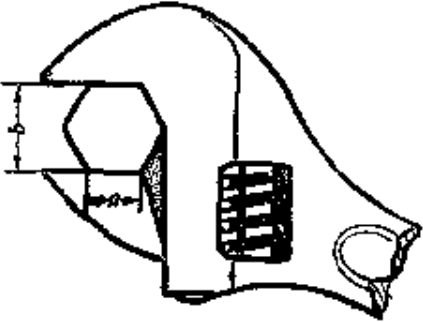
\includegraphics[width=5cm]{../pic/czjh2-ch7-xiti27-08.png}
        \caption*{(第 8 题)}
    \end{minipage}
    \begin{minipage}[b]{7cm}
        \centering
        \begin{tikzpicture}[scale=.7]
    \pgfmathsetmacro{\r}{0.2}

    % 设小圆的圆心为 O, OD 垂直于 O_1O_2, 垂足为 D。
    % 则,在直角三角形 DOO_1
    % OO1 = R + r
    % 因为:DO_1O = 30 度,所以, OD = OO1/2 = (R + r)/2
    %   R^ + [(R + r)/2]^2 = (R + r)^2
    % 化简得
    %   R^2 - 6Rr - 3r^2 = 0
    % 代入 r = 0.2 得
    %   R = 1.29
    \pgfmathsetmacro{\R}{1.29}

    \tkzDefPoints{0/0/O}
    \tkzDefPoint(210:\R+\r){O_1}
    \tkzDefPoint(330:\R+\r){O_2}
    \tkzDefPoint(90:\R+\r){O_3}

    \tkzDefCircle[R](O,\r)  \tkzGetPoint{o}
    \tkzDrawCircle[very thick](O, o)
    \foreach \n in {1,2,3} {
        \tkzDefCircle[R](O_\n,\R)  \tkzGetPoint{o_\n}
        \tkzDrawCircle[very thick](O_\n, o_\n)
    }
    \tkzDrawPolygon[dashed](O_1,O_2,O_3)
    \tkzDrawSegments[dashed](O,O_1)

    \tkzLabelPoints[left](O_1)
    \tkzLabelPoints[right](O_2)
    \tkzLabelPoints[above](O_3)
\end{tikzpicture}


        \caption*{(第 11 题)}
    \end{minipage}
\end{figure}

\xiaoti{已知圆内接正 $n$ 边形的边长为 $a$。 求同圆外切正 $n$ 边形的边长(用三角函数表示)。}

\xiaoti{求证:同一个圆的内接正六边形和外切正六边形的周长的比等干 $\sqrt{3}:2$,面积的比等于 $3:4$。}

\xiaoti{设计三个直径相等的轧辊,使它们能够把直径为 0.4 mm 的滚轴轧紧(如图)。求轧辊直径(精确到 0.01 mm)。}

\xiaoti{已知:半径为 $R$ 的圆内接正 $n$ 边形的边长为 $a_n$。
    求证:同圆内接正 $2n$ 边形的面积等于 $\exdfrac{1}{2}n R a_n$。
    利用这个结果, 求半径为 $R$ 的圆内接正八边形的面积(用代数式表示)。
}

\xiaoti{半径为 5 cm 的圆上有 10 个点,相邻两点的距离相等。
    采用如图所示的直角坐标系,求各点的坐标(精确到 0.01 cm)。
}

\begin{figure}[htbp]
    \centering
    \begin{minipage}[b]{7cm}
        \centering
        \begin{tikzpicture}
    \pgfmathsetmacro{\R}{1.5}
    \pgfmathsetmacro{\n}{10}

    \tkzDefPoints{0/0/O}
    \tkzDefPoint(0:\R){A}
    \tkzDefPoint(90:\R){Y1}
    \tkzDefPoint(270:\R){Y2}
    \tkzDefRegPolygon[center,sides=\n,name=P](O,A)
    \foreach \P [count=\i from 2] in {B,...,H,K,L} {
        \coordinate (\P) at (P\i);
    }

    \tkzDrawCircle[very thick](O,A)
    \tkzDrawPoints(P1,P...,P\n)
    \tkzDrawLines[-Latex, add=0.2 and 0.3](F,A  Y2,Y1)

    \tkzLabelPoints[below left](O)
    \tkzLabelPoints[above right](A)
    \tkzLabelPoints[below left](F)
    \tkzAutoLabelPoints[center=O, centered, dist= .2](B,...,E,G,H,K,L)
    \tkzLabelSegment[above, pos=1.25](F,A){$x$}
    \tkzLabelSegment[right, pos=1.25](Y2,Y1){$y$}
\end{tikzpicture}


        \caption*{(第 13 题)}
    \end{minipage}
    \begin{minipage}[b]{7cm}
        \centering
        \begin{tikzpicture}
    \pgfmathsetmacro{\R}{1.5}
    \pgfmathsetmacro{\n}{5}

    \tkzDefPoints{0/0/O}
    \tkzDefPoint(234:\R){A} % 90 + 360/5*2
    \tkzDefRegPolygon[center,sides=\n,name=P](O,A)
    \foreach \P [count=\i from 2] in {B,...,E} {
        \coordinate (\P) at (P\i);
    }
    \tkzInterLL(A,C)(B,E)  \tkzGetPoint{M}

    \tkzDrawPolygon[thick](A,...,E)
    \tkzDrawPolygon[thick](A,C,E,B,D)
    \tkzLabelPoints[below=.2em](M)
    \tkzAutoLabelPoints[center=O, centered, dist= .25](A,B,...,E)
\end{tikzpicture}


        \caption*{(第 14 题)}
    \end{minipage}
\end{figure}


\xiaoti{如图,正五边形的对角线 $AC$ 和 $BE$ 相交于点 $M$。求证: $ME = AB$,
    且 $M$ 是 $EB$ 的黄金分割点, 即 $ME^2 = BE \cdot BM$。
}

\xiaoti{在一个圆盘上钻 7 个小孔,孔心要在同一个圆上,并且相邻两个孔心的距离要相等。
    已知圆盘的直径为 330 mm, 小孔直径为 50 mm, 孔心距盘心 100 mm。
    用 $1:5$ 的比例尺画出图样。
}

\begin{figure}[htbp]
    \centering
    \begin{minipage}[b]{7cm}
        \centering
        \begin{tikzpicture}
    \pgfmathsetmacro{\factor}{0.01}
    \pgfmathsetmacro{\R}{100*\factor}
    \pgfmathsetmacro{\r}{25*\factor}
    \pgfmathsetmacro{\n}{7}

    \tkzDefPoints{0/0/O}
    \tkzDefPoint(180:\R){A}
    \tkzDefRegPolygon[center,sides=\n,name=P](O,A)
    \foreach \i in {1,...,\n} {
        \tkzDefCircle[R](P\i, \r)  \tkzGetPoint{x}
        \tkzDrawCircle[very thick](P\i,x)
        \tkzDrawPoint(P\i)
    }
    \tkzDrawCircle[thick](O,A)
    \tkzDrawPoint(O)
    \tkzLabelPoints[right](O)

    \pgfmathsetmacro{\RR}{180*\factor} % 题中给的数据是 330,但以 330 绘图,会太大,故修改为较小的值
    \tkzDefCircle[R](O, \RR)  \tkzGetPoint{x}
    \tkzDrawCircle[very thick](O,x)
\end{tikzpicture}


        \caption*{(第 15 题)}
    \end{minipage}
    \begin{minipage}[b]{7cm}
        \centering
        \begin{tikzpicture}
    \pgfmathsetmacro{\R}{1.5}
    \pgfmathsetmacro{\n}{6}

    \tkzDefPoints{0/0/O}
    \tkzDefPoint(180:\R){A}
    \tkzDefRegPolygon[center,sides=\n,name=P](O,A)
    \foreach \P [count=\i from 2] in {F,...,B} {
        \coordinate (\P) at (P\i);
    }

    \tkzDrawCircle[very thick](O,A)
    \foreach \i in {1,...,\n} {
        \tkzDrawSegment[dashed](O,P\i)
    }
    \tkzLabelPoints[above=.5em](O)
    \tkzAutoLabelPoints[center=O, centered, dist= .25](A,...,F)

    %
    \pgfmathsetmacro{\n}{5}
    \tkzDefRegPolygon[center,sides=\n,name=P](O,A)
    \foreach \P [count=\i from 2] in {H,M,L,K} {
        \coordinate (\P) at (P\i);
    }
    \foreach \i in {1,...,\n} {
        \tkzDrawSegment[dashed](O,P\i)
    }
    \tkzAutoLabelPoints[center=O, centered, dist= .25](H,M,L,K)
\end{tikzpicture}


        \caption*{(第 17 题)}
    \end{minipage}
\end{figure}

\xiaoti{使用圆规和直尺作已知圆的内接正八边形和正十二边形。}

\xiaoti{如图, $A$、$B$、$C$、$D$、$E$、$F$ 是 $\yuan\,O$ 的六等分点,
    $A$、$K$、$L$、$M$、$H$ 是 $\yuan\,O$ 的五等分点。
    求 $\angle COL$ 的度数。 根据这个结果, 在半径为 4 厘米的圆内,
    用直尺和圆规作内接正十五边形。
}

\xiaoti{火车机车上的主动轮直径为 1.2 米,主动轮每分转 400 转,火车每小时行几公里?}

\xiaoti{如图,已知 $\angle O = \angle O' = 90^\circ$, 中心线的圆弧半径为 1000 mm。
    求图中管道的展直长度。
}

\begin{figure}[htbp]
    \centering
    \begin{minipage}[b]{6.5cm}
        \centering
        \begin{tikzpicture}
    \pgfmathsetmacro{\OO}{2}
    \tkzDefPoints{0/0/O, \OO/0/O'}

    \foreach \n [count=\i] in {0.7, 1, 1.3} {
        \ifnum\i=2\relax
            \def\linestyle{densely dash dot}
        \else
            \def\linestyle{very thick}
        \fi

        \pgfmathsetmacro{\R}{\n}
        \tkzDefPoint(90:\R){B\i}
        \tkzDefPoint(0:\R){C\i}
        \tkzDefShiftPoint[O'](270:\OO-\R){D\i}
        \tkzDefShiftPoint[B\i](-3,0){A\i}

        \tkzDrawArc[\linestyle](O,C\i)(B\i)
        \tkzDrawArc[\linestyle](O',C\i)(D\i)
        \tkzDrawSegment[\linestyle](A\i,B\i)
    }

    %
    \tkzDrawSegment[very thick](O,O')
    \tkzDrawSegments(O',D1  O,B3  A1,A3)
    \tkzLabelPoints[left](O)
    \tkzLabelPoints[right](O')

    \tkzDrawSegments[dim={$3000$,1em,}](A3,B3)

    \tkzDefShiftPoint[O](45:1){x1}
    \tkzDefShiftPoint[O](45:2){y1}
    \tkzDefShiftPoint[y1](1,0){z1}
    \tkzDrawSegment[-Latex, thick](O,x1)
    \tkzDrawSegments[green](x1,y1  y1,z1)
    \tkzLabelSegment[above](y1,z1){$R1000$}

    \tkzDefShiftPoint[O'](225:1){x2}
    \tkzDefShiftPoint[O'](225:2){y2}
    \tkzDefShiftPoint[y2](-1,0){z2}
    \tkzDrawSegment[-Latex, thick](O',x2)
    \tkzDrawSegments[green](x2,y2  y2,z2)
    \tkzLabelSegment[above](y2,z2){$R1000$}
\end{tikzpicture}


        \caption*{(第 19 题)}
    \end{minipage}
    \begin{minipage}[b]{7.5cm}
        \centering
        \begin{tikzpicture}[scale=.8]
    \pgfmathsetmacro{\factor}{0.03}
    \pgfmathsetmacro{\OO}{210 * \factor}
    \pgfmathsetmacro{\R}{65 * \factor}
    \pgfmathsetmacro{\r}{24 * \factor}

    \tkzDefPoints{0/0/O1, \OO/0/O2}
    \tkzDefCircle[R](O1,\R)  \tkzGetPoint{o1}
    \tkzDefCircle[R](O1,\R-.15)  \tkzGetPoint{o1'}
    \tkzDefCircle[R](O2,\r)  \tkzGetPoint{o2}
    \tkzDefCircle[R](O2,\r-.15)  \tkzGetPoint{o2'}
    \tkzDrawCircles[very thick](O1,o1  O1,o1')
    \tkzDrawCircles[very thick](O2,o2  O2,o2')

    \tkzDefSimilitudeCenter[int](O1,o1)(O2,o2)  \tkzGetPoint{I}
    \tkzDefLine[tangent from = I](O1,o1)      \tkzGetPoints{D}{E}
    \tkzDefLine[tangent from = I](O2,o2)      \tkzGetPoints{D'}{E'}
    \tkzDrawSegments[thick](D,D'  E,E')

    % 大圆内的 6 个小圆
    \begin{scope}
        \pgfmathsetmacro{\n}{6}
        \tkzDefPoint(90:\R-.8){A}
        \tkzDefRegPolygon[center,sides=\n,name=P](O1,A)
        \foreach \i in {1,...,\n} {
            \tkzDefCircle[R](P\i, .3)  \tkzGetPoint{x}
            \tkzDrawCircle[very thick](P\i,x)
        }
        \tkzDrawCircle[dashed](O1,A)
    \end{scope}

    % 两个圆的圆心处的部件
    \begin{scope}
        \foreach \P in {O1, O2} {
            \tkzDefShiftPoint[\P](110:.3){A}
            \tkzDefShiftPoint[\P](70:.3){B}
            \tkzDrawArc[thick](\P,A)(B)
            \tkzDefGoldenRectangle(A,B)  \tkzGetPoints{C}{D}
            \tkzDrawPolygon[thick](A,B,C,D)
        }
    \end{scope}
\end{tikzpicture}


        \caption*{(第 20 题)}
    \end{minipage}
\end{figure}

\xiaoti{如图,两个皮带轮的中心距离为 2.1 m, 直径分别为 0.65 m 和 0.24 m。}
\begin{xiaoxiaotis}

    \xxt{求皮带长;}

    \xxt{如果小轮每分转 750 转,求大轮每分转多少转。}
\end{xiaoxiaotis}

\xiaoti{图中的弦 $l = 188$ cm, 里层弓形高 $h = 36$ cm, $k = 20$ cm。 求里外两条弧的长。}

\begin{figure}[htbp]
    \centering
    \begin{minipage}[b]{7cm}
        \centering
        \begin{tikzpicture} % 示意图
    \pgfmathsetmacro{\R}{2.5}
    \pgfmathsetmacro{\r}{2.1}

    \tkzDefPoints{0/0/O}
    \tkzDefPoint(130:\R){A}
    \tkzDefPoint(130:\r){a}
    \tkzDefPoint(50:\R){B}
    \tkzDefPoint(50:\r){b}
    \tkzDefPoint(90:\R){C}
    \tkzDefPoint(90:\r){c}

    \tkzFillSector[pattern={mylines[angle=45, distance={3pt}]}](O,B)(A)
    \tkzFillSector[fill=white](O,b)(a)
    \tkzDrawArc[thick](O,B)(A)
    \tkzDrawArc[thick](O,b)(a)
    \tkzDrawSegments[thick](A,a B,b)
    \tkzDrawSegments[dashed](O,a  O,b  O,C)

    %
    \tkzDrawSegments[dim={$l$,-1em,pos=.6}](a,b)

    \tkzInterLL(a,b)(O,c)  \tkzGetPoint{x}
    \tkzDefPointOnLine[pos=1.5](x,b)  \tkzGetPoint{y1}
    \tkzDefPointBy[translation=from x to y1](c)  \tkzGetPoint{y2}
    \tkzDefPointBy[translation=from x to y1](C)  \tkzGetPoint{y3}
    \tkzDefShiftPoint[y1](0,-.3){y1'}
    \tkzDefShiftPoint[y3](0, .3){y3'}
    \tkzDrawLines[add=0 and 0.1](x,y1  c,y2  C,y3)
    \tkzDrawSegments[-Latex](y1',y1  y3',y3)
    \tkzLabelSegments[centered,rotate=90](y1,y2){$h$}
    \tkzLabelSegments[centered,rotate=90](y2,y3){$k$}
\end{tikzpicture}


        \caption*{(第 21 题)}
    \end{minipage}
    \begin{minipage}[b]{7cm}
        \centering
        \begin{tikzpicture} % 复杂
    \pgfmathsetmacro{\R}{1}
    \pgfmathsetmacro{\RR}{sqrt(2)*\R}

    \tkzDefPoints{0/0/O}
    \tkzDefPoint(0:\R){A}
    \tkzDefRegPolygon[center,sides=4,name=P](O,A)
    \tkzDefPoint(45:\RR){B}
    \tkzDefRegPolygon[center,sides=4,name=Q](O,B)
    % \tkzLabelPoints[centered](P1,P...,P4)
    % \tkzLabelPoints[centered](Q1,Q...,Q4)

    % \tkzDrawSegments[dashed](P1,P3  P2,P4)
    \tkzDrawPolygon[thick](Q1,Q...,Q4)

    \foreach \i in {1,...,4} {
        \ifnum\i=4\relax
            \pgfmathsetmacro{\n}{1}
        \else
            \pgfmathsetmacro{\n}{int(\i+1)}
        \fi

        \begin{scope}
            \tkzClipSector(P\i,Q\i)(O)
            \tkzClipSector(P\n,O)(Q\i)
            \tkzFillPolygon[pattern={mylines[angle=65, distance={3pt}]}](P\i,Q\i,P\n,O)
            \tkzDrawArc[thick](P\i,Q\i)(O)
            \tkzDrawArc[thick](P\n,O)(Q\i)
        \end{scope}
    }

    \tkzDrawSegments[dim={$a$,-1em,}](Q3,Q4)
\end{tikzpicture}


        \caption*{(第 22 题)}
    \end{minipage}
\end{figure}

\xiaoti{正方形的边长为 $a$, 以各边为直径在正方形内画半圆。求所围成的图形(阴影部分)的面积。}

\xiaoti{一个扇形的半径等于一个圆的半径的二倍, 且面积相等。求这个扇形的圆心角。}

\xiaoti{}%
\begin{xiaoxiaotis}%
    \xxt[\xxtsep]{圆心角为 $n^\circ$, 面积为 $S$ 的扇形的半径等于什么?}

    \xxt{半径为$R$、面积为 $S$ 的扇形的圆心角等于多少度?}

\end{xiaoxiaotis}

\xiaoti{求证:如图,以直角三角形各边为直径的三个半圆围成的两个新月形(阴影部分)的面积和,等于直角三角形的面积。}

\begin{figure}[htbp]
    \centering
    \begin{minipage}[b]{4.5cm}
        \centering
        \begin{tikzpicture}
    \tkzDefPoints{0/0/A, 3/0/B}
    \tkzDefTriangle[two angles=55 and 35](A,B)  \tkzGetPoint{C}
    \tkzDefMidPoint(A,B)  \tkzGetPoint{Oc}
    \tkzDefMidPoint(B,C)  \tkzGetPoint{Oa}
    \tkzDefMidPoint(C,A)  \tkzGetPoint{Ob}
    % \tkzLabelPoints[centered](Oa,Ob,Oc)

    \tkzFillSector[pattern={mylines[angle=-45, distance={3pt}]}](Ob,C)(A)
    \tkzFillSector[pattern={mylines[angle=45, distance={3pt}]}](Oa,B)(C)
    \tkzFillSector[white](Oc,B)(A)

    \tkzDrawArc[thick](Ob,C)(A)
    \tkzDrawArc[thick](Oa,B)(C)
    \tkzDrawArc[thick](Oc,B)(A)
    \tkzDrawPolygon[thick](A,B,C)
    \tkzMarkRightAngle[size=.2](A,C,B)
    \tkzLabelPoints[below](A,B)
    \tkzLabelPoints[above](C)
\end{tikzpicture}


        \caption*{(第 25 题)}
    \end{minipage}
    \begin{minipage}[b]{4.5cm}
        \centering
        \begin{tikzpicture}
    \pgfmathsetmacro{\factor}{0.1}
    \pgfmathsetmacro{\R}{30*\factor}
    \pgfmathsetmacro{\r}{18*\factor}

    \tkzDefPoint(0,0){O}
    \tkzDefPoint(60:\r){A}
    \tkzDefPoint(0:\r){B}
    \tkzDefPoint(60:\R){C}
    \tkzDefPoint(0:\R){D}

    \tkzFillSector[pattern={mylines[angle=45, distance={3pt}]}](O,D)(C)
    \tkzFillSector[white](O,B)(A)

    \tkzDrawArc[thick](O,B)(A)
    \tkzDrawSector[thick](O,D)(C)
    \tkzLabelPoints[left](O,A,C)
    \tkzLabelPoints[below](B,D)
\end{tikzpicture}


        \caption*{(第 26 题)}
    \end{minipage}
    \begin{minipage}[b]{6.0cm}
        \centering
        \begin{tikzpicture}
    \tkzDefPoints{0/0/A, 4.8/0/B, 2.4/1.2/C, 2.4/0/D, 4.8/1.2/E}
    \tkzDefCircle[circum](A,B,C)  \tkzGetPoint{O}

    \tkzDrawArc[thick](O,B)(A)
    \tkzDrawSegment[thick](A,B)
    \tkzDrawSegment[dashed](C,D)
    \tkzLabelPoints[left](A)
    \tkzLabelPoints[below right](B)
    \tkzLabelPoints[above](C)

    \tkzDrawSegments[dim={$b$,-1em,}](A,B)

    \tkzDrawSegment(C,E)
    \tkzDrawSegments[white, dim={$h$,-1em,},
        dim style/.append style={black,sloped},
        dim fence style/.append style={black}
    ](B,E)
\end{tikzpicture}


        \caption*{(第 27 题)}
    \end{minipage}
\end{figure}

\xiaoti{如图,两个同心圆被两条半径截得的 $\yuanhu{AB} = 6\pi$ cm, $\yuanhu{CD} = 10\pi$ cm,
    又 $AC = 12$ cm。 求阴影部分 $ABDC$ 的面积。
}

\xiaoti{已知如图, $b = 4.8$ cm, $h = 1.2$ cm。 求弓形 $ACB$ 的面积 (保留两个有效数字)。}

\end{enhancedline}
\end{xiaotis}



\section{点的轨迹}
\subsection{四种命题的关系}\label{subsec:czjh2-7-21}

我们知道,判断一件事情的语句叫做命题。一个命题是由题设和结论两部分组成的。
命题有真有假,正确的命题是真命题,错误的命题是假命题。

另外,我们还研究过命题之间的关系。
例如,交换一个命题的题设和结论得到的新命题,与原命题是互逆命题。
下面,我们再进一步研究命题之间的另外几种关系。先看如下两组命题。

1. 设 $a$、$b$ 为实数,

\quad(1)如果 $a=0$, 那么 $ab = 0$;

\quad(2)如果 $ab = 0$, 那么 $a = 0$;

\quad(3)如果 $a \neq 0$, 那么 $ab \neq 0$;

\quad(4)如果 $ab \neq 0$,那么 $a \neq 0$。

2. (1)内接于圆的四边形的对角互补;

\quad(2)对角互补的四边形内接于圆;

\quad(3)不内接于圆的四边形的对角不互补;

\quad(4)对角不互补的四边形不内接于圆。

以上各组中的四个命题的题设和结论之间有下面的相互关系:

在(1)和(2)两个命题中,一个命题的题设和结论分别是另一个命题的结论和题设。
我们已知,这样的两个命题叫做\zhongdian{互逆命题}。
把其中的一个叫做\zhongdian{原命题}时,另一个就叫做它的\zhongdian{逆命题}。

在(1)和(3)两个命题中,一个命题的题设和结论分别是另一个命题的题设的否定和结论的否定。
这样的两个命题叫做\zhongdian{互否命题}。
把其中的一个叫做原命题时,另一个就叫做它的\zhongdian{否命题}。

在(1)和(4)两个命题中,一个命题的题设和结论分别是另一个命题的结论的否定和题设的否定。
这样的两个命题叫做\zhongdian{互为逆否命题}。
把其中的一个叫做原命题时,另一个就叫做它的\zhongdian{逆否命题}。

用 $A$ 和 $B$ 分别表示原命题的题设和结论, 用 $\buji{A}$ 和 $\buji{B}$
分别表示 $A$ 和 $B$ 的否定时,四种命题的形式就是:

原命题 \quad 若 $A$ 成立则 $B$ 就成立,或 “$A \tuichu B$”;

逆命题 \quad 若 $B$ 成立则 $A$ 就成立,或 “$B \tuichu A$”;

否命题 \quad 若 $A$ 不成立则 $B$ 不成立,或 “$\buji{A} \tuichu \buji{B}$”;

逆否命题 \quad 若 $B$ 不成立则 $A$ 不成立,或 “$\buji{B} \tuichu \buji{A}$”。

互逆命题、互否命题、互为逆否命题都是说两个命题之间的关系,
把其中一个命题叫做原命题时,另一个就叫做它的逆命题、否命题、逆否命题。因此,
同一个命题的否命题和逆否命题也是互逆的;
同一个命题的逆命题和逆否命题也是互否的;
同一个命题的逆命题和否命题也是互为逆否的。

四种命题之间的这些形式上的相互关系,如图 \ref{fig:czjh2-7-80} 。

\begin{figure}[htbp]
    \centering
    \begin{tikzpicture}[>=Stealth,
    box/.style = {draw, rectangle, align=center, minimum width=2cm},
]
    \node (YMT)  [box] at (0,3) {原命题   \\ $A \tuichu B$};
    \node (NMT)  [box] at (5,3) {逆命题   \\ $B \tuichu A$};
    \node (FMT)  [box] at (0,0) {否命题   \\ $\buji{A} \tuichu \buji{B}$};
    \node (NFMT) [box] at (5,0) {逆否命题 \\ $\buji{B} \tuichu \buji{A}$};

    \draw [<->] (YMT.east) -- (NMT.west)  node [midway, above] {互逆};
    \draw [<->] (FMT.east) -- (NFMT.west) node [midway, below] {互逆};

    \draw [<->] (YMT.south) -- (FMT.north)
        node [midway, left, align=center] {互\\[-0.5em]否}
    ;
    \draw [<->] (NMT.south) -- (NFMT.north)
        node [midway, right, align=center] {互\\[-0.5em]否}
    ;

    \draw [<->] (YMT.south east) -- (NFMT.north west)
        node [pos=.2, above, rotate=-30] {互为}
        node [pos=.8, above, rotate=-30] {逆否}
    ;
    \draw [<->] (FMT.north east) -- (NMT.south west)
        node [pos=.2, above, rotate=30] {互为}
        node [pos=.8, above, rotate=30] {逆否}
    ;
\end{tikzpicture}


    \caption{}\label{fig:czjh2-7-80}
\end{figure}


现在来研究一个命题的真假与其他三种命题的真假的关系。

我们知道,\zhongdian{原命题正确,它的逆命题不一定同时正确。}
例如,虽然上面第2组中,(1)、(2)同时正确,但是上面第1组中,(1)正确,(2)不正确。
同样,可以看到,第2组中,(1)、(3)同时正确;而第1组中,(1)正确,(3)不正确。
可见,\zhongdian{原命题正确,它的否命题也不一定同时正确。}
因此,除非经过了另外的证明,我们不能够根据某一个证明是正确的命题,
去断定这个命题的逆命题或否命题是否正确。

但是,一个命题的真假和它的逆否命题的真假却有特殊的关系。
上面第1组的(1)和(4)同时正确;第2组的(1)和(4)也同时正确。这里有必然的联系。

如果原命题“若 $A$ 成立,则 $B$ 就成立”正确,那么 $B$ 不成立时,试想 $A$ 成立不成立呢?当然 $A$ 不能成立。
因为,假定 $A$ 成立,那么根据正确的原命题, $B$ 就应成立,这和这里的题设 $B$ 不成立相矛后。
因此,“若 $B$ 不成立,则 $A$ 不成立”。这就证明了:

\zhongdian{原命题正确,那么它的逆否命题一定正确。}

如果有两个命题,从第一个命题正确(或错误)可以得出第二个命题正确(或错误),
从第二个命题正确(或错误)也可以得出第一个命题正确(或错误),
那么这样的两个命题叫做\zhongdian{等价命题}。
如果两个命题互为逆否,那么从其中任何一个命题正确(或错误),
都可以得出另一个命题也正确(或错误)。
因此,\zhongdian{两个互为逆否的命题是等价命题。}
这个关系可以写成
\zhongdian{$$ \text{原命题} \bm{\dengjiayu} \text{逆否命题} \juhao $$}

由于两个互为逆否的命题具有等价关系,当我们证明某个命题有困难时,
可以用它的逆否命题的证明来代替原命题的证明。
例如,我们在前面证明“对角互补的四边形,内接于圆”时,
实际上是证明了它的逆否命题“不内接于圆的四边形的对角不互补”。



\begin{lianxi}

\xiaoti{(口答)下列各命题看作原命题时,它的逆命题、否命题、逆否命题各是什么?哪些正确?那些不正确?}
\begin{xiaoxiaotis}

    \xxt{末位是0的整数,可以被5整除;}

    \xxt{当 $x = 2$ 时,$x^2 - 3x  + 2 = 0$;}

    \xxt{对顶角相等;}

    \xxt{线段的垂直平分线上的点和这条线段两个端点的距离相等;}

    \xxt{到圆心的距离不等于半径的直线不是圆的切线。}
\end{xiaoxiaotis}

\xiaoti{下列各对命题的相互关系怎样?它们是否等价?}
\begin{xiaoxiaotis}

    \xxt{$A \tuichu B$ \quad 和 \quad $\buji{A} \tuichu \buji{B}$;}

    \xxt{$B \tuichu A$ \quad 和 \quad $\buji{A} \tuichu \buji{B}$;}

    \xxt{$\buji{B} \tuichu \buji{A}$ \quad 和 \quad $\buji{A} \tuichu \buji{B}$。}

\end{xiaoxiaotis}

\end{lianxi}


\subsection{点的轨迹}\label{subsec:czjh2-7-22}

重物沿着直线自由下落,悬挂着的小锤沿着圆弧往复摆动,在一定的条件之下,
物体沿着一定的轨道运动,这些重物、小锤、物体等运动的轨道,都给我们点的轨迹的形象。

什么是点的轨迹呢?简单地说,点的轨迹就是点按照某个条件运动形成的图形。
符合某个条件的点的轨迹,就是符合某个条件的所有点的集合。
例如,把长度为 $r$ 的线段的一个端点固定,另一个端点绕这个定点旋转一周就得到一个圆。
这个圆上的每一个点,到定点的距离都等于 $r$,同时,到定点的距离等于 $r$ 的所有点,都在这个圆上。
这个圆就叫做到定点的距离等于定长 $r$ 的点的轨迹。

现在,可以给轨迹下定义:

如果下面的两个命题,都是正确的,即

\zhongdian{1. 图形 $F$ 上的每一个点,都符合某个条件 $C$;}

\zhongdian{2. 符合某个条件 $C$ 的每一个点,都在图形 $F$上,}

那么,图形 $F$ 是符合某个条件 $C$ 的\zhongdian{点的轨迹}。

在平面内,这里的图形 $F$ 一般是指某些线。

要注意上面的命题1和2互为逆命题,两者不能互相代替,必须1、2两个命题都是正确的,
图形 $F$ 才是符合条件 $C$ 的点的轨迹,两者缺一不可。

因为原命题和它的逆否命题是等价的,所以上面两个条件也可以说成:
“不符合某个条件 $C$ 的点,都不在图形 $F$上” 和 “不在图形 $F$上的点,都不符合条件 $C$”。

下面,我们讨论一些常见的平面内的点的轨迹。

从上面对圆的讨论,我们知道,圆上的每一点到定点(圆心)的距离都等于定长(半径);
反过来,到定点的距离等于定长的点都在圆上。所以我们可以得出:

\begin{xingzhi}[轨迹1]
    到定点的距离等于定长的点的轨迹,是以定点为圆心,定长为半径的圆。
\end{xingzhi}

在第一册里我们学过,线段垂直平分线上的每一点,和线段两个端点的距离相等;
反过来,和线段两个端点距离相等的点,都在这条线段的垂直平分线上。所以有下面轨迹:

\begin{xingzhi}[轨迹2]
    和已知线段两个端点的距离相等的点的轨迹,是这条线段的垂直平分线。
\end{xingzhi}

由角平分线定理和逆定理,同样可以得到另一个轨迹:

\begin{xingzhi}[轨迹3]
    到已知角两边的距离相等的点的轨迹,是这个角的平分线。
\end{xingzhi}

如果一个动点 $P$ 在平面内运动,它到已知直线 $l$ 的距度始终等于定长 $d$。
我们发现,这个动点运动所形成的图形, 是在 $l$ 两侧的两条平行线 $l'$、$l''$,
它们到 $l$ 的距离都等于 $d$(图 \ref{fig:czjh2-7-81})。

\begin{figure}[htbp]
    \centering
    \begin{minipage}[b]{7cm}
        \centering
        \begin{tikzpicture}
    \pgfmathsetmacro{\b}{1}
    \pgfmathsetmacro{\c}{2.3}
    \pgfmathsetmacro{\d}{4}

    \tkzDefPoints{0/0/A,    \b/0/B,    \c/0/C,    \d/0/D}
    \tkzDefPoints{0/1/A',   \b/1/B',   \c/1/C',   \d/1/D'}
    \tkzDefPoints{0/-1/A'', \b/-1/B'', \c/-1/C'', \d/-1/D''}

    \tkzDrawSegments(A,D  A',D'  A'',D'')
    \tkzLabelSegment[pos=1, right](A,D){$l$}
    \tkzLabelSegment[pos=1, right](A',D'){$l'$}
    \tkzLabelSegment[pos=1, right](A'',D''){$l''$}

    \tkzDrawSegments(B,B''  C,C')
    \tkzLabelSegment[right](B,B''){$d$}
    \tkzLabelSegment[right](C,C'){$d$}
    \tkzMarkRightAngle[size=.2](A,B,B'')
    \tkzMarkRightAngle[size=.2](D,C,C')

    \tkzLabelPoint[above](C'){$P$}
    \tkzLabelPoint[below](B''){$P'$}
\end{tikzpicture}


        \caption{}\label{fig:czjh2-7-81}
    \end{minipage}
    \qquad
    \begin{minipage}[b]{7cm}
        \centering
        \begin{tikzpicture}
    \pgfmathsetmacro{\b}{1.5}
    \pgfmathsetmacro{\c}{4}

    \tkzDefPoints{0/0/A,   \b/0/B,   \c/0/C}
    \tkzDefPoints{0/1/A1,  \b/1/B1,  \c/1/C1}
    \tkzDefPoints{0/-1/A2, \b/-1/B2, \c/-1/C2}

    \tkzDrawSegments(A,C  A1,C1  A2,C2)
    \tkzLabelSegment[pos=1, right](A,C){$l$}
    \tkzLabelSegment[pos=1, right](A1,C1){$l_1$}
    \tkzLabelSegment[pos=1, right](A2,C2){$l_2$}

    \tkzDrawSegments(B,B1  B,B2)
    \tkzLabelSegment[left=.5em](B,B1){$\dfrac{d}{2}$}
    \tkzLabelSegment[left](B2,B){$\exdfrac{d}{2}$}
    \tkzMarkRightAngle[size=.2](A1,B1,B)
    \tkzMarkRightAngle[size=.2](B,B2,C2)

    \tkzLabelPoint[below right](B){$P$}
\end{tikzpicture}


        \caption{}\label{fig:czjh2-7-82}
    \end{minipage}
\end{figure}

因为直线 $l'$、$l''$ 上的每一个点 $P$,到 $l$ 的距离都等于 $d$(夹在两条平行线间的平行线段相等);
反过来,容易证明,如果点 $P'$ 到 $l$ 的距离等于 $d$, 那么点 $P'$ 一定在 $l'$(或 $l''$)上。
这样,我们得到下面轨迹:

\begin{xingzhi}[轨迹4]
    到一条已知直线距离等于定长的点的轨迹,是平行于这条直线,并且到这条直线的距离等于定长的两条直线。
\end{xingzhi}

类似地可以得到:

\begin{xingzhi}[轨迹5]
    到两条平行线距离相等的点的轨迹,是和这两条平行线距离相等的一条平行线
\end{xingzhi}(图 \ref{fig:czjh2-7-82})。

在 \ref{subsec:czjh2-7-5} 节中我们学过,同弧上的圆周角相等。
如图 \ref{fig:czjh2-7-83} 中, $\yuanhu{AMB}$ 和 $\yuanhu{ANB}$ 上每一点,
与 $A$、$B$ 两个端点连线的夹角,都等于已知角;
反过来,在 \ref{subsec:czjh2-7-5} 节例 2 中我们又证明了, 不在 $\yuanhu{AMB}$ 和 $\yuanhu{ANB}$ 上的点与
$A$、$B$ 两点连线的夹角都不等于已知角。于是有下面轨迹:

\begin{xingzhi}[轨迹6]
    和已知线段两个端点连线的夹角等于已知角的点的轨迹,是以已知线段为弦,
    所含圆周角等于已知角的两段弧(端点除外)
\end{xingzhi}(图 \ref{fig:czjh2-7-83})。

要求出同时满足几个条件的点,可以利用上面几个已知轨迹,求满足各个条件的轨迹的交点。

\begin{figure}[htbp]
    \centering
    \begin{minipage}[b]{7cm}
        \centering
        \begin{tikzpicture} % 参考 czjh2-ch7-43
    \pgfmathsetmacro{\a}{45}

    \begin{scope}[xshift=-2cm]
        \tkzDefPoints{0/0/O}
        \tkzDefPoint(0:1.0){A}
        \tkzDefPoint(\a:1.0){B}

        \tkzDrawSegments(O,A  O,B)
        \extkzLabelAngel[0.5](A,O,B){$\alpha$}
    \end{scope}

    \tkzDefPoints{0/0/A, 2.5/0/B}
    \tkzDrawSegment(A,B)
    \tkzLabelPoints[left=.2em](A)
    \tkzLabelPoints[right=.2em](B)

    % 1
    \tkzDefLine[mediator, K=.9](A,B)  \tkzGetPoints{C}{D}

    % 2
    \tkzDefPointBy[rotation=center B angle \a](A)  \tkzGetPoint{e}
    \tkzDefPointOnLine[pos=.5](B,e)  \tkzGetPoint{E}

    % 3
    \tkzDefLine[perpendicular=through B, K=2](E,B)  \tkzGetPoint{F}
    \tkzInterLL(B,F)(C,D)  \tkzGetPoint{O}

    % 4
    \tkzCalcLength(O,A)  \tkzGetLength{rOA}
    \tkzDefShiftPoint[O](60:\rOA){M}
    \tkzDrawArc[thick](O,B)(A)
    \tkzDrawSegments[dashed](A,M  B,M)
    \extkzLabelAngel[0.5](A,M,B){$\alpha$}
    \tkzLabelPoints[above](M)

    % 另一个弧
    \tkzDefPointBy[reflection=over A--B](O)  \tkzGetPoint{O'}
    \tkzDefShiftPoint[O'](-90:\rOA){N}
    \tkzDrawArc[thick](O',A)(B)
    \tkzDrawSegments[dashed](A,N  B,N)
    \extkzLabelAngel[0.5](B,N,A){$\alpha$}
    \tkzLabelPoints[below](N)
\end{tikzpicture}


        \caption{}\label{fig:czjh2-7-83}
    \end{minipage}
    \qquad
    \begin{minipage}[b]{7cm}
        \centering
        \begin{tikzpicture}
    \pgfmathsetmacro{\R}{1.5}

    \begin{scope}[xshift=3.5cm,yshift=3.3cm]
        \tkzDefPoints{0/0/r1, \R/0/r2}
        \tkzDrawSegments[xianduan={below=0pt}](r1,r2)
        \tkzLabelSegment[above](r1,r2){$R$}
    \end{scope}

    \tkzDefPoints{0/0/O, 5/0/A, 2/3.5/B}
    % \tkzDefPoint(50:5){B}
    \tkzDrawSegments(O,A  O,B)
    \tkzLabelPoints[below](A)
    \tkzLabelPoints[left](B,O)

    % 1
    \tkzDefLine[bisector, normed](A,O,B)  \tkzGetPoint{c}
    \tkzDefPointOnLine[pos=5](O,c)  \tkzGetPoint{C}
    \tkzDrawSegment(O,C)
    \tkzLabelPoints[right](C)

    % 2
    \tkzDefShiftPoint[O](90:\R){D}
    \tkzDefLine[parallel=through D](O,A)  \tkzGetPoint{E}
    \tkzDrawSegment(D,E)
    \tkzLabelPoints[left](D)
    \tkzLabelPoints[right](E)

    \tkzInterLL(D,E)(O,C)  \tkzGetPoint{F}
    \tkzLabelPoints[above](F)

    % 3
    \tkzDefShiftPoint[F](270:\R){G}
    \tkzDrawCircle[thick](F,G)
    \tkzDrawSegment(F,G)
    \tkzLabelSegment[right](F,G){$R$}
\end{tikzpicture}


        \caption{}\label{fig:czjh2-7-84}
    \end{minipage}
\end{figure}


\liti[0] 如图 \ref{fig:czjh2-7-84}, 已知 $\angle AOB$。 以已知长 $R$ 为半径,作圆与 $OA$、$OB$ 都相切。

分析:要作符合条件的圆,关键在于确定圆心的位置。

要使圆与 $\angle AOB$ 的两边都相切,这样的圆的圆心的轨迹是 $\angle AOB$ 的平分线;

要使半径等于 $R$ 的圆与 $OA$(或 $OB$)相切,这样的圆心的轨迹是距离 $OA$(或 $OB$)
等于 $R$ 的一条平行线(另一条在角外,不合题意)。

这两个轨迹的交点就是所求圆的圆心。

\zuofa 1. 作 $\angle AOB$ 的平分线 $OC$ (图 \ref{fig:czjh2-7-84})。

2. 作直线 $DE \pingxing OA$, 并且使 $DE$ 与 $OA$ 的距离等于 $R$, $DE$ 与 $OC$ 交于点 $F$。

3. 以 $F$ 为圆心, 以 $R$ 为半径作 $\yuan\,F$。

$\yuan\,F$ 就是所求的圆。

上面的作图可以用来解决一些实际问题。
例如,有两段直路 $l_1$ 和 $l_2$, 它们的位置已经测定,
需要筑一段半径为 $R$ 的圆弧形道路把它们连接起来(图 \ref{fig:czjh2-7-85})。
用上面例题的方法,就可以在图纸上画出这段圆弧 $\yuanhu{AB}$。

\begin{figure}[htbp]
    \centering
    \begin{minipage}[b]{7.5cm}
        \centering
        \begin{tikzpicture} % 参考 czjh2-ch7-84
    \tkzDefPoints{0/0/A, 3/0/a, -1.3/0.6/B, -3/3/b}
    \tkzDrawSegments(A,a B,b)
    \tkzLabelSegment[pos=1, right](A,a){$l_1$}
    \tkzLabelSegment[pos=1, above left](B,b){$l_2$}
    \tkzLabelPoints[below](A)
    \tkzLabelPoints[left](B)

    \tkzInterLL(A,a)(B,b)  \tkzGetPoint{X}
    \tkzDrawSegments[dashed](A,X  B,X)
    % \tkzAutoLabelPoints[center=X, centered, dist= .4](A,B)

    % ---------
    \pgfmathsetmacro{\R}{1.5}

    % 1
    \tkzDefLine[bisector](A,X,B)  \tkzGetPoint{C}

    % 2
    \tkzDefShiftPoint[X](90:\R){D}
    \tkzDefLine[parallel=through D](X,A)  \tkzGetPoint{E}
    \tkzInterLL(D,E)(X,C)  \tkzGetPoint{O}
    \tkzDrawSegments(O,X)
    \tkzDrawPoint(O)
    \tkzLabelPoints[right](O)

    % 3
    \tkzDrawArc(O,B)(A)
    \tkzDrawSegments[-Latex](O,B)
    \tkzLabelSegment[pos=.3, left, yshift=.3em](O,B){$R$}

    % ---------
    \pgfmathsetmacro{\d}{.5}
    \foreach \i in {1,-1} {
        \pgfmathsetmacro{\r}{\R+\i*\d}
        \tkzDefPointOnLine[pos=\r/\R](O,A)  \tkzGetPoint{A'}
        \tkzDefPointOnLine[pos=\r/\R](O,B)  \tkzGetPoint{B'}
        \tkzDrawArc[thick](O,B')(A')


        \tkzDefPointBy[translation=from A to a](A')  \tkzGetPoint{a'}
        \tkzDrawSegment[thick](A',a')

        \tkzDefPointBy[translation=from B to b](B')  \tkzGetPoint{b'}
        \tkzDrawSegment[thick](B',b')
    }
\end{tikzpicture}


        \caption{}\label{fig:czjh2-7-85}
    \end{minipage}
    \qquad
    \begin{minipage}[b]{7cm}
        \centering
        \begin{tikzpicture}
    \pgfmathsetmacro{\R}{2}

    \begin{scope}[xshift=1.2cm,yshift=-2cm]
        \tkzDefPoints{0/0/r1, \R/0/r2}
        \tkzDrawSegments[xianduan={below=0pt}](r1,r2)
        \tkzLabelSegment[above](r1,r2){$R$}
    \end{scope}

    \tkzDefPoints{0/0/O_1, 3.5/0/O_2}
    \tkzDefCircle[R](O_1, 1.5)  \tkzGetPoint{o_1}
    \tkzDefCircle[R](O_2, 1)  \tkzGetPoint{o_2}
    \tkzDrawCircles[thick](O_1,o_1  O_2,o_2)
    \tkzDrawPoints(O_1, O_2)
    \tkzLabelPoints[below](O_1, O_2)
\end{tikzpicture}


        \caption*{(第 2 题)}
    \end{minipage}
\end{figure}


\begin{lianxi}

\xiaoti{说明并作出下列点的轨迹(不要求证明):}
\begin{xiaoxiaotis}

    \xxt{到点 $A$ 的距离等于 5 cm 的点的轨迹;}

    \xxt{半径为 1 cm,并且与半径为 1.5 cm 的圆外切的圆的圆心的轨迹;}

    \xxt{斜边为 $AB$ 的直角三角形的顶点的轨迹;}

    \xxt{经过已知点 $A$ 和 $B$ 的圆的圆心的轨迹;}

    \xxt{半径为 2.5 cm,并且与已知直线 $l$ 相切的圆的圆心的轨迹;}

    \xxt{和两条已知直线 $l_1$ 和 $l_2$ 相切的圆的圆心的轨迹;}

    \xxt{对已知线段 $AB$ 的视角等于 $135^\circ$ 的角的顶点
        (就是使 $\angle APB = 135^\circ$ 的点 $P$)的轨迹。
    }

\end{xiaoxiaotis}


\xiaoti{作半径为 $R$, 并且与已知 $\yuan\,O_1$ 和 $\yuan\,O_2$ 都相外切的圆。}

\end{lianxi}


\xiti
\begin{xiaotis}

\xiaoti{写出下列命题的逆命题、否命题和逆否命题,并判定它们是否正确:}
\begin{xiaoxiaotis}

    \xxt{全等三角形一定是相似三角形;}

    \xxt{如果 $\triangle ABC$ 中, $\angle C = Rt \angle$, 那么 $c^2 = a^2 + b^2$。}

\end{xiaoxiaotis}

\xiaoti{作图说明符合下列条件的点的轨迹(不要求证明):}
\begin{xiaoxiaotis}

    \xxt{底边给定的等腰三角形的顶点的轨迹:}

    \xxt{和直线 $l$ 相切于直线上一点 $A$ 的圆的圆心的轨迹;}

    \xxt{和 $\yuan\,O$ 相切于圆上一点 $A$ 的圆的圆心的轨迹;}

    \xxt{底边给定,高为 $h$ 的三角形的另一个顶点的轨迹;}

    \xxt{和距离为 $h$ 的两条平行线都相切的圆的圆心的轨迹;}

    \xxt{一边给定,它的对角等于已知角 $\alpha$ 的三角形的另一个顶点的轨迹;}

    \xxt{半径为 3 厘米的圆中,长 4.8 厘米的弦的中点的轨迹;}

    \xxt{和两个已知同心圆都相切的圆的圆心的轨迹;}

    \xxt{向已知 $\yuan\,O$ 所作的切线长为 $l$ 的点的轨迹。}

\end{xiaoxiaotis}

\xiaoti{已知直线 $l$ 和 $l$ 外一点 $A$。求作半径为 5 cm的圆,使它经过点 $A$,
    并且与 $l$ 相切(写出作法,不要求证明)。
}

\end{xiaotis}



\xiaojie

一、本章研究圆的有关知识。 主要内容有:圆的概念和性质,圆与点、圆与直线、圆与圆、
圆与角以及圆与三角形、四边形、正多边形的位置关系,以及它们的应用。
同时介绍了四种命题的关系、轨迹的概念和常见的六种轨迹。


二、圆是到定点的距离等于定长的点的集合。不在同一直线上的三点确定一个圆。

圆是轴对称图形,而且它的任意一条直径所在的直线都是对称轴。
圆也是中心对称图形,并且绕圆心旋转任意大小的角度,都能够与原图形重合。
由圆的对称性,可得出圆的有关性质:垂直于弦的直径必平分弦;
在同圆和等圆中,两个圆心角、圆心角所对的弧、弦、弦心距中任何一对量相等时,其余对应的量也都相等。


三、由圆心到直线的距离与半径的大小关系,能够确定直线与圆的位置关系。
特别是当圆心到直线的距离等于半径时,直线与圆相切。
圆的切线垂直于过切点的半径(逆命题也正确),从圆外一点引圆的两条切线,切线长相等。

由圆心距与半径的大小关系,能够确定圆与圆的位置关系。
两圆相交时,连心线垂直平分公共弦;
两圆相切时,连心线经过切点。
两圆的外(内)公切线长相等。

由角的顶点在圆心、圆上以及一边与圆相切等不同的情形,分别得到圆心角、圆周角、弦切角。
圆周角等于同弧所对的圆心角的一半,弦切角等于它所夹的弧所对的圆周角。

三角形有且只有一个外接圆和一个内切圆。
圆的内接四边形对角互补,外角等于它的内对角。
圆的外切四边形两组对边的和相等。
正多边形必有外接圆和内切圆。
利用正多边形与圆的关系,可以求得圆的周长和面积公式,从而得到弧长和扇形面积公式。


四、从一点引两条直线与圆相交,直线被这一点和交点分成一些比例线段,
有相交弦定理、切割线定理和推论。


五、轨迹是几何中一个很重要的概念。
当图形 $F$ 上的每一个点都符合某个条件 $C$;
符合某个条件 $C$ 的每一个点都在图形 $F$上时,
图形 $F$ 就是符合某个条件 $C$ 的点的轨迹(或集合)。

原命题与它的逆否命题是等价命题。
在证明轨迹问题时,常用证明逆否命题来代替证明原命题。


六、反证法是一种间接证明命题的方法。
当命题不易用直接证法证明时,常用反证法。
用反证法证明时,首先否定命题的结论,由此推出矛盾,从而肯定命题的结论正确。


\fuxiti
\begin{xiaotis}
\begin{enhancedline}

\xiaoti{半径为 $r$ 的圆的弦长为 $l$, 弦心距为 $d$, 弓形高为 $h$。}
\begin{xiaoxiaotis}

    \xxt{用 $r$ 和 $d$ 表示 $l^2$;}

    \xxt{用 $r$ 和 $h$ 表示 $l^2$。}
\end{xiaoxiaotis}

\xiaoti{以等边三角形的一边为直径作圆。求证:这圆平分其他两边,其他两边三等分半圆。}

\xiaoti{如图, $\yuanhu{AC} = \yuanhu{CB}$, $D$、$E$ 分別是 $OA$ 和 $OB$ 的中点。
    求证: $DC = CE$。
}

\begin{figure}[htbp]
    \centering
    \begin{tikzpicture}
    \pgfmathsetmacro{\R}{1.5}

    \tkzDefPoints{0/0/O}
    \tkzDefPoint(170:\R){A}
    \tkzDefPoint(110:\R){C}
    \tkzDefPoint(50:\R){B}
    \tkzDefMidPoint(O,A)  \tkzGetPoint{D}
    \tkzDefMidPoint(O,B)  \tkzGetPoint{E}

    \tkzDrawCircle[thick](O,A)
    \tkzDrawSegments(O,A  O,B  C,D  C,E)

    \tkzLabelPoints[below](O)
    \tkzAutoLabelPoints[center=O, centered, dist= .2](A,B,C)
    \tkzLabelPoints[below](D)
    \tkzLabelPoints[right](E)
\end{tikzpicture}


    \caption*{(第 3 题)}
\end{figure}

\xiaoti{$\triangle ABC$ 的高 $AD$、$BE$ 相交于点 $H$, $AD$ 的延长线交外接圆于点 $G$。
    求证: $D$ 为 $HG$ 的中点。
}

\xiaoti{$\triangle ABC$ 中, $BC = 2.4$ cm, $\angle A = 31^\circ$,利用三角函数表计算
    $\triangle ABC$ 的外接圆直径(精确到 0.1 cm)。
}

\xiaoti{$\triangle ABC$ 中, $BC = a$、 $CA = b$、 $AB = c$, 外接圆半径为 $R$。
    求证: $\dfrac{a}{\sin A} = \dfrac{b}{\sin B} = \dfrac{c}{\sin C} = 2 R$。
}

\begin{figure}[htbp]
    \centering
    \begin{minipage}[b]{4.5cm}
        \begin{tikzpicture}
    \pgfmathsetmacro{\R}{1.5}

    \tkzDefPoints{0/0/O}
    \tkzDefPoint(70:\R){A}
    \tkzDefPoint(210:\R){B}
    \tkzDefPoint(330:\R){C}
    \tkzDefPoint(150:\R){D} % CD 为直径

    \tkzDrawCircle[thick](O,A)
    \tkzDrawPolygon(A,B,C)
    \tkzDrawSegments[dashed](B,D  C,D)
    \tkzDrawPoint(O)

    \tkzMarkAngle[size=.4](B,A,C)
    \tkzMarkAngle[size=.4](B,D,C)
    \tkzLabelSegment[below](B,C){$a$}
    \tkzLabelPoints[above](O)
    \tkzAutoLabelPoints[center=O, centered, dist= .2](A,B,C)
\end{tikzpicture}


    \end{minipage}
    \begin{minipage}[b]{4.5cm}
        \begin{tikzpicture}
    \pgfmathsetmacro{\R}{1.5}

    \tkzDefPoints{0/0/O}
    \tkzDefPoint(70:\R){A}
    \tkzDefPoint(180:\R){B}
    \tkzDefPoint(0:\R){C}

    \tkzDrawCircle[thick](O,A)
    \tkzDrawPolygon(A,B,C)
    \tkzDrawPoint(O)

    \tkzMarkRightAngle[size=.2](B,A,C)
    \tkzLabelSegment[pos=.6, below](B,C){$a$}
    \tkzLabelPoints[above](O)
    \tkzAutoLabelPoints[center=O, centered, dist= .2](A,B,C)
\end{tikzpicture}


    \end{minipage}
    \begin{minipage}[b]{4.5cm}
        \begin{tikzpicture}
    \pgfmathsetmacro{\R}{1.5}

    \tkzDefPoints{0/0/O}
    \tkzDefPoint(70:\R){A}
    \tkzDefPoint(150:\R){B}
    \tkzDefPoint(30:\R){C}
    \tkzDefPoint(330:\R){D} % BD 为直径

    \tkzDrawCircle[thick](O,A)
    \tkzDrawPolygon(A,B,C)
    \tkzDrawSegments[dashed](B,D  C,D)
    \tkzDrawPoint(O)

    \tkzMarkAngle[size=.2](B,A,C)
    \tkzMarkAngle[size=.4, arc=ll](C,D,B)
    \tkzLabelSegment[pos=.7, below](B,C){$a$}
    \tkzLabelPoints[below](O)
    \tkzAutoLabelPoints[center=O, centered, dist= .2](A,B,C)
\end{tikzpicture}


    \end{minipage}
    \caption*{(第 6 题)}
\end{figure}

\xiaoti{已知: $a$、$b$、$c$ 为 $\triangle ABC$ 三边的长, $R$ 为其外接圆的半径。
    利用 $\dfrac{a}{\sin A} = \dfrac{b}{\sin B} = \dfrac{c}{\sin C} = 2 R$ 证明:
    $$ S_{\triangle ABC} = 2 R^2 \sin A  \sin B \sin C = \dfrac{abc}{4R} \juhao $$
}

\xiaoti{内接于圆的四边形 $ABCD$ 的对角线 $AC$ 与 $BD$ 垂直相交于点 $K$,
    过点 $K$ 的直线与边 $AD$、$BC$ 分别相交于点 $H$ 和 $M$。求证:
}
\begin{xiaoxiaotis}

    \xxt{如果 $KH \perp AD$, 那么 $CM = MB$;}

    \xxt{如果 $CM = MB$, 那么 $KH \perp AD$。}
\end{xiaoxiaotis}

\xiaoti{求证:四边形各内角的平分线所成的四边形内接于圆。}

\xiaoti{如图,延长圆的内接四边形 $ABCD$ 的两组对边,分别相交于点 $M$、$N$。
    求证:所成的 $\angle AMD$ 和 $\angle ANB$ 的平分线互相垂直。
    (提示:证明图中 $\angle 1 = \angle 2$。)
}

\begin{figure}[htbp]
    \centering
    \begin{minipage}[b]{7.5cm}
        \centering
        \begin{tikzpicture}
    \pgfmathsetmacro{\R}{1.5}

    \tkzDefPoints{0/0/O}
    \tkzDefPoint(120:\R){A}
    \tkzDefPoint(260:\R){B}
    \tkzDefPoint(310:\R){C}
    \tkzDefPoint(25:\R){D}
    \tkzInterLL(A,B)(D,C)  \tkzGetPoint{M}
    \tkzInterLL(A,D)(B,C)  \tkzGetPoint{N}
    \tkzDefLine[bisector](D,M,A)  \tkzGetPoint{h}
    \tkzDefLine[bisector](A,N,B)  \tkzGetPoint{e}
    \tkzInterLL(N,e)(A,B)  \tkzGetPoint{E}
    \tkzInterLL(N,e)(C,D)  \tkzGetPoint{G}
    \tkzInterLL(M,h)(A,D)  \tkzGetPoint{H}
    \tkzInterLL(M,H)(B,C)  \tkzGetPoint{F}
    \tkzInterLL(M,H)(N,E)  \tkzGetPoint{K}

    \tkzDrawCircle[thick](O,A)
    \tkzDrawPolygons(A,M,D  A,B,N)
    \tkzDrawSegments(M,H  N,E)

    \extkzLabelAngel[0.3](M,E,N){$1$}
    \extkzLabelAngel[0.3](E,G,M){$2$}
    \tkzAutoLabelPoints[center=O, centered, dist= .2](A,C,D)
    \tkzLabelPoints[below, xshift=-.5em](B)
    \tkzLabelPoints[below](M)
    \tkzLabelPoints[right](N)
    \tkzLabelPoints[left](E)
    \tkzLabelPoints[above, xshift=.4em](F)
    \tkzLabelPoints[above, xshift=-.5em](G)
    \tkzLabelPoints[above](H)
    \tkzLabelPoints[above, xshift=-.5em](K)
\end{tikzpicture}


        \caption*{(第 10 题)}
    \end{minipage}
    \qquad
    \begin{minipage}[b]{7cm}
        \centering
        \begin{tikzpicture}
    \tkzDefPoints{0/0/A, 1.5/0/B, 1.2/1/C}
    \tkzDefPointOnLine[pos=2.0](A,B)  \tkzGetPoint{D}
    \tkzDefPointOnLine[pos=2.0](A,C)  \tkzGetPoint{E}
    \tkzDefPointOnLine[pos=2.8](B,C)  \tkzGetPoint{F}
    \tkzDefPointOnLine[pos=2.3](B,A)  \tkzGetPoint{G}
    \tkzDefPointOnLine[pos=2.3](C,A)  \tkzGetPoint{H}
    \tkzDefPointOnLine[pos=2.8](C,B)  \tkzGetPoint{K}
    \tkzDrawSegments(D,G  E,H  F,K)
    \tkzLabelPoints[left=1em, yshift=-.5em](A)
    \tkzLabelPoints[right, yshift=-.5em](B)
    \tkzLabelPoints[above=.2em, xshift=.3em](C)
    % \tkzLabelPoints[](D,...,H,K)

    \tkzDefCircle[in](A,B,C)  \tkzGetPoints{I}{R}
    \tkzDrawCircle[thick](I,R)

    \tkzDefLine[bisector](D,B,C)  \tkzGetPoint{x}
    \tkzDefLine[bisector](B,C,E)  \tkzGetPoint{y}
    \tkzInterLL(B,x)(C,y)  \tkzGetPoint{I_a}
    \tkzDefLine[altitude](B,I_a,C)  \tkzGetPoint{R_a}
    \tkzDrawCircle[thick](I_a,R_a)

    \tkzDefLine[bisector](F,C,A)  \tkzGetPoint{x}
    \tkzDefLine[bisector](C,A,G)  \tkzGetPoint{y}
    \tkzInterLL(C,x)(A,y)  \tkzGetPoint{I_b}
    \tkzDefLine[altitude](C,I_b,A)  \tkzGetPoint{R_b}
    \tkzDrawCircle[thick](I_b,R_b)

    \tkzDefLine[bisector](H,A,B)  \tkzGetPoint{x}
    \tkzDefLine[bisector](A,B,K)  \tkzGetPoint{y}
    \tkzInterLL(A,x)(B,y)  \tkzGetPoint{I_c}
    \tkzDefLine[altitude](A,I_c,B)  \tkzGetPoint{R_c}
    \tkzDrawCircle[thick](I_c,R_c)

    \tkzDrawPoints(I, I_a, I_b, I_c)
    \tkzLabelPoints[right=-.2em](I)
    \tkzLabelPoints[right](I_a, I_b, I_c)
\end{tikzpicture}


        \caption*{(第 14 题)}
    \end{minipage}
\end{figure}

\xiaoti{过正方形对角线上任意一点,引两直线平行于边,那么这两直线与边的四个交点同在一个圆上。}

\xiaoti{从 $\yuan\,O$ 外的定点 $P$ 作 $\yuan\,O$ 的两条切线,分别切 $\yuan\,O$ 于点 $A$ 和 $B$。
    在 $\yuanhu{AB}$ 上任取一点 $C$, 经过点 $C$ 作 $\yuan\,O$ 的切线,分别交 $PA$、$PB$ 于点 $D$ 和 $E$。求证:
}
\begin{xiaoxiaotis}

    \xxt{$\triangle PDE$ 的周长是定值 $(PA + PB)$;}

    \xxt{$\angle DOE$ 的大小是定值 $\left( \exdfrac{1}{2} \angle AOB \right)$。}
\end{xiaoxiaotis}

\xiaoti{以直角三角形 $ABC$ 的直角边 $AC$ 为直径作圆,交斜边 $AB$ 于点 $D$,过点 $D$ 作圆的切线。
    求证:这条切线平分另一条直角边 $BC$。
}

\xiaoti{如图, $\triangle ABC$ 的三条边所在的直线分全平面成七个区域,
    在其中的四个里各有一个和三边所在的直线都相切的圆
    ($\yuan\,I$、$\yuan\,I_a$、$\yuan\,I_b$、$\yuan\,I_c$)。
    这四个圆的圆心各在哪些角平分线上?
}

\xiaoti{$A$ 是 $\yuan\,O$  的直径上的一点, $OB$ 是和这条直径垂直的半径,
    $BA$ 和 $\yuan\,O$ 相交于另一点 $C$, 过点 $C$ 的切线和 $OA$ 的延长线相交于点 $D$。
    求证: $DA = DC$。
}

\xiaoti{作等边三角形的外接圆和内切圆。如果外接圆的半径为 $R$, 求内切圆的半径。}

\xiaoti{$Rt \triangle ABC$ 中, $CD$ 为斜边 $AB$ 上的高, $G$ 为 $CD$ 上的一点,
    $AG$ 的延长线和 $\triangle ABC$ 的外接圆相交于点 $H$。 求证:
    $$ AG \cdot AH = AD \cdot AB \juhao $$
}

\xiaoti{求证:经过相交两圆的一个交点的那些直线,被两圆所截得的线段中,平行于连心线的那一条线段最长。}

\xiaoti{两圆相交于点 $A$ 和 $B$, 经过交点 $B$ 的任意一直线和两圆分别相交于点 $C$ 和 $D$。
    求证: $AC$ 与 $AD$ 的比等于两圆直径的比。
}

\xiaoti{}%
\begin{xiaoxiaotis}%
    \xxt[\xxtsep]{两圆内切于点 $P$,大圆的弦 $AD$ 交小圆于点 $B$ 及 $C$。
        求证: $\angle APB = \angle CPD$;
    }

    \xxt{两圆内切于点 $P$, 大圆的弦 $AB$ 切小圆于点 $C$。
        求证: $\angle APC = \angle CPB$。
    }

\end{xiaoxiaotis}

\xiaoti{如图,用直径为 120 mm 的两根圆钢棒嵌在大型工件的两侧,测量大的圆形工件的直径。
    已量得两圆钢棒外侧距离为 1574 mm,求工件的直径 $D$(精确到 1 mm)。
}

\begin{figure}[htbp]
    \centering
    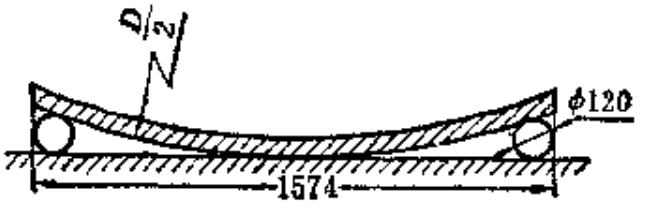
\includegraphics[width=7cm]{../pic/czjh2-ch7-fuxi-21.png}
    \caption*{(第 21 题)}
\end{figure}

\xiaoti{半径为 $R$ 和 $r$ ($R > r$) 的两圆相外切。求一条外公切线的长。}

\xiaoti{画出图中由圆和弧所组成的图案。}

\begin{figure}[htbp]
    \centering
    \begin{minipage}[b]{4cm}
        \centering
        \begin{tikzpicture}
    \pgfmathsetmacro{\R}{1.5}
    \pgfmathsetmacro{\r}{\R/2}

    \tkzDefPoints{0/0/O}
    \tkzDefPoint(180:\R){A}
    \tkzDefPoint(0:\R){B}
    \tkzDefPoint(180:\r){O_1}
    \tkzDefPoint(0:\r){O_2}

    \tkzDrawCircle[thick](O,A)
    \tkzDrawArc(O_1,O)(A)
    \tkzDrawArc(O_2,O)(B)
    \tkzDrawSegment[dashed](A,B)
\end{tikzpicture}


        \caption*{甲}
    \end{minipage}
    \begin{minipage}[b]{4cm}
        \centering
        \begin{tikzpicture} % 复杂
    \pgfmathsetmacro{\R}{1}

    \tkzDefPoints{0/0/O}
    \tkzDefPoint(0:\R){A}
    \tkzDefRegPolygon[center,sides=4,name=P](O,A)
    \tkzCalcLength(P1,P2)  \tkzGetLength{PP}
    \tkzInterCC[R](P1,\PP)(P2,\PP)  \tkzGetSecondPoint{B}
    \tkzDefRegPolygon[center,sides=4,name=Q](O,B)
    % \tkzLabelPoints[centered](P1,P...,P4)
    % \tkzLabelPoints[centered](Q1,Q...,Q4)

    \tkzDrawCircle[thick](O,A)
    \tkzDrawSegments[dashed](P1,P3  P2,P4)

    \foreach \i in {1,...,4} {
        \ifnum\i=4\relax
            \pgfmathsetmacro{\n}{1}
        \else
            \pgfmathsetmacro{\n}{int(\i+1)}
        \fi

        \tkzDrawArc[R with nodes](P\n,\PP)(P\i,Q\i)
        \tkzDrawArc[R with nodes](P\i,\PP)(Q\i,P\n)
    }
\end{tikzpicture}


        \caption*{乙}
    \end{minipage}
    \begin{minipage}[b]{4cm}
        \centering
        \begin{tikzpicture} % 复杂
    \pgfmathsetmacro{\R}{1.2}
    \pgfmathsetmacro{\RR}{sqrt(2)*\R}
    \pgfmathsetmacro{\r}{\RR/2}

    \tkzDefPoints{0/0/O}
    \tkzDefPoint(0:\R){A}
    \tkzDefRegPolygon[center,sides=4,name=P](O,A)
    \tkzDefPoint(45:\RR){B}
    \tkzDefRegPolygon[center,sides=4,name=Q](O,B)
    \tkzDefPoint(45:\r){C}
    \tkzDefRegPolygon[center,sides=4,name=O](O,C)
    % \tkzLabelPoints[centered](P1,P...,P4)
    % \tkzLabelPoints[centered](Q1,Q...,Q4)
    % \tkzLabelPoints[centered](O1,O...,O4)

    \tkzDrawSegments[dashed](P1,P3  P2,P4)
    \tkzDrawPolygon[dashed](Q1,Q...,Q4)

    \foreach \i in {1,...,4} {
        \ifnum\i=4\relax
            \pgfmathsetmacro{\n}{1}
        \else
            \pgfmathsetmacro{\n}{int(\i+1)}
        \fi

        \tkzDrawArc[R with nodes](O\i,\r)(P\i,P\n)
    }
\end{tikzpicture}


        \caption*{丙}
    \end{minipage}
    \begin{minipage}[b]{4cm}
        \centering
        \begin{tikzpicture} % 复杂
    \pgfmathsetmacro{\R}{1.5}
    \pgfmathsetmacro{\RR}{sqrt(2)*\R}
    \pgfmathsetmacro{\r}{\RR/2}

    \tkzDefPoints{0/0/O}
    \tkzDefPoint(0:\R){A}
    \tkzDefRegPolygon[center,sides=4,name=P](O,A)
    \tkzDefPoint(45:\RR){B}
    \tkzDefRegPolygon[center,sides=4,name=Q](O,B)
    \tkzDefPoint(45:\r){C}
    \tkzDefRegPolygon[center,sides=4,name=O](O,C)
    % \tkzLabelPoints[centered](P1,P...,P4)
    % \tkzLabelPoints[centered](Q1,Q...,Q4)
    % \tkzLabelPoints[centered](O1,O...,O4)
    % \tkzLabelPoints[centered](O)

    \tkzDrawPolygon[dashed](Q1,Q...,Q4)
    % \tkzDrawPolygon[dashed](P1,P...,P4)
    % \tkzDrawPolygon[dashed](O1,O...,O4)

    \foreach \i in {1,...,4} {
        \ifnum\i=4\relax
            \pgfmathsetmacro{\n}{1}
        \else
            \pgfmathsetmacro{\n}{int(\i+1)}
        \fi

        \tkzDrawArc[](P\n,Q\n)(Q\i)
    }

    \foreach \i in {1,...,4} {
        \ifnum\i=4\relax
            \pgfmathsetmacro{\n}{1}
        \else
            \pgfmathsetmacro{\n}{int(\i+1)}
        \fi

        \begin{scope}
            \tkzClipPolygon[out](O,P\i,Q\i,P\n)
            \tkzDrawArc[fill=white](O\i,P\n)(P\i)
        \end{scope}
    }
\end{tikzpicture}


        \caption*{丁}
    \end{minipage}
    \caption*{(第 23 题)}
\end{figure}


\xiaoti{正十边形的边长为 $2a$, 求它的面积(用代数式表示)。}

\xiaoti{我国民间相传有正五边形的近似作法。“九五顶五九,八五分两边”,它的意义如图所示。}
\begin{xiaoxiaotis}

    \xxt{用这个方法作边长为 50 毫米的近似正五边形;}

    \xxt{用三角函数计算边长为 10 寸的正五边形中,相当于图中 5.9 寸、9.5 寸、8 寸的线段的长,加以比较。}

\end{xiaoxiaotis}

\begin{figure}[htbp]
    \centering
    \begin{minipage}[b]{7cm}
        \centering
        \begin{tikzpicture}
    \pgfmathsetmacro{\factor}{0.25}

    \tkzDefPoint(0,0){O}
    \tkzDefPoint(5*\factor,0){A}
    \tkzDefPoint(8*\factor,9.5*\factor){B}
    \tkzDefPoint(0,(9.5+5.9)*\factor){C}
    \tkzDefPoint(-8*\factor,9.5*\factor){D}
    \tkzDefPoint(-5*\factor,0){E}
    \tkzDefPoint(0,9.5*\factor){F}
    % \tkzLabelPoints[centered](A,...,F,O)

    \tkzDrawPolygon(A,...,E)
    \tkzDrawSegments(B,D  O,C)
    \tkzLabelSegment[above, sloped](O,F){9.5寸}
    \tkzLabelSegment[pos=.4, above, sloped](F,C){5.9寸}
    \tkzLabelSegment[below](F,B){8寸}
    \tkzLabelSegment[below](F,D){8寸}
    \tkzLabelSegment[below](O,A){5寸}
    \tkzLabelSegment[below](O,E){5寸}
\end{tikzpicture}


        \caption*{(第 25 题)}
    \end{minipage}
    \qquad
    \begin{minipage}[b]{7cm}
        \centering
        \begin{tikzpicture}
    \pgfmathsetmacro{\R}{3}
    \pgfmathsetmacro{\r}{2}

    \tkzDefPoint(0,0){O}
    \tkzDefPoint(130:\R){A}
    \tkzDefPoint(130:\r){A'}
    \tkzDefPoint(60:\R){B}
    \tkzDefPoint(60:\r){B'}

    \tkzFillSector[pattern={mylines[angle=45, distance={3pt}]}](O,B)(A)
    \tkzFillSector[fill=white](O,B')(A')
    \tkzDrawSector[thick](O,B)(A)
    \tkzDrawArc[thick](O,B')(A')
    \tkzLabelArc[above](O,B,A){$l$}
    \tkzLabelArc[below](O,B',A'){$l'$}
    \tkzLabelSegment[centered, rotate=40, xshift=-.6em](A,A'){$d$}
    \tkzLabelPoints[below](O)
    \tkzLabelPoints[below left](A,A')
    \tkzLabelPoints[right](B,B')
\end{tikzpicture}


        \caption*{(第 29 题)}
    \end{minipage}
\end{figure}

\xiaoti{求证:两个同心圆所成环形的面积等于以切于小圆的大圆的弦为直径的圆的面积。}

\xiaoti{半径为 $R$ 的两个等圆互相经过圆心,求两圆所围的公共部分的面积。}

\xiaoti{已知:直角三角形 $ABC$ 及斜边 $BC$ 上的高 $AD$。
    求证: $\triangle ABD$ 和 $\triangle ACD$ 的内切圆的面积的比等于 $BD:DC$。
}

\xiaoti{如图, $\yuanhu{AB}$ 与 $\yuanhu{A'B'}$ 的圆心都是 $O$,
    $AA' = d$, $\yuanhu{AB}$ 的长是 $l$, $\yuanhu{A'B'}$ 的长是 $l'$。求证:
}
\begin{xiaoxiaotis}

    \xxt{$\angle O = \dfrac{l - l'}{d} \times \dfrac{180}{\pi}$ 度;}

    \xxt{$S_{AA'B'B} = \exdfrac{1}{2} (l + l') \, d$。}
\end{xiaoxiaotis}

\xiaoti{如图, $B$ 是 $AC$ 上的一点, 分别以 $AB$、$BC$、$AC$ 为直径作半圆。
    从 $B$ 作 $BD \perp AC$, 与半圆相交于 $D$。
    求证:图中阴影部分的面积等于以BD为直径的圆的面积。
}

\begin{figure}[htbp]
    \centering
    \begin{minipage}[b]{7cm}
        \centering
        \begin{tikzpicture}
    \tkzDefPoints{0/0/A, 4/0/C}
    \tkzDefPointOnLine[pos=0.4](A,C)  \tkzGetPoint{B}
    \tkzDefMidPoint(A,C)  \tkzGetPoint{O}
    \tkzDefMidPoint(A,B)  \tkzGetPoint{O1}
    \tkzDefMidPoint(B,C)  \tkzGetPoint{O2}
    \tkzDefLine[perpendicular=through B](A,C)  \tkzGetPoint{d}
    \tkzInterLC(B,d)(O,A)  \tkzGetFirstPoint{D}
    \tkzDefMidPoint(B,D)  \tkzGetPoint{O3}

    \tkzFillSector[pattern={mylines[angle=45, distance={3pt}]}](O,C)(A)
    \tkzFillSector[fill=white](O1,B)(A)
    \tkzFillSector[fill=white](O2,C)(B)
    \tkzDrawArc[thick](O,C)(A)
    \tkzDrawArc[thick](O1,B)(A)
    \tkzDrawArc[thick](O2,C)(B)
    \tkzDrawCircle[very thick](O3,B)
    \tkzDrawSegments[thick](A,C  B,D)
    \tkzLabelPoints[below](A,B,C)
    \tkzLabelPoints[above](D)
\end{tikzpicture}


        \caption*{(第 30 题)}
    \end{minipage}
    \qquad
    \begin{minipage}[b]{7cm}
        \centering
        \begin{tikzpicture}
    \pgfmathsetmacro{\factor}{0.1}

    % 坐标
    \tkzDefPoints{-15*\factor/0/x1, 50*\factor/0/x2, 0/-15*\factor/y1, 0/22*\factor/y2}
    \tkzDrawSegments[-|Latex](x1,x2  y1,y2)
    \tkzLabelSegment[pos=1, below](x1,x2){$x$}
    \tkzLabelSegment[pos=1, left](y1,y2){$y$}

    % 圆 O
    \pgfmathsetmacro{\Ra}{10*\factor}
    \tkzDefPoint(0,0){O}
    \tkzDefPoint(100:\Ra){L}
    \tkzDrawCircle[thick](O,L)
    \tkzDrawSegment[-Latex](O,L)
    \tkzLabelSegment[pos=.3, left](O,L){$R10$}
    \tkzLabelPoints[below left](O)

    % 圆 O_1
    \pgfmathsetmacro{\Rb}{8*\factor}
    \tkzDefPoint(35*\factor,0){O_1}
    \tkzDefShiftPoint[O_1](100:\Rb){M}
    \tkzDrawCircle[thick](O_1,M)
    \tkzDrawSegment[-Latex](O_1,M)
    \tkzLabelSegment[right=-.2em](O_1,M){$R8$}
    \tkzLabelPoints[below](O_1)


    % 点 P 及弧线
    \pgfmathsetmacro{\Rc}{27*\factor}
    \tkzDefPoint(31.90*\factor,18.75*\factor){P}
    \tkzDefShiftPoint[P](240:\Rc){N}
    \tkzInterLC[R](O,P)(O,\Ra)  \tkzGetSecondPoint{A}
    \tkzInterLC[R](O_1,P)(O_1,\Rb)  \tkzGetSecondPoint{B}
    \tkzDrawArc[dashed](P,A)(B)
    \tkzDrawSegment[-Latex](P,N)
    \tkzLabelSegment[above, sloped](P,N){$R27$}
    \tkzDrawPoint(P)
    \tkzLabelPoints[right](A)
    \tkzLabelPoints[below](B)
    \tkzLabelPoint[right](P){$P(x,y)$}
\end{tikzpicture}


        \caption*{(第 35 题)}
    \end{minipage}
\end{figure}

\xiaoti{}%
\begin{xiaoxiaotis}%
    \xxt[\xxtsep]{举出原命题和逆命题都正确以及原命题正确而逆命题不正确的例子;}

    \xxt{举出原命题和否命题都正确以及原命题正确而否命题不正确的例子;}

    \xxt{能不能举出原命题正确而逆否命题不正确的例子?为什么?}

\end{xiaoxiaotis}

\xiaoti{图形 $F$ 是符合条件 $C$ 的点的轨迹,需要下列两个命题都正确:
    1. 图形 $F$ 上的每一个点都符合条件 $C$;
    2. 符合条件 $C$ 的每一个点都在图形 $F$ 上。
}
\begin{xiaoxiaotis}

    \xxt{如果命题 1 正确,命题 2 不正确,会发生什么情况?举例说明;}

    \xxt{如果命题 1 不正确,命题 2 正确,会发生什么情况?举例说明。}
\end{xiaoxiaotis}

\xiaoti{已知 $\yuan\,O$ 上一点 $A$,说明并作出以点 $A$ 为端点的弦的中点的轨迹(不要求证明)。}

\xiaoti{求作一个圆,使它的半径等于 3 cm, 经过已知点 $A$,并且和半径为 2 cm 的已知圆 $O$ 相切(已知 $OA = 6$ cm)。}

\xiaoti{在如图所示的坐标系中, $\yuan\,O$ 的半径为 10, $O_1 $的坐标为 $(35, 0)$,
    $\yuan\,O_1$ 的半径为 8。 $\yuanhu{AB}$ 与 $\yuan\,O$ 上的弧外连接,
    与 $\yuan\,O_1$ 上的弧内连接。计算 $\yuanhu{AB}$ 所在圆的圆心 $P$ 的坐标(保留4个有效数字)。
}


\end{enhancedline}
\end{xiaotis}



\nonumsection{附录 圆周长和圆面积}\mylabel{sec:czjh2-7-fulu}
\begin{enhancedline}

我们早就学过:“$\text{圆周长} = \text{直径} \times \text{圆周率}\;\pi$”。
可是,圆周长与直径的比值,即圆周率 $\pi$ 的值是怎样计算出来的呢?

在半径为 $R$ 的圆中(图 \ref{fig:czjh2-7-86}),内接正六边形的周长是 $p_6 = 6R$,
圆内接正六边形的周长与圆的直径的比是 $\dfrac{6R}{2R} = 3$,
这个比值与 $R$ 无关,也就是说,不管圆的大小怎样,它是一个常数。

\begin{figure}[htbp]
    \centering
    \begin{minipage}[b]{7cm}
        \centering
        \begin{tikzpicture}
    \pgfmathsetmacro{\R}{1.5}
    \tkzDefPoints{0/0/O}
    \tkzDefPoint(60:\R){A}
    \tkzDrawCircle[very thick](O,A)
    \tkzDrawSegment(O,A)
    \tkzDrawPoint(O)
    \tkzLabelSegment[right](O,A){$R$}
    \tkzLabelPoints[left](O)

    \tkzDefRegPolygon[center,sides=6,name=P](O,A)
    \tkzDrawPolygon[thick,red](P1,P...,P6)

    \tkzDefRegPolygon[center,sides=12,name=P](O,A)
    \tkzDrawPolygon[thick,blue](P1,P...,P12)
\end{tikzpicture}


        \caption{}\label{fig:czjh2-7-86}
    \end{minipage}
    \qquad
    \begin{minipage}[b]{7cm}
        \centering
        \begin{tikzpicture}
    \pgfmathsetmacro{\R}{1.5}
    \tkzDefPoints{0/0/O}
    \tkzDefPoint(230:\R){A}
    \tkzDefPoint(310:\R){B}
    \tkzDefLine[altitude](A,O,B)  \tkzGetPoint{D}
    \tkzInterLC(O,D)(O,A)  \tkzGetSecondPoint{C}

    \tkzDrawCircle[very thick](O,A)
    \tkzDrawSegments(A,B  O,C  A,C)
    \tkzDrawSegments[dashed](O,A  O,B)
    \tkzDrawPoint(O)
    \tkzMarkRightAngle[size=.2](B,D,O)
    \tkzLabelSegment[above, xshift=-.2em](O,A){$R$}
    \tkzLabelPoints[above](O)
    \tkzLabelPoints[left=.2em](A)
    \tkzLabelPoints[right=.2em](B)
    \tkzLabelPoints[below](C)
    \tkzLabelPoints[above, xshift=.5em, yshift=.3em](D)
\end{tikzpicture}


        \caption{}\label{fig:czjh2-7-87}
    \end{minipage}
\end{figure}

如果把圆内接正 6 边形的周长看作是圆的周长的近似值,
把圆内接正 6 边形的周长与直径的比(等于3) 看作是圆的周长与直径的比的近似值,
当然,误差是很大的。

把圆内接正 6 边形的边数加倍,可以得到圆内接正 12 边形;
再加倍,可以得到圆内接正 24 边形; ……。
我们可以把这样一些圆内接正多边形的周长看作是圆的周长的近似值,
把这些圆内接正多边形的周长与直径的比作为圆的周长与直径的比的近似值。
当圆内接正多边形的边数不断地成倍增加时,它们的周长 $p_n$ 不断地增大,越来越接近于圆的周长, % 书中原文为 P_n,但结合上下文,写为 p_n 更合适。下一行也是这样。
圆内接正多边形的周长 $p_n$ 和直径 $2R$ 的比值就越来越接近于圆周长 $C$ 和直径 $2R$ 的比值,
误差越来越小,只要边数 $n$ 充分大,误差可以任意地小。

为了说明,我们先证明下列 “倍边公式”。

设 $\yuan\,O$ 的半径为 $R$ (图 \ref{fig:czjh2-7-87}),
圆内接正 $n$ 边形及正 $2n$ 边形的边长分别为 $AB = a_n$ 及 $AC = a_{2n}$。
因为半径 $OC$ 垂直平分 $AB$,由勾股定理可知,

$\begin{aligned}
    a_{2n}^2 &= AC^2 = AD^2 + CD^2 \\
             &= AD^2 + (OC - OD)^2 \\
             &= AD^2 + (OC - \sqrt{OA^2 - AD^2})^2 \\
             &= AD^2 + OC^2 - 2 OC \sqrt{OA^2 - AD^2} + OA^2 - AD^2 \\
             &= OC^2 + OA^2 - 2 OC \sqrt{OA^2 - AD^2} \\
             &= 2R^2 - 2R \sqrt{R^2 - \exdfrac{1}{4} a_n^2} \juhao
\end{aligned}$

$\therefore$ \quad $a_{2n} = \sqrt{2R^2 - R \sqrt{4R^2 - a_n^2}}$。

由于 $a_6 = R$,依据这个公式,就可依次计算得
\begin{align*}
    & a_{12} = \sqrt{2 - \sqrt{3\,}} \, R \fenhao \\
    & a_{24} = \sqrt{2 - \sqrt{2 + \sqrt{3\,}}} \, R \fenhao \\
    & a_{48} = \sqrt{2 - \sqrt{2 + \sqrt{2 + \sqrt{3\,}}}} \, R \fenhao \\
    & \cdots \cdots
\end{align*}
利用这个等式,半径为 $R$ 的圆内接正 6、12、24、… 边形的边长、周长以及周长与直径的比,
就都可以计算出来(如下表)。% 如下页表

可以看出,每一个圆内接正 $n$ 边形的周长和直径的比 $\left(\dfrac{p_n}{2R}\right)$
都是与半径 $R$ 无关的常数,所以,圆的周长和直径的比 $\left(\dfrac{C}{2R}\right)$
也是一个与 $R$ 无关的常数,这个常数就是 $\pi$。


\begin{tblr}{hlines, vlines,
    columns={c},
}
    边数$n$ & 边长 $a_n$ & 周长 $p_n$ & 周长与直径的比 $\dfrac{p_n}{2R}$ \\
    6   & 1.00000000 $R$ & 6.00000000 $R$ & 3.00000000 \\
    12  & 0.51763809 $R$ & 6.21165708 $R$ & 3.10582854 \\
    24  & 0.26105238 $R$ & 6.26525722 $R$ & 3.13262861 \\
    48  & 0.13080626 $R$ & 6.27870041 $R$ & 3.13935021 \\
    96  & 0.06543817 $R$ & 6.28206396 $R$ & 3.14103198 \\
    192 & 0.03272316 $R$ & 6.28290510 $R$ & 3.14145255 \\
    384 & 0.01636228 $R$ & 6.28311544 $R$ & 3.14155772 \\
    768 & 0.00818121 $R$ & 6.28316941 $R$ & 3.14158471 \\
\end{tblr}


这样,我们就得到了一种计算圆周率 $\pi$ 的近似值的方法。

我国古代数学家祖冲之,在公元五世纪就已算得 $\pi$ 的值在 3.1415926 与 3.1415927 之间,
比其他国家早一千年左右。现代利用电子计算机,已有人把 $\pi$ 的值算到小数点后几十万位。
$\pi$ 是一个无限不循环小数,就是说,是一个无理数。

\begin{wrapfigure}[10]{r}{6cm}
    \centering
    \begin{tikzpicture}
    \pgfmathsetmacro{\R}{2}
    \tkzDefPoints{0/0/O}
    \tkzDefPoint(60:\R){A}
    \tkzDrawCircle[very thick](O,A)
    \tkzDrawSegment(O,A)
    \tkzLabelSegment[left](O,A){$R$}
    \tkzLabelPoints[left](O)

    \tkzDefRegPolygon[center,sides=6,name=P](O,A)
    \tkzDrawPolygon[thick,red](P1,P...,P6)
    \tkzDefMidPoint(P4,P5)  \tkzGetPoint{H}
    \tkzDrawSegment(O,H)
    \tkzLabelSegment[right](O,H){$r_n$}

    \tkzDefRegPolygon[center,sides=12,name=P](O,A)
    \tkzDrawPolygon[thick,blue](P1,P...,P12)
\end{tikzpicture}


    \caption{}\label{fig:czjh2-7-88}
\end{wrapfigure}

由于 $\dfrac{C}{2R} = \pi$, 就可得到圆周长的计算公式
$$ C = 2 \pi R \juhao $$

此外,我们知道,如图 \ref{fig:czjh2-7-88}, 边心距为 $r_n$、周长为 $p_n$ 的正 $n$ 边形的面积 $S_n$ 等于 $\exdfrac{1}{2} r_n p_n$ 。

在半径为 $R$ 的圆中,当内接正多边形的边数不断地成倍增加时,
正多边形的边心距 $r_n$ 越来越接近于圆的半径 $R$,
正多边形的周长 $p_n$ 越来越接近于圆周长 $C$,
而正多边形的面积 $S_n$ 就越来越接近于圆面积 $S$。
这样,从正 $n$ 边形的面积公式 $S_n = \exdfrac{1}{2} r_n p_n$ 就可以得到圆面积公式
$$ S = \exdfrac{1}{2} R \cdot C = \exdfrac{1}{2} R \cdot 2 \pi R = \pi R^2 \juhao $$

\end{enhancedline}




